\documentclass[12pt]{book}
\usepackage[utf8]{inputenc}
\usepackage[english, spanish]{babel}
\renewcommand\spanishtablename{Tabla}
\usepackage{booktabs}
\usepackage{todonotes}
\usepackage{tikz}
\usepackage{paralist}
\usepackage{subcaption}
\usepackage{graphicx}
\usepackage{amsmath} \usepackage{amssymb}
\usepackage{xcolor}
\usepackage{caption}
%\captionsetup{font=scriptsize}
\captionsetup[subfigure]{font=small}
\DeclareCaptionFormat{figformat}{#1#2#3\hrulefill}
\captionsetup[figure]{format=figformat}
\captionsetup[subfigure]{format=default}

\newcommand{\mysquare}[2]{\tikz{\filldraw[draw=#1,fill=#2] (0,0)
rectangle (0.2cm,0.2cm);}}

\newcommand{\mycircle}[2]{\tikz{\filldraw[draw=#1,fill=#2] (0,0) circle [radius=0.1cm];}}

\newcommand{\mytriangle}[2]{\tikz{\filldraw[draw=#1,fill=#2] (0,0) --
(0.2cm,0) -- (0.1cm,0.2cm) -- (0, 0);}}

\newcommand{\mydiamond}[2]{\tikz{\filldraw[draw=#1,fill=#2] (0.1cm,0cm) --
(0.2cm,0.1cm) -- (0.1cm,0.2cm) -- (0cm,0.1cm) -- (0.1cm,0cm);}}

\definecolor{color1}{RGB}{102,194,165}
\definecolor{color2}{RGB}{252,141,98}
\definecolor{color3}{RGB}{141,160,203}
\definecolor{color4}{RGB}{231,138,195}

%\usepackage{geometry}
\usepackage{hyperref}
%\usepackage{kpfonts}
\usepackage{subcaption}
\linespread{1.3}
\usepackage{natbib}
\bibliographystyle{alpha}
%%%%%%%%%%%%%%%%%%%%%%%%%%%%%%%%%%%%%%%%%
% The Legrand Orange Book
% Structural Definitions File
% Version 2.0 (9/2/15)
%
% Original author:
% Mathias Legrand (legrand.mathias@gmail.com) with modifications by:
% Vel (vel@latextemplates.com)
% 
% This file has been downloaded from:
% http://www.LaTeXTemplates.com
%
% License:
% CC BY-NC-SA 3.0 (http://creativecommons.org/licenses/by-nc-sa/3.0/)
%
%%%%%%%%%%%%%%%%%%%%%%%%%%%%%%%%%%%%%%%%%

%----------------------------------------------------------------------------------------
%	VARIOUS REQUIRED PACKAGES AND CONFIGURATIONS
%----------------------------------------------------------------------------------------

\usepackage[top=3cm,bottom=3cm,left=3cm,right=3cm,headsep=10pt,a4paper]{geometry} % Page margins

\usepackage{graphicx} % Required for including pictures
\graphicspath{{Pictures/}} % Specifies the directory where pictures are stored

\usepackage{lipsum} % Inserts dummy text

\usepackage{tikz} % Required for drawing custom shapes

\usepackage[english]{babel} % English language/hyphenation

\usepackage{enumitem} % Customize lists
\setlist{nolistsep} % Reduce spacing between bullet points and numbered lists

\usepackage{booktabs} % Required for nicer horizontal rules in tables

\usepackage{xcolor} % Required for specifying colors by name
\definecolor{ocre}{RGB}{243,102,25} % Define the orange color used for highlighting throughout the book

%----------------------------------------------------------------------------------------
%	FONTS
%----------------------------------------------------------------------------------------

\usepackage{avant} % Use the Avantgarde font for headings
\usepackage{times} % Use the Times font for headings
\usepackage{mathptmx} % Use the Adobe Times Roman as the default text font together with math symbols from the Sym­bol, Chancery and Com­puter Modern fonts

\usepackage{microtype} % Slightly tweak font spacing for aesthetics
\usepackage[utf8]{inputenc} % Required for including letters with accents
\usepackage[T1]{fontenc} % Use 8-bit encoding that has 256 glyphs

%----------------------------------------------------------------------------------------
%	BIBLIOGRAPHY AND INDEX
%----------------------------------------------------------------------------------------

%\usepackage[style=numeric,citestyle=numeric,sorting=nyt,sortcites=true,autopunct=true,babel=hyphen,hyperref=true,abbreviate=false,backref=true,backend=biber]{biblatex}
%\addbibresource{bibliography.bib} % BibTeX bibliography file
%\defbibheading{bibempty}{}

\usepackage{calc} % For simpler calculation - used for spacing the index letter headings correctly
\usepackage{makeidx} % Required to make an index
\makeindex % Tells LaTeX to create the files required for indexing

%----------------------------------------------------------------------------------------
%	MAIN TABLE OF CONTENTS
%----------------------------------------------------------------------------------------

\usepackage{titletoc} % Required for manipulating the table of contents

\contentsmargin{0cm} % Removes the default margin

% Part text styling
\titlecontents{part}[0cm]
{\addvspace{20pt}\centering\large\bfseries}
{}
{}
{}

% Chapter text styling
\titlecontents{chapter}[1.25cm] % Indentation
{\addvspace{12pt}\large\sffamily\bfseries} % Spacing and font options for chapters
{\color{ocre!60}\contentslabel[\Large\thecontentslabel]{1.25cm}\color{ocre}} % Chapter number
{\color{ocre}}  
{\color{ocre!60}\normalsize\;\titlerule*[.5pc]{.}\;\thecontentspage} % Page number

% Section text styling
\titlecontents{section}[1.25cm] % Indentation
{\addvspace{3pt}\sffamily\bfseries} % Spacing and font options for sections
{\contentslabel[\thecontentslabel]{1.25cm}} % Section number
{}
{\hfill\color{black}\thecontentspage} % Page number
[]

% Subsection text styling
\titlecontents{subsection}[1.25cm] % Indentation
{\addvspace{1pt}\sffamily\small} % Spacing and font options for subsections
{\contentslabel[\thecontentslabel]{1.25cm}} % Subsection number
{}
{\ \titlerule*[.5pc]{.}\;\thecontentspage} % Page number
[]

% List of figures
\titlecontents{figure}[0em]
{\addvspace{-5pt}\sffamily}
{\thecontentslabel\hspace*{1em}}
{}
{\ \titlerule*[.5pc]{.}\;\thecontentspage}
[]

% List of tables
\titlecontents{table}[0em]
{\addvspace{-5pt}\sffamily}
{\thecontentslabel\hspace*{1em}}
{}
{\ \titlerule*[.5pc]{.}\;\thecontentspage}
[]

%----------------------------------------------------------------------------------------
%	MINI TABLE OF CONTENTS IN PART HEADS
%----------------------------------------------------------------------------------------

% Chapter text styling
\titlecontents{lchapter}[0em] % Indenting
{\addvspace{15pt}\large\sffamily\bfseries} % Spacing and font options for chapters
{\color{ocre}\contentslabel[\Large\thecontentslabel]{1.25cm}\color{ocre}} % Chapter number
{}  
{\color{ocre}\normalsize\sffamily\bfseries\;\titlerule*[.5pc]{.}\;\thecontentspage} % Page number

% Section text styling
\titlecontents{lsection}[0em] % Indenting
{\sffamily\small} % Spacing and font options for sections
{\contentslabel[\thecontentslabel]{1.25cm}} % Section number
{}
{}

% Subsection text styling
\titlecontents{lsubsection}[.5em] % Indentation
{\normalfont\footnotesize\sffamily} % Font settings
{}
{}
{}

%----------------------------------------------------------------------------------------
%	PAGE HEADERS
%----------------------------------------------------------------------------------------

\usepackage{fancyhdr} % Required for header and footer configuration

\pagestyle{fancy}
\renewcommand{\chaptermark}[1]{\markboth{\sffamily\normalsize\bfseries\chaptername\ \thechapter.\ #1}{}} % Chapter text font settings
\renewcommand{\sectionmark}[1]{\markright{\sffamily\normalsize\thesection\hspace{5pt}#1}{}} % Section text font settings
\fancyhf{} \fancyhead[LE,RO]{\sffamily\normalsize\thepage} % Font setting for the page number in the header
\fancyhead[LO]{\rightmark} % Print the nearest section name on the left side of odd pages
\fancyhead[RE]{\leftmark} % Print the current chapter name on the right side of even pages
\renewcommand{\headrulewidth}{0.5pt} % Width of the rule under the header
\addtolength{\headheight}{2.5pt} % Increase the spacing around the header slightly
\renewcommand{\footrulewidth}{0pt} % Removes the rule in the footer
\fancypagestyle{plain}{\fancyhead{}\renewcommand{\headrulewidth}{0pt}} % Style for when a plain pagestyle is specified

% Removes the header from odd empty pages at the end of chapters
\makeatletter
\renewcommand{\cleardoublepage}{
\clearpage\ifodd\c@page\else
\hbox{}
\vspace*{\fill}
\thispagestyle{empty}
\newpage
\fi}

%----------------------------------------------------------------------------------------
%	THEOREM STYLES
%----------------------------------------------------------------------------------------

\usepackage{amsmath,amsfonts,amssymb,amsthm} % For math equations, theorems, symbols, etc

\newcommand{\intoo}[2]{\mathopen{]}#1\,;#2\mathclose{[}}
\newcommand{\ud}{\mathop{\mathrm{{}d}}\mathopen{}}
\newcommand{\intff}[2]{\mathopen{[}#1\,;#2\mathclose{]}}
\newtheorem{notation}{Notation}[chapter]

% Boxed/framed environments
\newtheoremstyle{ocrenumbox}% % Theorem style name
{0pt}% Space above
{0pt}% Space below
{\normalfont}% % Body font
{}% Indent amount
{\small\bf\sffamily\color{ocre}}% % Theorem head font
{\;}% Punctuation after theorem head
{0.25em}% Space after theorem head
{\small\sffamily\color{ocre}\thmname{#1}\nobreakspace\thmnumber{\@ifnotempty{#1}{}\@upn{#2}}% Theorem text (e.g. Theorem 2.1)
\thmnote{\nobreakspace\the\thm@notefont\sffamily\bfseries\color{black}---\nobreakspace#3.}} % Optional theorem note
\renewcommand{\qedsymbol}{$\blacksquare$}% Optional qed square

\newtheoremstyle{blacknumex}% Theorem style name
{5pt}% Space above
{5pt}% Space below
{\normalfont}% Body font
{} % Indent amount
{\small\bf\sffamily}% Theorem head font
{\;}% Punctuation after theorem head
{0.25em}% Space after theorem head
{\small\sffamily{\tiny\ensuremath{\blacksquare}}\nobreakspace\thmname{#1}\nobreakspace\thmnumber{\@ifnotempty{#1}{}\@upn{#2}}% Theorem text (e.g. Theorem 2.1)
\thmnote{\nobreakspace\the\thm@notefont\sffamily\bfseries---\nobreakspace#3.}}% Optional theorem note

\newtheoremstyle{blacknumbox} % Theorem style name
{0pt}% Space above
{0pt}% Space below
{\normalfont}% Body font
{}% Indent amount
{\small\bf\sffamily}% Theorem head font
{\;}% Punctuation after theorem head
{0.25em}% Space after theorem head
{\small\sffamily\thmname{#1}\nobreakspace\thmnumber{\@ifnotempty{#1}{}\@upn{#2}}% Theorem text (e.g. Theorem 2.1)
\thmnote{\nobreakspace\the\thm@notefont\sffamily\bfseries---\nobreakspace#3.}}% Optional theorem note

% Non-boxed/non-framed environments
\newtheoremstyle{ocrenum}% % Theorem style name
{5pt}% Space above
{5pt}% Space below
{\normalfont}% % Body font
{}% Indent amount
{\small\bf\sffamily\color{ocre}}% % Theorem head font
{\;}% Punctuation after theorem head
{0.25em}% Space after theorem head
{\small\sffamily\color{ocre}\thmname{#1}\nobreakspace\thmnumber{\@ifnotempty{#1}{}\@upn{#2}}% Theorem text (e.g. Theorem 2.1)
\thmnote{\nobreakspace\the\thm@notefont\sffamily\bfseries\color{black}---\nobreakspace#3.}} % Optional theorem note
\renewcommand{\qedsymbol}{$\blacksquare$}% Optional qed square
\makeatother

% Defines the theorem text style for each type of theorem to one of the three styles above
\newcounter{dummy} 
\numberwithin{dummy}{section}
\theoremstyle{ocrenumbox}
\newtheorem{theoremeT}[dummy]{Theorem}
\newtheorem{problem}{Problem}[chapter]
\newtheorem{exerciseT}{Exercise}[chapter]
\theoremstyle{blacknumex}
\newtheorem{exampleT}{Example}[chapter]
\theoremstyle{blacknumbox}
\newtheorem{vocabulary}{Vocabulary}[chapter]
\newtheorem{definitionT}{Definition}[section]
\newtheorem{corollaryT}[dummy]{Corollary}
\theoremstyle{ocrenum}
\newtheorem{proposition}[dummy]{Proposition}

%----------------------------------------------------------------------------------------
%	DEFINITION OF COLORED BOXES
%----------------------------------------------------------------------------------------

\RequirePackage[framemethod=default]{mdframed} % Required for creating the theorem, definition, exercise and corollary boxes

% Theorem box
\newmdenv[skipabove=7pt,
skipbelow=7pt,
backgroundcolor=black!5,
linecolor=ocre,
innerleftmargin=5pt,
innerrightmargin=5pt,
innertopmargin=5pt,
leftmargin=0cm,
rightmargin=0cm,
innerbottommargin=5pt]{tBox}

% Exercise box	  
\newmdenv[skipabove=7pt,
skipbelow=7pt,
rightline=false,
leftline=true,
topline=false,
bottomline=false,
backgroundcolor=ocre!10,
linecolor=ocre,
innerleftmargin=5pt,
innerrightmargin=5pt,
innertopmargin=5pt,
innerbottommargin=5pt,
leftmargin=0cm,
rightmargin=0cm,
linewidth=4pt]{eBox}	

% Definition box
\newmdenv[skipabove=7pt,
skipbelow=7pt,
rightline=false,
leftline=true,
topline=false,
bottomline=false,
linecolor=ocre,
innerleftmargin=5pt,
innerrightmargin=5pt,
innertopmargin=0pt,
leftmargin=0cm,
rightmargin=0cm,
linewidth=4pt,
innerbottommargin=0pt]{dBox}	

% Corollary box
\newmdenv[skipabove=7pt,
skipbelow=7pt,
rightline=false,
leftline=true,
topline=false,
bottomline=false,
linecolor=gray,
backgroundcolor=black!5,
innerleftmargin=5pt,
innerrightmargin=5pt,
innertopmargin=5pt,
leftmargin=0cm,
rightmargin=0cm,
linewidth=4pt,
innerbottommargin=5pt]{cBox}

% Creates an environment for each type of theorem and assigns it a theorem text style from the "Theorem Styles" section above and a colored box from above
\newenvironment{theorem}{\begin{tBox}\begin{theoremeT}}{\end{theoremeT}\end{tBox}}
\newenvironment{exercise}{\begin{eBox}\begin{exerciseT}}{\hfill{\color{ocre}\tiny\ensuremath{\blacksquare}}\end{exerciseT}\end{eBox}}				  
\newenvironment{definition}{\begin{dBox}\begin{definitionT}}{\end{definitionT}\end{dBox}}	
\newenvironment{example}{\begin{exampleT}}{\hfill{\tiny\ensuremath{\blacksquare}}\end{exampleT}}		
\newenvironment{corollary}{\begin{cBox}\begin{corollaryT}}{\end{corollaryT}\end{cBox}}	

%----------------------------------------------------------------------------------------
%	REMARK ENVIRONMENT
%----------------------------------------------------------------------------------------

\newenvironment{remark}{\par\vspace{10pt}\small % Vertical white space above the remark and smaller font size
\begin{list}{}{
\leftmargin=35pt % Indentation on the left
\rightmargin=25pt}\item\ignorespaces % Indentation on the right
\makebox[-2.5pt]{\begin{tikzpicture}[overlay]
\node[draw=ocre!60,line width=1pt,circle,fill=ocre!25,font=\sffamily\bfseries,inner sep=2pt,outer sep=0pt] at (-15pt,0pt){\textcolor{ocre}{R}};\end{tikzpicture}} % Orange R in a circle
\advance\baselineskip -1pt}{\end{list}\vskip5pt} % Tighter line spacing and white space after remark

%----------------------------------------------------------------------------------------
%	SECTION NUMBERING IN THE MARGIN
%----------------------------------------------------------------------------------------

\makeatletter
\renewcommand{\@seccntformat}[1]{\llap{\textcolor{ocre}{\csname the#1\endcsname}\hspace{1em}}}                    
\renewcommand{\section}{\@startsection{section}{1}{\z@}
{-4ex \@plus -1ex \@minus -.4ex}
{1ex \@plus.2ex }
{\normalfont\large\sffamily\bfseries}}
\renewcommand{\subsection}{\@startsection {subsection}{2}{\z@}
{-3ex \@plus -0.1ex \@minus -.4ex}
{0.5ex \@plus.2ex }
{\normalfont\sffamily\bfseries}}
\renewcommand{\subsubsection}{\@startsection {subsubsection}{3}{\z@}
{-2ex \@plus -0.1ex \@minus -.2ex}
{.2ex \@plus.2ex }
{\normalfont\small\sffamily\bfseries}}                        
\renewcommand\paragraph{\@startsection{paragraph}{4}{\z@}
{-2ex \@plus-.2ex \@minus .2ex}
{.1ex}
{\normalfont\small\sffamily\bfseries}}

%----------------------------------------------------------------------------------------
%	PART HEADINGS
%----------------------------------------------------------------------------------------

% numbered part in the table of contents
\newcommand{\@mypartnumtocformat}[2]{%
\setlength\fboxsep{0pt}%
\noindent\colorbox{ocre!20}{\strut\parbox[c][.7cm]{\ecart}{\color{ocre!70}\Large\sffamily\bfseries\centering#1}}\hskip\esp\colorbox{ocre!40}{\strut\parbox[c][.7cm]{\linewidth-\ecart-\esp}{\Large\sffamily\centering#2}}}%
%%%%%%%%%%%%%%%%%%%%%%%%%%%%%%%%%%
% unnumbered part in the table of contents
\newcommand{\@myparttocformat}[1]{%
\setlength\fboxsep{0pt}%
\noindent\colorbox{ocre!40}{\strut\parbox[c][.7cm]{\linewidth}{\Large\sffamily\centering#1}}}%
%%%%%%%%%%%%%%%%%%%%%%%%%%%%%%%%%%
\newlength\esp
\setlength\esp{4pt}
\newlength\ecart
\setlength\ecart{1.2cm-\esp}
\newcommand{\thepartimage}{}%
\newcommand{\partimage}[1]{\renewcommand{\thepartimage}{#1}}%
\def\@part[#1]#2{%
\ifnum \c@secnumdepth >-2\relax%
\refstepcounter{part}%
\addcontentsline{toc}{part}{\texorpdfstring{\protect\@mypartnumtocformat{\thepart}{#1}}{\partname~\thepart\ ---\ #1}}
\else%
\addcontentsline{toc}{part}{\texorpdfstring{\protect\@myparttocformat{#1}}{#1}}%
\fi%
\startcontents%
\markboth{}{}%
{\thispagestyle{empty}%
\begin{tikzpicture}[remember picture,overlay]%
\node at (current page.north west){\begin{tikzpicture}[remember picture,overlay]%	
\fill[ocre!20](0cm,0cm) rectangle (\paperwidth,-\paperheight);
\node[anchor=north] at (4cm,-3.25cm){\color{ocre!40}\fontsize{220}{100}\sffamily\bfseries\thepart}; 
\node[anchor=south east] at (\paperwidth-1cm,-\paperheight+1cm){\parbox[t][][t]{8.5cm}{
\printcontents{l}{0}{\setcounter{tocdepth}{1}}%
}};
\node[anchor=north east] at (\paperwidth-1.5cm,-3.25cm){\parbox[t][][t]{15cm}{\strut\raggedleft\color{white}\fontsize{30}{30}\sffamily\bfseries#2}};
\end{tikzpicture}};
\end{tikzpicture}}%
\@endpart}
\def\@spart#1{%
\startcontents%
\phantomsection
{\thispagestyle{empty}%
\begin{tikzpicture}[remember picture,overlay]%
\node at (current page.north west){\begin{tikzpicture}[remember picture,overlay]%	
\fill[ocre!20](0cm,0cm) rectangle (\paperwidth,-\paperheight);
\node[anchor=north east] at (\paperwidth-1.5cm,-3.25cm){\parbox[t][][t]{15cm}{\strut\raggedleft\color{white}\fontsize{30}{30}\sffamily\bfseries#1}};
\end{tikzpicture}};
\end{tikzpicture}}
\addcontentsline{toc}{part}{\texorpdfstring{%
\setlength\fboxsep{0pt}%
\noindent\protect\colorbox{ocre!40}{\strut\protect\parbox[c][.7cm]{\linewidth}{\Large\sffamily\protect\centering #1\quad\mbox{}}}}{#1}}%
\@endpart}
\def\@endpart{\vfil\newpage
\if@twoside
\if@openright
\null
\thispagestyle{empty}%
\newpage
\fi
\fi
\if@tempswa
\twocolumn
\fi}

%----------------------------------------------------------------------------------------
%	CHAPTER HEADINGS
%----------------------------------------------------------------------------------------

% A switch to conditionally include a picture, implemented by  Christian Hupfer
\newif\ifusechapterimage
\usechapterimagetrue
\newcommand{\thechapterimage}{}%
\newcommand{\chapterimage}[1]{\ifusechapterimage\renewcommand{\thechapterimage}{#1}\fi}%
\newcommand{\autodot}{.}
\def\@makechapterhead#1{%
{\parindent \z@ \raggedright \normalfont
\ifnum \c@secnumdepth >\m@ne
\if@mainmatter
\begin{tikzpicture}[remember picture,overlay]
\node at (current page.north west)
{\begin{tikzpicture}[remember picture,overlay]
\node[anchor=north west,inner sep=0pt] at (0,0) {\ifusechapterimage\includegraphics[width=\paperwidth]{\thechapterimage}\fi};
\draw[anchor=west] (\Gm@lmargin,-9cm) node [line width=2pt,rounded corners=15pt,draw=ocre,fill=white,fill opacity=0.5,inner sep=15pt]{\strut\makebox[22cm]{}};
\draw[anchor=west] (\Gm@lmargin+.3cm,-9cm) node {\huge\sffamily\bfseries\color{black}\thechapter\autodot~#1\strut};
\end{tikzpicture}};
\end{tikzpicture}
\else
\begin{tikzpicture}[remember picture,overlay]
\node at (current page.north west)
{\begin{tikzpicture}[remember picture,overlay]
\node[anchor=north west,inner sep=0pt] at (0,0) {\ifusechapterimage\includegraphics[width=\paperwidth]{\thechapterimage}\fi};
\draw[anchor=west] (\Gm@lmargin,-9cm) node [line width=2pt,rounded corners=15pt,draw=ocre,fill=white,fill opacity=0.5,inner sep=15pt]{\strut\makebox[22cm]{}};
\draw[anchor=west] (\Gm@lmargin+.3cm,-9cm) node {\huge\sffamily\bfseries\color{black}#1\strut};
\end{tikzpicture}};
\end{tikzpicture}
\fi\fi\par\vspace*{270\p@}}}

%-------------------------------------------

\def\@makeschapterhead#1{%
\begin{tikzpicture}[remember picture,overlay]
\node at (current page.north west)
{\begin{tikzpicture}[remember picture,overlay]
\node[anchor=north west,inner sep=0pt] at (0,0) {\ifusechapterimage\includegraphics[width=\paperwidth]{\thechapterimage}\fi};
\draw[anchor=west] (\Gm@lmargin,-9cm) node [line width=2pt,rounded corners=15pt,draw=ocre,fill=white,fill opacity=0.5,inner sep=15pt]{\strut\makebox[22cm]{}};
\draw[anchor=west] (\Gm@lmargin+.3cm,-9cm) node {\huge\sffamily\bfseries\color{black}#1\strut};
\end{tikzpicture}};
\end{tikzpicture}
\par\vspace*{270\p@}}
\makeatother

%----------------------------------------------------------------------------------------
%	HYPERLINKS IN THE DOCUMENTS
%----------------------------------------------------------------------------------------

\usepackage{hyperref}
\hypersetup{hidelinks,backref=true,pagebackref=true,hyperindex=true,colorlinks=false,breaklinks=true,urlcolor= ocre,bookmarks=true,bookmarksopen=false,pdftitle={Title},pdfauthor={Author}}
\usepackage{bookmark}
\bookmarksetup{
open,
numbered,
addtohook={%
\ifnum\bookmarkget{level}=0 % chapter
\bookmarksetup{bold}%
\fi
\ifnum\bookmarkget{level}=-1 % part
\bookmarksetup{color=ocre,bold}%
\fi
}
}

\graphicspath{{./fig/}}

\begin{document}

\frontmatter
%%%%%%%%%%%%%%%%%%%%%%%%%%%%%%%%%%%%%%%%%%%%%%%%%%%%
%% Caratula
%%%%%%%%%%%%%%%%%%%%%%%%%%%%%%%%%%%%%%%%%%%%%%%%%%%%
\thispagestyle{empty}
\begin{center}
\large{

\includegraphics[width=0.25\textwidth]{logo.png}\vspace{1cm}\\
\textbf{UNIVERSIDAD DE BUENOS AIRES}\\
Facultad de Ciencias Exactas y Naturales\\
Departamento de Física\vspace{1.5cm}\\
\textbf{\LARGE Dependencia en el isospin de la ecuación de estado de la materia nuclear}
\vspace{0.5cm}\\
Tesis presentada para optar al título de \\
Doctor de la Universidad de Buenos Aires en el área Ciencias Físicas\\
por \textbf{Pablo N. Alcain} \vspace{1.5cm}\\
Director de Tesis: Claudio O. Dorso\\
Consejero de Estudios: Ariel Chernomoretz\\
Lugar de Trabajo: Instituto de Física de Buenos Aires (IFIBA)
\vspace{1.5cm}\\
\today
}
\end{center}


\chapterimage{chapter_head_2.pdf}
\tableofcontents
\mainmatter
\chapter[Introducción]{Introducción}
\label{ch:introduccion}
\section{Estrellas de neutrones}\label{sc:intro}
Neutron stars appear in the universe as the remains of the death of a
massive star (but not too massive). Stars die when the internal
thermonuclear reactions in the star are no longer able to balance the
gravitational compression. At this stage, stars undergo gravitational
collapse, followed by a shock wave that ejects most of the mass of the
star leaving behind a dense core. During this collapse a big part of
electrons and protons turn into neutrons through electron capture
emitting neutrinos. Because of this, the residual mass tends to have
an excess of neutrons over protons, hence the name neutron star. It
should be emphasized that neutron stars are electrically balanced
objects: their net charge is zero.

The mass of a neutron star ranges between 1 and 3 solar masses, its
radius is of the order of a $10^{-5}$ solar radius or about 10 km,
which gives it an average density of $~10^{15}$ $g/cm^3$ or about 20
times that of normal nuclei. Energy considerations indicate that the
cores of neutron stars are topped by a \emph{crust} of about 1 km
thick, where the neutrons produced by $\beta$-decay form neutron rich
nuclear matter, immersed in a sea of electrons. Its structure can be
divided in two parts, according to current
models~\cite{page_minimal_2004, geppert_temperature_2004}: the
\emph{crust}, about 1.5 km thick and with a density of up to half the
normal nuclear density $\rho_0$; and the \emph{core}, where the
structure is still unknown and remains highly
speculative~\cite{woosley_physics_2005}.

The density of such crust ranges from normal nuclear density ($\approx
3\times10^{14}$ $g/cm^3$ or $\approx \rho_0=0.15 \text{fm}^{-3}$) at a
depth $d \approx 1 \ km$ to the neutron drip density ($\approx
4\times10^{11}$ $g/cm^3$) at $d \approx 0.5 \ km$, to, finally, an
even lighter mix of neutron rich nuclei also embedded in a sea of
electrons with densities decreasing down to practically zero in the
neutron star envelope.  Ravenhall \emph{et al.}  in
Ref.~\cite{ravenhall_structure_1983} and Hashimoto \emph{et al.} in
Ref.~\cite{hashimoto_shape_1984} proposed that the neutron star crust
is composed by the structures known as \emph{nuclear pasta}.

Several models have been developed to study nuclear pasta, and they
have shown that these structures arise due to the interplay between
nuclear and Coulomb forces in an infinite medium. Nevertheless, the
dependence of the observables on different thermodynamic quantities
has not been studied in depth. The original works of Ravenhall
\emph{et al.}~\cite{ravenhall_structure_1983} and Hashimoto \emph{et
  al.}~\cite{hashimoto_shape_1984} used a compressible liquid drop
model, and have shown that the now known as \emph{pasta phases}
--\emph{lasagna}, \emph{spaghetti} and \emph{gnocchi}-- are solutions
to the ground state of neutron star matter. From then on, different
approaches have been taken, that we roughly classify in two
categories: mean field or microscopic.

Mean field works include the Liquid Drop Model, by Lattimer \emph{et
  al.}~\cite{page_minimal_2004}, Thomas-Fermi, by Williams and
Koonin~\cite{williams_sub-saturation_1985}, among
others~\cite{oyamatsu_nuclear_1993, lorenz_neutron_1993,
  cheng_properties_1997, watanabe_thermodynamic_2000,
  watanabe_electron_2003, nakazato_gyroid_2009}. Microscopic models
include Quantum Molecular Dynamics, used by Maruyama \emph{et
  al.}~\cite{maruyama_quantum_1998, kido_md_2000} and by
Watanabe~\emph{et al.}\cite{watanabe_structure_2003}, Simple
Semiclassical Potential, by Horowitz~\emph{et
  al.}~\cite{horowitz_nonuniform_2004} and Classical Molecular
Dynamics, used in our previous works~\cite{dorso_topological_2012}.
Of the many models used to study neutron stars, the advantages of
classical or semiclassical models are the accessibility to position
and momentum of all particles at all times and the fact that no
specific shape is hardcoded in the model, as happens with most mean
field models. This allows the study of the structure of the nuclear
medium from a particle-wise point of view. Many models exist with this
goal, like quantum molecular dynamics~\cite{maruyama_quantum_1998},
simple-semiclassical potential~\cite{horowitz_nonuniform_2004} and
classical molecular dynamics~\cite{lenk_accuracy_1990}. In these
models the Pauli repulsion between nucleons of equal isospin is either
hard-coded in the interaction or as a separate
term~\cite{dorso_classical_1988}.


Semiclassical models with molecular dynamics have been used to study
the \emph{nuclear pasta} regime, with mainly two parametrizations of
the interaction: Simple Semiclassical Potential
~\cite{horowitz_nonuniform_2004}, Quantum Molecular
Dynamics~\cite{maruyama_quantum_1998} and Classical Molecular Dynamics
~\cite{dorso_topological_2012, alcain_beyond_2014}.

Multifragmentation in nuclear systems has been studied
before~\cite{bonasera_critical_2000, chikazumi_quantum_2001}, but
mostly with nuclear matter (without Coulomb interaction). In a recent
work by Caplan et al~\cite{caplan_pasta_2015}, expanding neutron star
matter has been studied as possible explanations for nucleosynthesis
in neutron star mergers.

When two neutron stars collide, a neutron star merger happens. The
compression of neutron star matter as a possible source for r-process
nuclei was first discussed in Ref.~\cite{lattimer_black-hole-neutron-star_1974}.
According to hydrodynamic models~\cite{goriely_r-process_2011}, these
have typical expansions coefficients of $\eta = 10^{-21}\,\text{c/fm} <
\eta < 4\cdot 10^{-20}\,\text{c/fm}$. Inspired by the neutron star
merger, we perform a study on the fragmentation of expanding neutron
star matter. In section~\ref{sc:nucleon} we explore different models
and, in subsection~\ref{ssc:cmd} we define the model we
use. Section~\ref{sc:expansion} explains how we simulate the expansion
of the system. To analyze fragments, we describe in
section~\ref{sc:cluster} the cluster recognition algorithm, with
emphasis on the identification of infinite fragments.

\section{Nucleon Dynamics}\label{sc:nucleon}
To study the nuclear structure of stellar crusts is necessary
understand the behavior of nucleons, i.e. protons and neutrons, at
densities and temperatures as those encountered in the outer
layers of stars.  This knowledge comes from decades of study of
nucleon dynamics through the use of computational models that have
evolved from simple to complex.  In this section we review this
evolution, presenting a synopsis of existing models and culminating
with the model used in this work, namely classical molecular
dynamics (CMD).

\subsection{Evolution of Models}
Several approaches have been used to simulate the behavior of nuclear
matter, especially in reactions. The initial statistical studies of
the 1980's, which lacked fragment-fragment interactions and
after-breakup fragment dynamics~\cite{barz_cluster_1996}, were
followed in the early 1990s by more robust studies that incorporated
these effects.  All these approaches, however, were based on idealized
geometries and missed important shape fluctuation and
reaction-kinematic effects.  On the transport-theory side, models were
developed in the late 1990s based on classical, semiclassical, and
quantum-models; because of their use in the study of stellar nuclear
systems nowadays, a side-by-side comparison of these transport models
is in order.

Starting with the semiclassical, a class of models known generically
as BUU is based on the Vlasov-Nordheim
equation~\cite{nordheim_kinetic_1928} also known as the
Boltzmann-Uehling-Uhlenbeck~\cite{uehling_transport_1933}. These
models numerically track the time evolution of the Wigner function,
$f(\mathbf{r},\mathbf{p})$, under a mean potential $U(\mathbf{r})$ to
obtain a description of the probability of finding a particle at a
point in phase space. The semiclassical interpretation constitutes
BUU's main advantage; the disadvantages come from the limitation of
using only a mean field which does not lead to cluster formation. To
produce fragments, fluctuations must be added by hand, and more
add-ons are necessary for secondary decays and other more realistic
features.

On the quantum side, the molecular dynamics models, known as QMD,
generically speaking, solve the equations of motion of nucleon
wave packets moving within mean fields (derived from Skyrme potential
energy density functional).  The method allows the imposition of a
Pauli-like blocking mechanism, use of isospin-dependent
nucleon-nucleon cross sections, momentum dependence interactions and
other variations to satisfy the operator's tastes.  The main advantage
is that QMD is capable of producing fragments, but at the cost of a
poor description of cluster properties and the need of sequential
decay codes external to BUU to cut the fragments and de-excite them
\cite{polanski_development_2005}; normally, clusters are constructed
by a coalescence model based on distances and relative momenta of
pairs of nucleons. Variations of these models applied to stellar
crusts can be found elsewhere in this volume.

Of particular importance to this article is the classical molecular
dynamics (CMD) model, brainchild of the Urbana group
~\cite{lenk_accuracy_1990} and designed to reproduce the predictions
of the Vlasov-Nordheim equation while providing a more complete
description of heavy ion reactions.  As it will be described in more
detail in the next section, the model is based on the Pandharipande
potential which provides the ``nuclear'' interaction through a
combination of Yukawa potentials selected to correspond to infinite
nuclear matter with proper equilibrium density, energy per particle,
and compressibility.

Problems common to both BUU and QMD are the failure to produce
appropriate number of clusters, and the use of hidden adjustable
parameters, such as the width of wave packets, number of test
particles, modifications of mean fields, effective masses and cross
sections.  These problems are not present in the classical molecular
dynamics model, which without any adjustable parameters, hidden or
not, is able to describe the dynamics of the reaction in space from
beginning to end and with proper energy, space, and time units.  It
intrinsically includes all particle correlations at all levels:
2-body, 3-body, etc. and can describe nuclear systems ranging from
highly correlated cold nuclei (such as two approaching heavy ions), to
hot and dense nuclear matter (nuclei fused into an excited blob), to
phase transitions (fragment and light particle production), to
hydrodynamics flow (after-breakup expansion) and secondary decays
(nucleon and light particle emission).

The only apparent disadvantage of the CMD is the lack of quantum
effects, such as the Pauli blocking, which at medium excitation
energies stops the method from describing nuclear structure
correctly. Fortunately, in collisions, the large energy deposition
opens widely the phase space available for nucleons and renders Pauli
blocking practically obsolete~\cite{lopez_lectures_2000}, while in
stellar environments, at extremely low energies and with frozen-like
structures, momentum-transferring collisions cease to be an important
factor in deciding the stable configuration of the nuclear
matter. Independent of that, the role of quantum effects in two body
collisions is guaranteed to be included by the effectiveness of the
potential in reproducing the proper cross sections, furthermore, an
alternate fix is the use of momentum dependent potentials (as
introduced by Dorso and Randrup~\cite{dorso_classical_1988}) when
needed.

Although no theories can yet claim to be a perfect description of
nuclear matter, all approaches have their advantages and drawbacks
and, if anything can be said about them, is that they appear to be
complementary to each other.


\subsection{Classical Molecular Dynamics}\label{ssc:cmd}
In this work, we study fragmentation of Neutron Star Matter under
pasta-like conditions with the classical molecular dynamics model
CMD.\@ It has been used in several heavy-ion reaction studies to: help
understand experimental data~\cite{chernomoretz_quasiclassical_2002};
identify phase-transition signals and other critical
phenomena~\cite{lopez_lectures_2000, barranon_searching_2001,
  dorso_selection_2001, barranon_critical_2003, barranon_time_2007};
and explore the caloric curve~\cite{barranon_entropy_2004} and
isoscaling~\cite{dorso_dynamical_2006, dorso_isoscaling_2011}. CMD
uses two two-body potentials to describe the interaction of nucleons,
which are a combination of Yukawa potentials:
\begin{align*}
  V^{\text{CMD}}_{np}(r) &=v_{r}\exp(-\mu_{r}r)/{r}-v_{a}\exp(-\mu_{a}r)/{r}\\
  V^{\text{CMD}}_{nn}(r) &=v_{0}\exp(-\mu_{0}r)/{r}
\end{align*}
where $V_{np}$ is the potential between a neutron and a proton, and
$V_{nn}$ is the repulsive interaction between either $nn$ or $pp$. The
cutoff radius is $r_c=5.4\,\text{fm}$ and for $r>r_c$ both potentials
are set to zero. The Yukawa parameters $\mu_r$, $\mu_a$ and $\mu_0$
were determined to yield an equilibrium density of $\rho_0=0.16
\,\text{fm}^{-3}$, a binding energy $E(\rho_0)=16
\,\text{MeV/nucleon}$ and a compressibility of $250\,\text{MeV}$.

To simulate an infinite medium, we used this potential with
$N = 11000$ particles under periodic boundary conditions, with
different proton fraction (i.e. with $x = Z/A = 0.2 < x < 0.4$) in
cubical boxes with sizes adjusted to have densities
$\rho=0.05 \,\text{fm}^{-3}$ and $\rho = 0.08\,\text{fm}^{-3}$. These
simulations have been done with LAMMPS~\cite{plimpton_fast_1995},
using its GPU package~\cite{brown_implementing_2012}.

\subsubsection{Ground State Nuclei}
Although the $T=0$ state of this classical nuclear matter at normal
densities is a simple cubic solid, nuclear systems can be mimicked by
adding enough kinetic energy to the nucleons. To study nuclei, for
instance, liquid-like spherical drops with the right number of protons
and neutrons are constructed confined in a steep spherical potential
and then brought to the ``ground'' state by cooling them slowly from a
rather high temperature until they reach a self-contained state.
Removing the confining potential, the system is further cooled down
until a reasonable binding energy is attained. The remaining kinetic
energy of the nucleons helps to resemble the Fermi motion.
Figure~\ref{fig:binding} shows the binding energies of ``ground-state
nuclei'' obtained with the mass formula and with CMD;
see~\cite{dorso_isoscaling_2011} for details.

\begin{figure}[h]
  \centering
  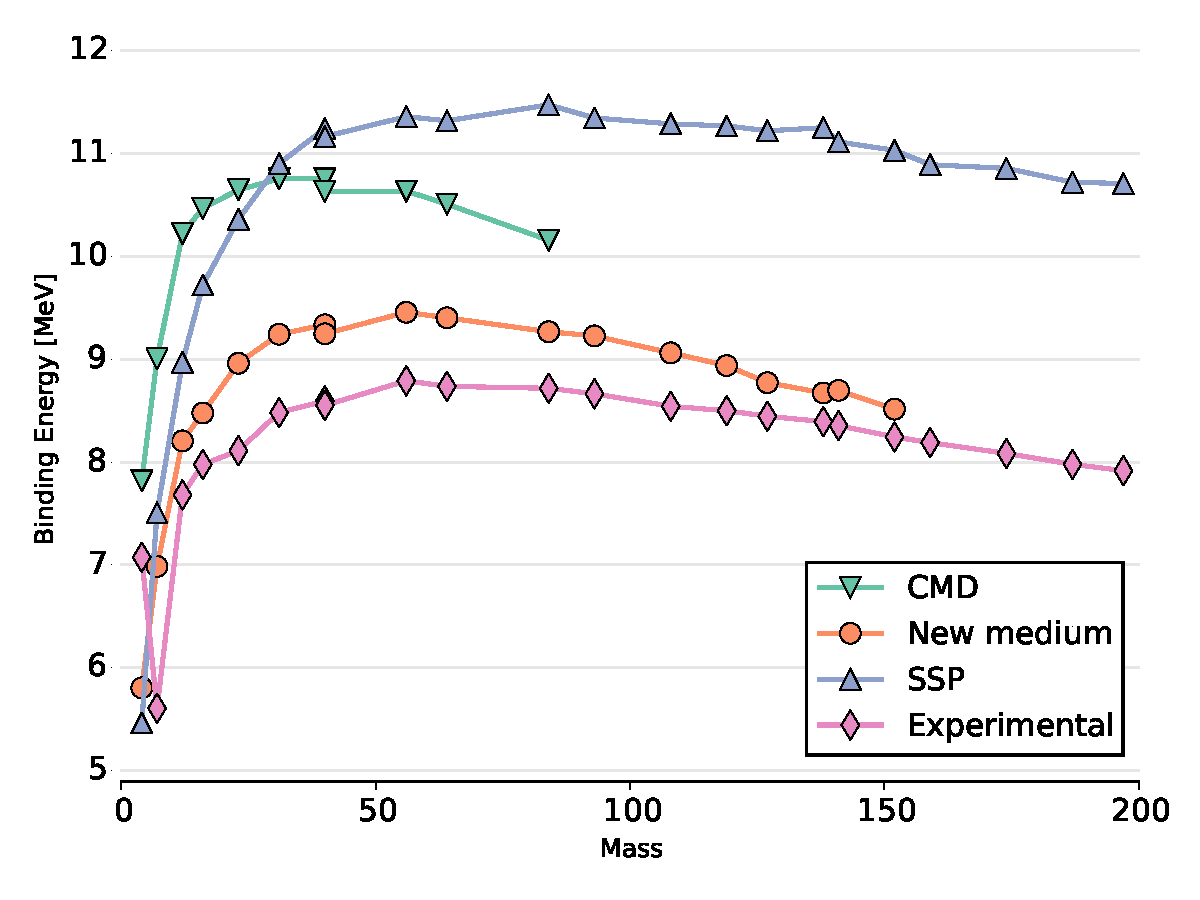
\includegraphics[width=0.8\columnwidth]{introduccion/binding}
  \caption{Binding energies of ground-state nuclei obtained with CMD
    model, extracted from Ref.~\cite{dorso_isoscaling_2011}.}
  \label{fig:binding}
\end{figure}

\subsubsection{Collisions}
With respect to collisions, these potentials are known to reproduce
nucleon-nucleon cross sections from low to intermediate
energies~\cite{lenk_accuracy_1990}, and it has been used extensively
in studying heavy ion collisions (see
Ref.~\cite{chernomoretz_quasiclassical_2002, barranon_time_2007}). For
such reactions, two ``nuclei'' are boosted against each other at a
desired energy. From collision to collision, the projectile and target
are rotated with respect to each other at random values of the Euler
angles. The evolution of the system is followed using a
velocity-Verlet algorithm with energy conservation better than 0.01\%.
At any point in time, the nucleon information, i.e., position and
momenta, can be turned into fragment information by identifying the
clusters and free particles; several such cluster recognition
algorithms have been developed by our collaborator, C.O. Dorso, and
they are well described in the
literature~\cite{dorso_when_1995,strachan_time_1997}.

The method yields mass multiplicities, momenta, excitation energies,
secondary decay yields, etc. comparable to experimental
data~\cite{belkacem_searching_1996,chernomoretz_quasiclassical_2002}.
Figure~\ref{fig:distribution}, for instance, shows experimental and
simulated parallel velocity distributions for particles obtained from
mid-peripheral and peripheral ${}^{58}Ni+C$ collisions performed at
the Coupled Tandem and Super-Conducting Cyclotron accelerators of AECL
at Chalk River~\cite{chernomoretz_quasiclassical_2002}.

\begin{figure}[h]
  \begin{subfigure}[h!]{\columnwidth}
    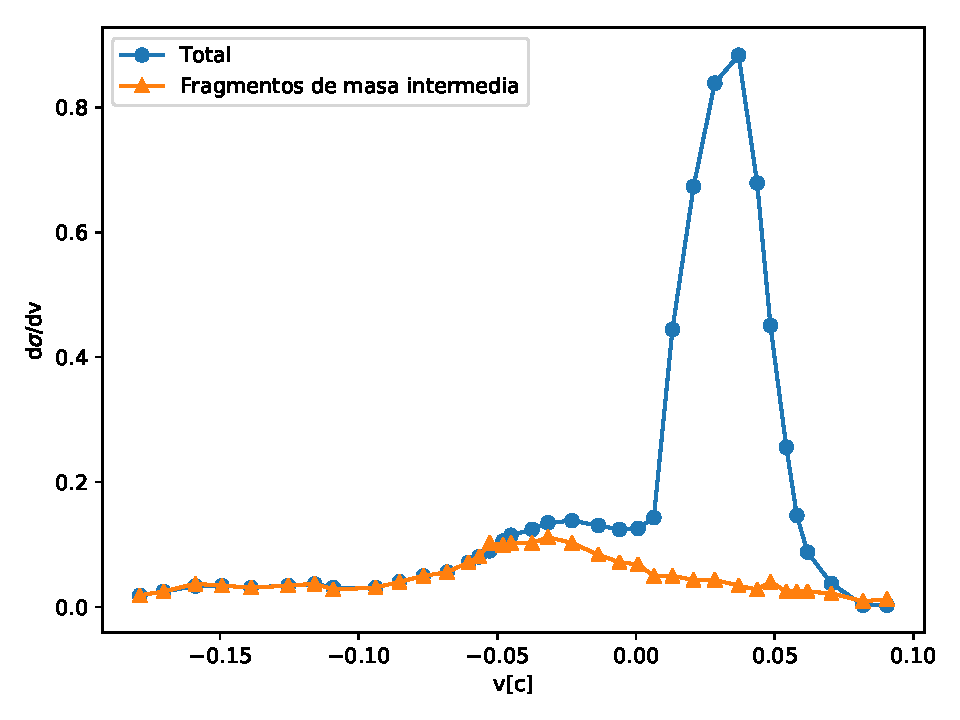
\includegraphics[width=\columnwidth]{introduccion/cherno_experiment}
    \caption{$\eta = 0.0001\,\text{fm/c}$}
    \label{sfig:exp}
  \end{subfigure}
  \begin{subfigure}[h!]{\columnwidth}
    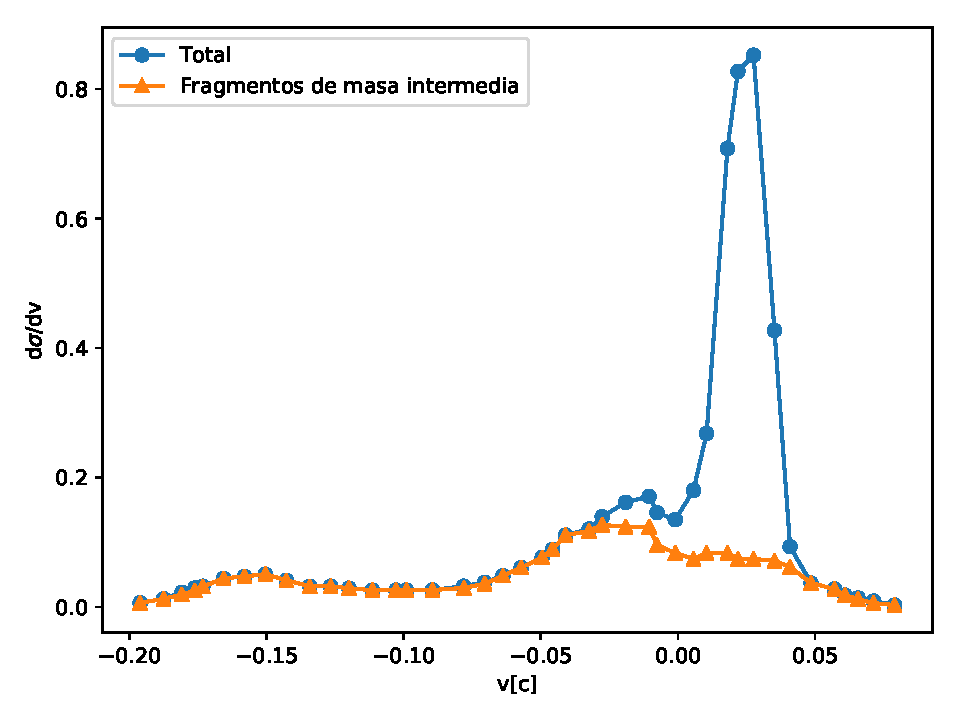
\includegraphics[width=\columnwidth]{introduccion/cherno_simulation}
    \caption{$\eta = 0.0001\,\text{fm/c}$}
    \label{sfig:sim}
  \end{subfigure}
  \centering
  \caption{\ref{sfig:exp} Experimental and \ref{sfig:sim} simulated
    parallel velocity distributions for ${}^{58}Ni+C$ collisions.}
  \label{fig:distribution}
\end{figure}


\subsubsection{Thermostatic Properties of Nuclear Matter} To study
thermal properties of static nuclear matter, these drops or infinite
systems, nucleons are positioned at random, but with a selected
density, in a container and ``heated". After equilibration, the system
can then be used to extract macroscopic variables. Repeating these
simulations for a wide range of density and temperature values,
information about the energy per nucleon, $\epsilon(\rho,T)$, can be
obtained and used to construct analytical fits in the spirit of those
pioneered by Bertsch, Siemens, and Kapusta~\cite{bertsch_nuclear_1983,
  kapusta_deuteron_1984, lopez_nuclear_1984}; these fits in turn can
be used to derive other thermodynamic variables, such as pressure,
etc.

Figure~\ref{fig:energy_nm} shows the results of the method as applied
by Gim\'enez-Molinelli \emph{et
  al.}~\cite{gimenez_molinelli_simulations_2014} for stiff cold
infinite nuclear matter. The open symbols correspond to CMD
calculations at low temperatures, showing a departure from the imposed
homogeneous solutions obtained with the full symbols for different
crystal symmetries. This shows the emergence of pseudo pastas in
nuclear matter.

For finite systems, figure~\ref{fig:caloric} demonstrates the
feasibility of using CMD to study thermal properties such as the
caloric curve (i.e. the temperature - excitation energy relationship)
for a system of 80 nucleons equilibrated at four different densities;
see Ref.~\cite{dorso_isoscaling_2011} for complete details.

\begin{figure}[h]
  \centering
  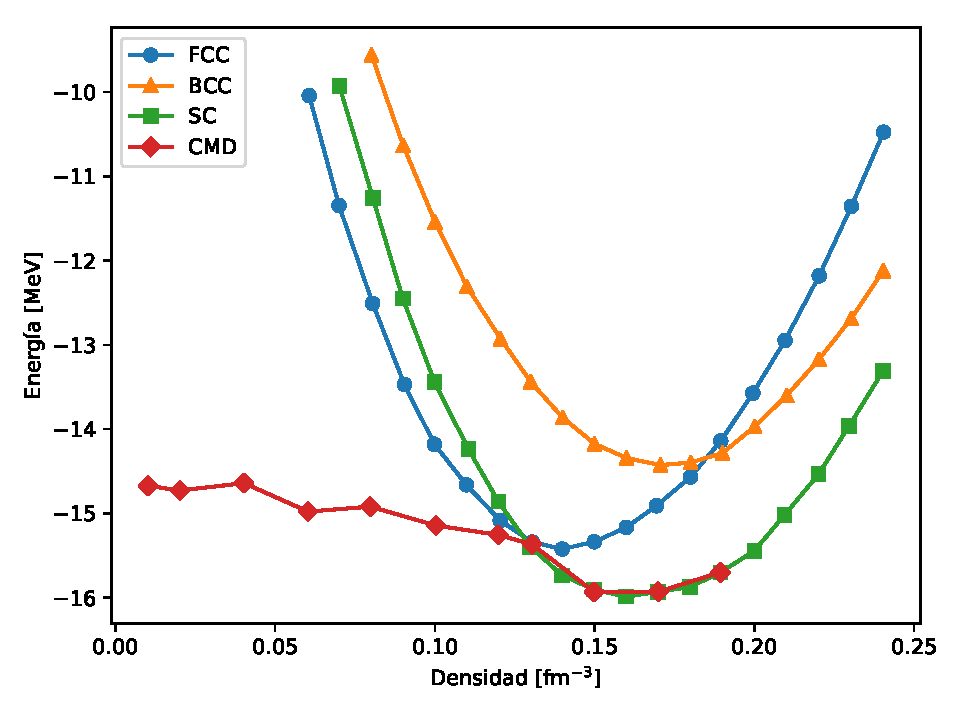
\includegraphics[width=\columnwidth]{introduccion/energy_nm}
  \caption{Nuclear matter energy per particle of cold matter
    calculated with CMD. Full symbols are for homogeneous systems,
    while open circles denote the emergence of the pseudo-pasta.}
  \label{fig:energy_nm}
\end{figure}


\begin{figure}[h]
  \centering
  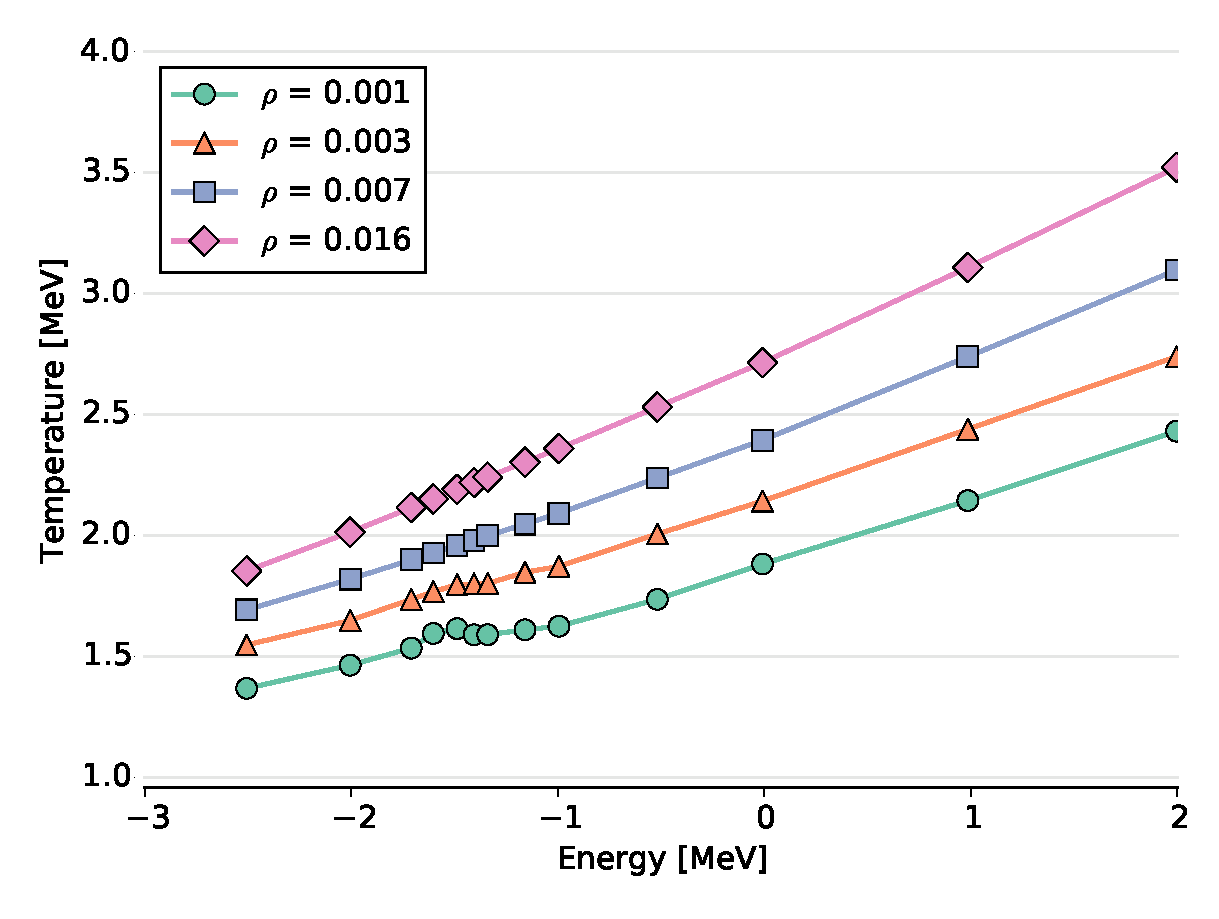
\includegraphics[width=\columnwidth]{introduccion/caloric}
  \caption{Caloric curve of a system equilibrated at four different
    densities calculated with CMD.}
  \label{fig:caloric}
\end{figure}


\subsection{Coulomb interaction in the model}\label{sc:coulomb}

Since a neutralizing electron gas embeds the nucleons in the neutron
star crust, the Coulomb forces among protons are screened. The model
we used to model this screening effect is the Thomas-Fermi
approximation, used with various nuclear
models~\cite{maruyama_quantum_1998, dorso_topological_2012,
  horowitz_neutrino-pasta_2004}. According to this approximation,
protons interact via a Yukawa-like potential, with a screening length
$\lambda$:
\begin{equation*}
 V_{TF}(r) = q^2\frac{e^{-r/\lambda}}{r}.
\end{equation*}

Theoretical estimates for the screening length $\lambda$ are
$\lambda\sim100\,\text{fm}$~\cite{fetter_quantum_2003}, but we set the
screening length to $\lambda=20\,\text{fm}$. This choice was based on
previous studies~\cite{alcain_effect_2014}, where we have shown that
this value is enough to adequately reproduce the expected length scale
of density fluctuations for this model, while larger screening lengths
would be a computational difficulty. We analyze the opacity to
neutrinos of the structures for different proton fractions and
densities.

\section{Neutron Star Matter at low densities and
  temperature}\label{sc:nsm_lowd}

When we consider the system with a screened Coulomb interaction as
described in~\ref{sc:coulomb}, a very interesting phenomena takes
place, described with detail in Ref.~\cite{alcain_effect_2014}. At
sub-saturation densities, the system displays an inhomogeneous
structure known as nuclear pasta, characterized by the emergence of
multiple structure per simulation cell, that can be roughly classified
as \emph{gnocchi}, \emph{spaghetti}, \emph{lasagna} and tunnels. As an
example, in figure~\ref{fig:pasta} we show the configurations of some
of these pastas.


\begin{figure}[h]
  \begin{subfigure}[h!]{0.45\columnwidth}
    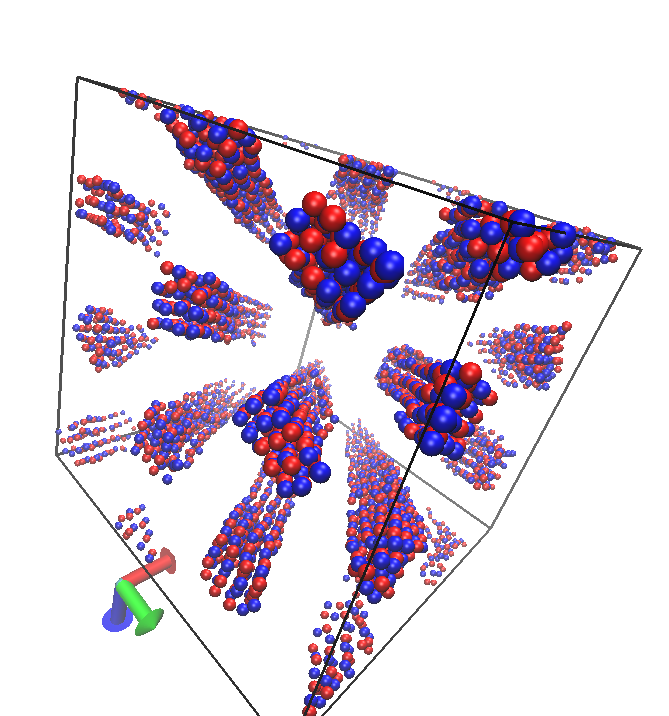
\includegraphics[width=\columnwidth]{introduccion/spaghetti}
    \caption{$\rho = 0.03\,\text{fm}^{-3}$}
    \label{sfig:spaghetti}
  \end{subfigure}
  \begin{subfigure}[h!]{0.45\columnwidth}
    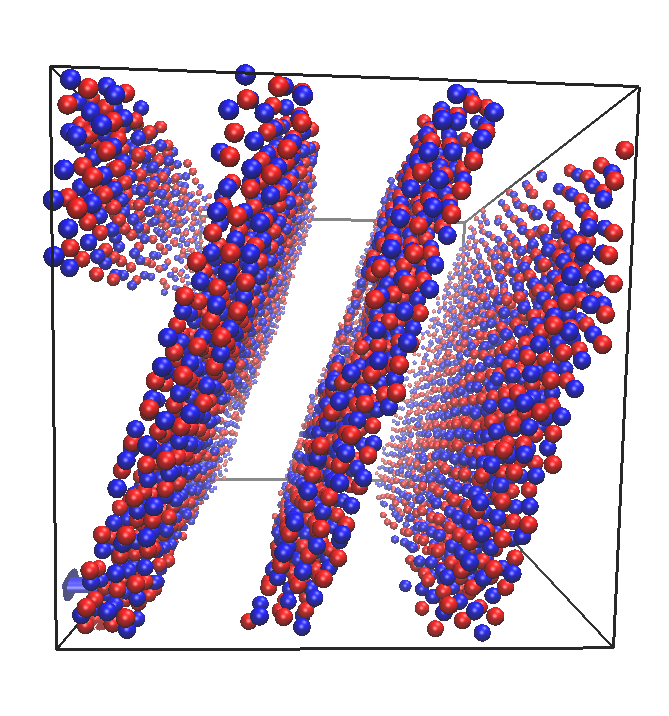
\includegraphics[width=\columnwidth]{introduccion/lasagna}
    \caption{$\rho = 0.05\,\text{fm}^{-3}$}
    \label{sfig:lasagna}
  \end{subfigure}
  \begin{subfigure}[h!]{0.45\columnwidth}
    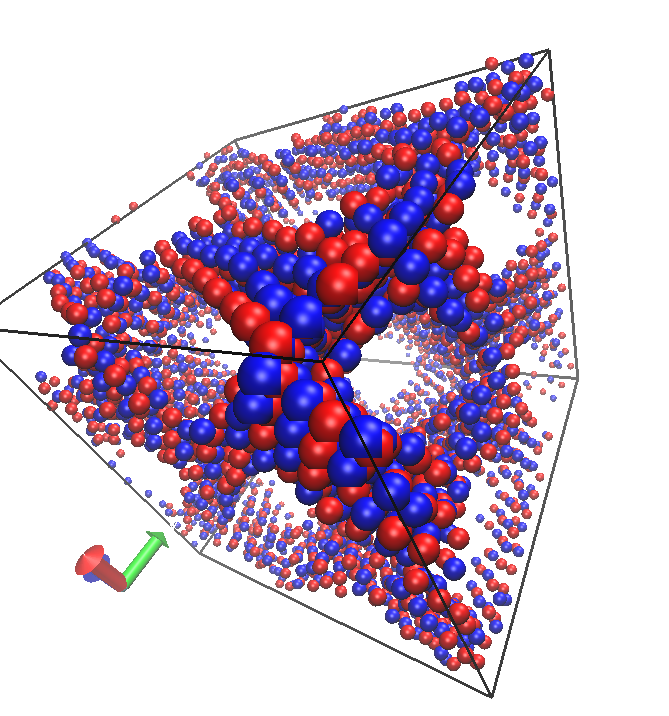
\includegraphics[width=\columnwidth]{introduccion/tunnels}
    \caption{$\rho = 0.08\,\text{fm}^{-3}$}
    \label{sfig:tunnels}
  \end{subfigure}
  \centering
  \caption{\ref{sfig:spaghetti} Spaghetti, \ref{sfig:lasagna} lasagna
    and \ref{sfig:tunnels} tunnels obtained with the CMD method, for
    the symmetric case $x=0.5$ and low temperature $T=0.5\,\text{MeV}$
    extracted from Ref.~\cite{alcain_effect_2014}}
  \label{fig:pasta}
\end{figure}


\section{Expansion}\label{sc:expansion}

To simulate an expanding system we scale linearly with time the length
of the box in every dimension,
\begin{equation*}
  L(t) = L_0 (1 + \eta\,t)
\end{equation*}
This, however, is not enough to expand the system collectively. We
also need the particles inside the cell to expand like the box. In
order to accomplish this, based on Ref.~\cite{dorso_onset_1996}, we
add to each particle a velocity $v_{exp}$ dependent on the position in
the box:
\begin{equation*}
  \mathbf{v_{exp}} = \eta\,\mathbf{r}
\end{equation*}
We can see from this expression that the particles in the edge of the
box will have an expanding velocity equal to that of the box.

Another effect to consider of this expansion is that when a particle
crosses a boundary its velocity has to change according to the
velocity of the expanding box. For example, if the particle crosses
the left-hand boundary of the periodic box, the velocity of the image
particle $v_i^\dagger$ on the right-hand must be modified $v_i^\dagger
= v_i + L_0\,\eta$.

\section{Cluster recognition}\label{sc:cluster}
In typical configurations we have not only the structure known as
nuclear pasta, but also a nucleon gas that surrounds the nuclear
pasta. In order to properly characterize the pasta phases, we must
know which particles belong to the pasta phases and which belong to
this gas. To do so, we have to find the clusters that are formed along
the simulation.

One of the algorithms to identify cluster formation is Minimum
Spanning Tree (MST). In MST algorithm, two particles belong to the
same cluster $\{C^{\text{MST}}_n\}$ if the relative distance of the
particles is less than a cutoff distance $r_{cut}$:
\begin{equation*}
  i \in C^{\text{MST}}_n \Leftrightarrow \exists j \in C_n \mid
  r_{ij} < r_{cut}
\end{equation*}

This cluster definition works correctly for systems with no kinetic
energy, and it is based in the attractive tail of the nuclear
interaction. However, if the particles have a non-zero temperature, we
can have a situation of two particles that are closer than the cutoff
radius, but with a large relative kinetic energy.

To deal with situations of non-zero temperatures, we need to take into
account the relative momentum among particles. One of the most
sophisticated methods to accomplish this is the Early Cluster
Recognition Algorithm (ECRA)~\cite{dorso_early_1993}. In this
algorithm, the particles are partitioned in different disjoint
clusters $C^{\text{ECRA}}_n$, with the total energy in each cluster:
\begin{equation*}
  \epsilon_n = \sum_{i \in C_n} K^{CM}_i +  \sum_{i,j \in C_n} V_{ij}
\end{equation*}
where $K^{CM}_i$ is the kinetic energy relative to the center of mass
of the cluster. The set of clusters $\{C_n\}$ then is the one that
minimizes the sum of all the cluster energies $E_{\text{partition}} =
\sum_n \epsilon_n$.

ECRA algorithm can be easily used for small
systems~\cite{dorso_fluctuation_1994}, but being a combinatorial
optimization, it cannot be used in large systems. While finding ECRA
clusters is very expensive computationally, using simply MST clusters
can give extremely biased results towards large clusters. We have
decided to go for a middle ground choice, the Minimum Spanning Tree
Energy (MSTE) algorithm~\cite{dorso_topological_2012}. This algorithm
is a modification of MST, taking into account the kinetic
energy. According to MSTE, two particles belong to the same cluster
$\{C^{\text{MSTE}}_n\}$ if they are energy bound:
\begin{equation*}
  i \in C^{\text{MSTE}}_n \Leftrightarrow \exists j \in C_n :
  V_{ij}+ K_{ij} \le 0
\end{equation*}
While this algorithm doesn't yield the same theoretically sound
results from ECRA, it still avoids the largest pitfall of naïve MST
implementations for the temperatures used in this work.

\subsection{Infinite Clusters}
We developed an algorithm for the recognition of infinite clusters
across the boundaries. We explain here in detail the implementation
for MST clusters in 2D, being the MSTE and 3D extension
straightforward. In figure~\ref{fig:scheme_clusters} we see a
schematical representation of 2D clusters recognized in a periodic
cell, labeled from 1 to 6 (note that these clusters don't connect yet
through the periodic walls).

\begin{figure}  \centering
  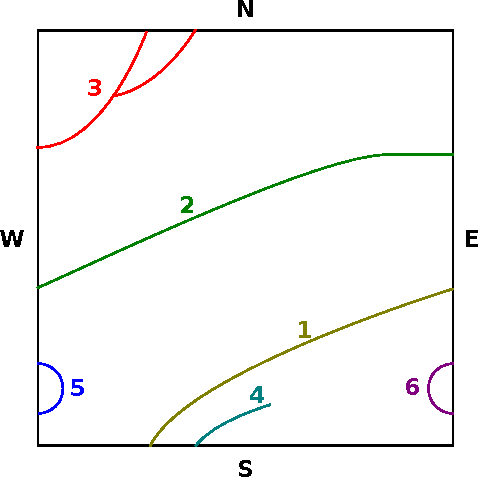
\includegraphics[width=0.75\columnwidth]{introduccion/scheme_clusters}
  \caption{(Color online) Schematical representation of 2D clusters, recognized only
    in the cell and not through the periodic walls, labeled as N, S,
    W, E. The clusters inside the cell are labeled from 1 to 6,}
\label{fig:scheme_clusters}
\end{figure}

In order to find the connections of these clusters through the
boundaries, we draw a labeled graph of the clusters, where we connect
clusters depending on whether they connect or not through a wall and
label such connection with the wall label. For example, we begin with
cluster 1. It connects with cluster 2 going out through the E wall,
therefore we add a $1\rightarrow2$ connection labeled as
E. Symmetrically, we add a $2\rightarrow1$ connection labeled as W. Now
we go for the pair 1-3. It connects going out through the S wall, so
we add $1\rightarrow3$ labeled as S and $3\rightarrow1$ labeled as
N. Cluster 1 does not connect with 4, 5, or 6, therefore those are the
only connections we have. Once we've done that, we get the graph of
figure~\ref{fig:graph_clusters}.

\begin{figure}  \centering
  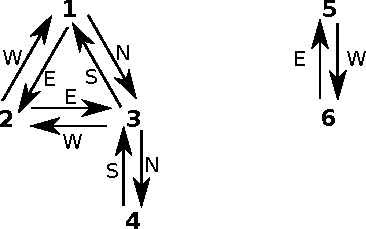
\includegraphics[width=0.45\columnwidth]{introduccion/graph_clusters}
  \caption{Graph of the clusters with connections labeled by the wall
    of the boundary they connect through. The graph can be divided in
    2 subgraphs that don't connect: 1--2--3--4 and 5--6. Each of these
    subgraphs is as cluster when periodic boundary conditions are
    considered.}
\label{fig:graph_clusters}
\end{figure}

We now wonder whether these subgraphs represent an infinite cluster or
not not. In order to have an infinite clusters, we need to have a loop
(the opposite is not true: having a loop is not enough to have an
infinite cluster, as we can see in subragph 5--6), so we first
identify loops and mark them as candidates for infinite
clusters. Every connection adds to a loop (since the graph connections
are back and forth), but we know from inspecting the
figure~\ref{fig:graph_clusters} that the cluster 1--2--3 is
infinite. Finding out what makes, in the graph, the cluster 1--2--3
infinite is key to identify infinite clusters. And the key feature of
cluster 1--2--3 is that its loop 1--2--3--1 can be transversed through
the walls E--E--S, while loops like 5--6 can be transversed only
through E--W. Now, in order for the cluster to be infinite, we need it
to extend infinitely in (at least) one direction. So once we have the
list of walls of the loop, we create a magnitude I associated to each
loop that is created as follows: beginning with $I = 0$, we add a
value $M_i$ if there is (at least one) $i$ wall. The values are: $M_E
= 1$, $M_W = -1$, $M_N = 2$, $M_S = -2$. If $I$ is nonzero, then the
loop is infinite. For example, for the loop E--E--S, we have E and S
walls, so $I = M_E + M_S = 3$ and the loop is infinite. For the loop
E--W, $I = M_E + M_W = 0$, and the loop is finite.


\chapter[Efecto de Coulomb]{Interacción de Coulomb}
\label{ch:coulomb}
En este capítulo estudiamos el rol de la interacción de Coulomb en la dinámica de los nucleones en las condiciones de la corteza de las estrellas de neutrones.
Estudiamos la materia simétrica en sisospin a densidades de sub-saturación y temperaturas bajas.
La interacción electrostática entre protones es incluida como un potencial de Coulomb apantallado, en el espíritu de la aproximación de Thomas-Fermi, pero variando artificialmente la longitud de apantallamiento para estudiar su efecto en la formación de las estructuras nuclears no homogéneas conocidas como ``pasta nuclear''.
A medida que aumenta la longitud de apantallamiento, podemos ver una transición de un régimen de una pasta por celda (debido exclusivamente a efectos de tamaño finito) a un régimen en el que aparecen múltiples pastas por celda.
Esta diferencia cualitativa en la estructura de la materia de estrellas de neutrones a bajas temperaturas muestra que se debe tomar especial cuidado cuando la longitud de apantallamiento es estimada para simulaciones numéricas.

Como observamos en trabajos previos~\cite{schneider_nuclear_2013,gimenez_molinelli_simulations_2014}, en ausencia de la interacción de Coulomb (equivalente a $\lambda=0$), estructuras tipo pastas pueden ser observadas, aunque sólo una por celda.
Estas \emph{pseudo-pastas} también tienen formas de esferas, tubos, placas, anti-tubos y anti-esferas, exactamente como la pasta con la interacción de Coulomb.
La mayor diferencia e sque, sin la interacción de Coulomb, encontramos siempre una estructura por celda, lo que nos hace pensar que la estructura está relacionada con la condición periódica de contorno impuesta en la caja,
La \emph{pseudo-pasta} esite debido a efectos de tamaño finito y, si la caja no existiera, la solución sería una gota infinita.
Notamos, sin embargo, que cuando existe la interacción de Coulomb, la competencia entre interacciones opuestas genera una longitud característica, ya no relacionada con el tamaño de la caja.
A densidades de sub-saturación esta competencia es responsable por las fases de pasta, y en el límite de densidades muy bajas le da forma a los nucleos a los que estamos acostumbrados.

Incrementar el valor de $\lambda$ comenzando desde $0\,\text{fm}$, apuntamos a explorar la transición de las pastas artificiales en las que se produce una estructura por celda hacia las pastas más realistas que tienen múltiples estructuras en cada celda de simulación.
Más aún, esto nos permite estudiar las implicancias físicas del valor arbitrario y utilizado tradicionalmente de $\lambda=10\,\text{fm}$.

\section{Introducción}

En las estrellas de neutrones, además de los protones y neutrones, existe un gas de electrones que permea todo el espacio.
Este gas de electrones apantalla la interacción electrostática de rango largo entre los protones.
Este efecto de apantallamiento es usualmente modelado con la aproximación de Thomas-Fermi, de acuerdo a la cual la interacción entre protones es un optencial del tipo Yukawa con una longitud de apantallamiento $\lambda$:

\begin{equation*}
 V_{TF}(r) = \text{q}^2\frac{e^{-r/\lambda}}{r}
\end{equation*}

De acuerdo a cálculos de Teoría Cuántica de Campos~\cite[pp. 175-180]{fetter_quantum_2003}, la longitud de apantallamiento a las densidades de interés es $\lambda\approx100\,\text{fm}$. 
Para simulaciones numéricas una interacción de rango tan largo implica un problema ya que, para realizar simulaciones correctas, el dominio de la simulación debería ser mayor que la longitud de los potenciales de interacción.
El valor correcto de $\lambda$ requeriría trabajar con $\approx 10^6$ partículas, y sería muy complicado de realizar computacionalmente.
Al enfrentar este inconveniente, distintos autores~\cite{maruyama_molecular_2012, horowitz_neutrino-pasta_2004} decidieron trabajar con un valor mucho menor $\lambda=10\,\text{fm}$, con la esperanza de retener los principales aspectos cualitativos y fenomenológicos del sistema (interacciones competitivas de distinto rango) al trabajar con sistemas más pequeños.
Incluso si fueran capaces de producir estructura del tipo pasta, la elección particular del valor para la longitud de apantallamiento es arbitraria y basada casi únicamente end etalles computacionales.
Notablemente, este valor de longitud de apantallamiento fue utilizado
consecutivamente por los autores desde ese momento~\cite{maruyama_quantum_1998, horowitz_neutrino-pasta_2004, dorso_topological_2012}.
En este capítulo nos centraremos en el estudio de las consecuencias física de esta elección arbitraria.

El rol de la longitud de apantallamiento ha sido apenas explorado en otros modelos.
Por ejemplo, en un estudio del 2003~\cite{watanabe_electron_2003}, el efecto de apantallamiento de un gas de electrones en estructuras nucleares fue investigado utilizando un modelo estático de gota líquida.
En este estudio se encontró que el principal efecto del gas apantallante fue extender el ragno de densidades en las que las burbujas y los fragmentos aparecían, y reducir el ragno de estabilidad de fases homogéneas.
A pesar de que la relevancia del apantallamiento resultó menor, el estudio, al ser estático, no incluía ningún efeco dinámico.

Otro estudio, del 2005~\cite{maruyama_nuclear_2005}, utilizó una funcional densidad para investigar el apantallamiento de la carga en estructuras nucleares a densidades menores a la nuclear, pero a temperatura cero; en particular se compararon casos con y sin apantallamiento.
Los resultados principales del estudio fueron perfiles de densidad de nucleones utilizadeos para cuantificar el ordenamiento de las densidades de carga de protones y electrones.
Nuevamente, hallaron que las regiones de densidad en las que existe la pasta se amplían cuando se considera el apantallamiento de Coulomb, especialmente debido al reordenamiento de los protones; los autores remarcan la importancia de extender este estudio a temperaturas finitas y con modelos dinámicos.

Más recientemente, algunos trabajos~\cite{schneider_nuclear_2013,gimenez_molinelli_simulations_2014} comenzaron a estudiar el efecto que tiene la interacción de Coulomb en la formación de pasta utilizando modelos dinámicos.
Los hallazgos principales fueron que la pasta artificial, de una estructura por celda (\emph{pseudo-pasta}), podía existir incluso en ausencia de interacción de Coulomb, y que existía debido a las condiciones periódicas de contorno y el tamaño finito~\cite{binder_beyond_2012}.

\section{Longitud de apantallamiento ``crítica''}\label{lambda_c}

Una forma de analizar la naturaleza de la pasta obtenida es a través de la presión de las distintas configuraciones.

Podemos medir la presión a través de la fórmula del virial
\begin{equation*}
P=\frac{N\,k_B\,T}{V} + \frac{1}{3}
\frac{\Sigma_{i}^{N}\mathbf{r}_i\cdot\mathbf{F}_i}{V}
\end{equation*}
donde $N$ es el número de partículas en el sistema y $\mathbf{F}$ la fuera ejercida sobre cada nucleón.
Los términos en la fórmula del virial se aplican sólo a las interacciones epecíficas del modelo, sin contemplar la presión del gas de electrones.
Esta presión no debe ser confundida con la presión esperada en la corteza de las estrellas de neutrones (ya que los electrones deberían ser considerados explícitamente para calcularla adecuadamente), sino simplemente una prueba de la estabilidad mecánica de las configuraciones obtenidas con este modelo.
En la figura~\ref{fig:pre} vemos que para todo $\lambda<10\,\text{fm}$ la presión es negativa.

La presión negativa es una señal de que las estructuras no-homogéneas encontradas son artificiales, y que las estructuras sólo pueden existir bajo condiciones periódicas de contorno (ver~\cite{binder_beyond_2012,gimenez_molinelli_simulations_2014}).
Podemos pensar al sistema como la celda primitiva de la simulación bajo la tensión causada por sus réplicas periódicas.
Esto significa que, para longitudes de apantallamiento tan bajas, la interacción efectiva es atractiva y las condiciones periódicas de contorno todavía juegan un rol importante en la forma del estado de mínima energía.

Para $\lambda>10\,\text{fm}$ la presión se vuelve positiva, lo que quiere decir que las estructuras que se forman en estas configuraciones no se deben sólo a las condiciones periódicas de contorno, sino que la interacción de Coulomb está comenzando a jugar un rol.
Las configuraciones para estos valores de $\lambda$ muestran efectivamente fluctuaciones de densidad de longitud menor que el tamaño de la caja, que sólo pueden ser atribuidas a la competencia entre el término de Coulomb y el término nuclear.
Sin embargo, la forma de las estructuras, caracterizadas a través de las funcionales de Minkowski, cambia drásticamente con $\lambda$.

\begin{figure}[h!]  \centering
\centering
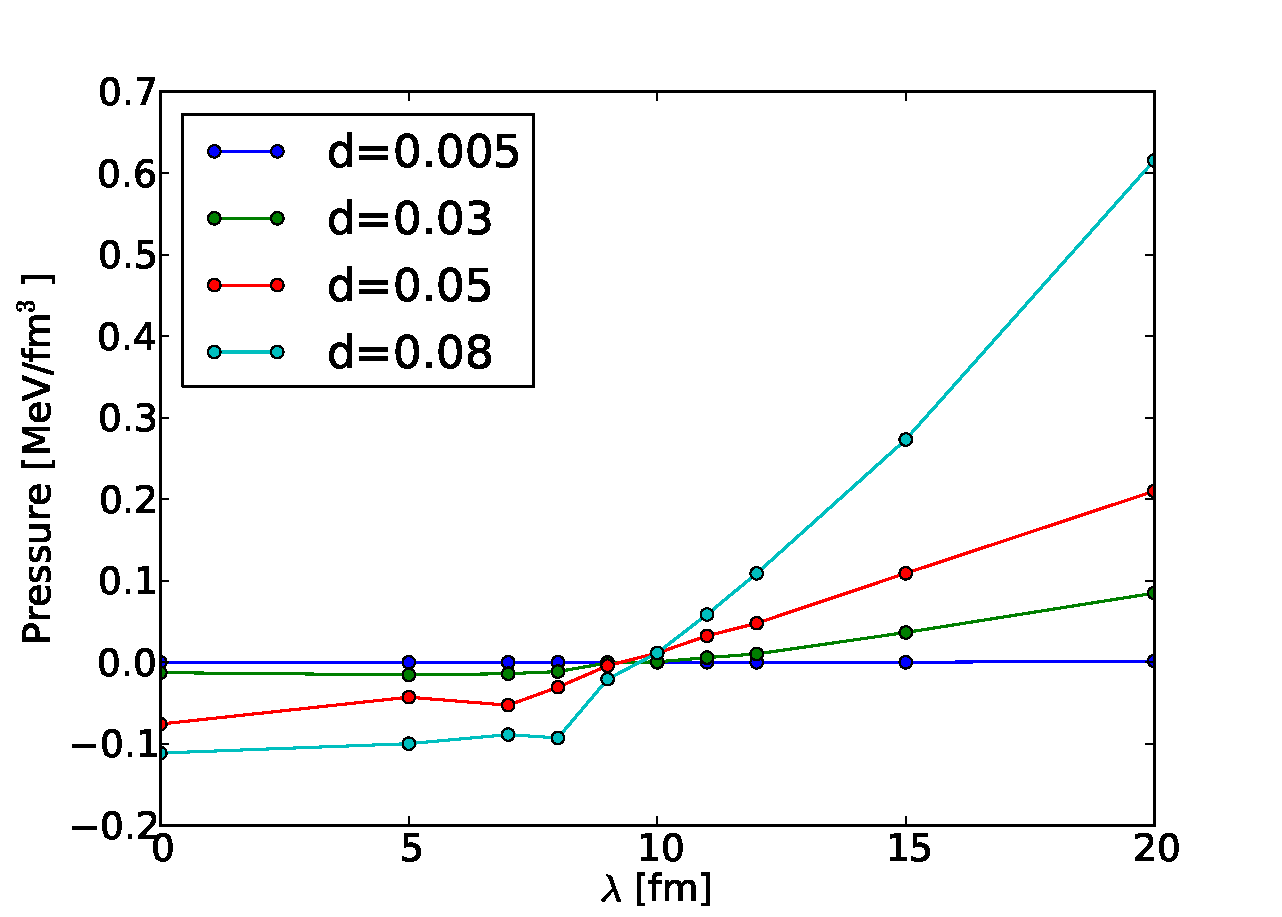
\includegraphics[width=0.4\columnwidth]{coulomb/pre.pdf}
\caption{Presión como función del apantallamiento $\lambda$ para distintas densidades.
  Podemos ver que para $\lambda<10\,\text{fm}$ la presión es negativa, sugiriendo que las condiciones periódicas de contorno están afectando la morfología de la solución.}
\label{fig:pre}
\end{figure}

Para clasificar las estructuras de bajas temperaturas ($T=0.001\,\text{MeV}$) para cada valor de $\lambda$, estudiamos su morfología con las herramientas de análisis para la distribución espacial de partículas: las funcionales de Minkowski.
En las figuras~\ref{fig:minkowski} podemos ver la superficie, ancho medio y número de Euler para los estados hallados y su dependencia con $\lambda$ para distintas densidades.

\begin{figure}[h!]  %figure 5 \centering
\centering
\begin{subfigure}[h!]{0.4\columnwidth}
  \centering
  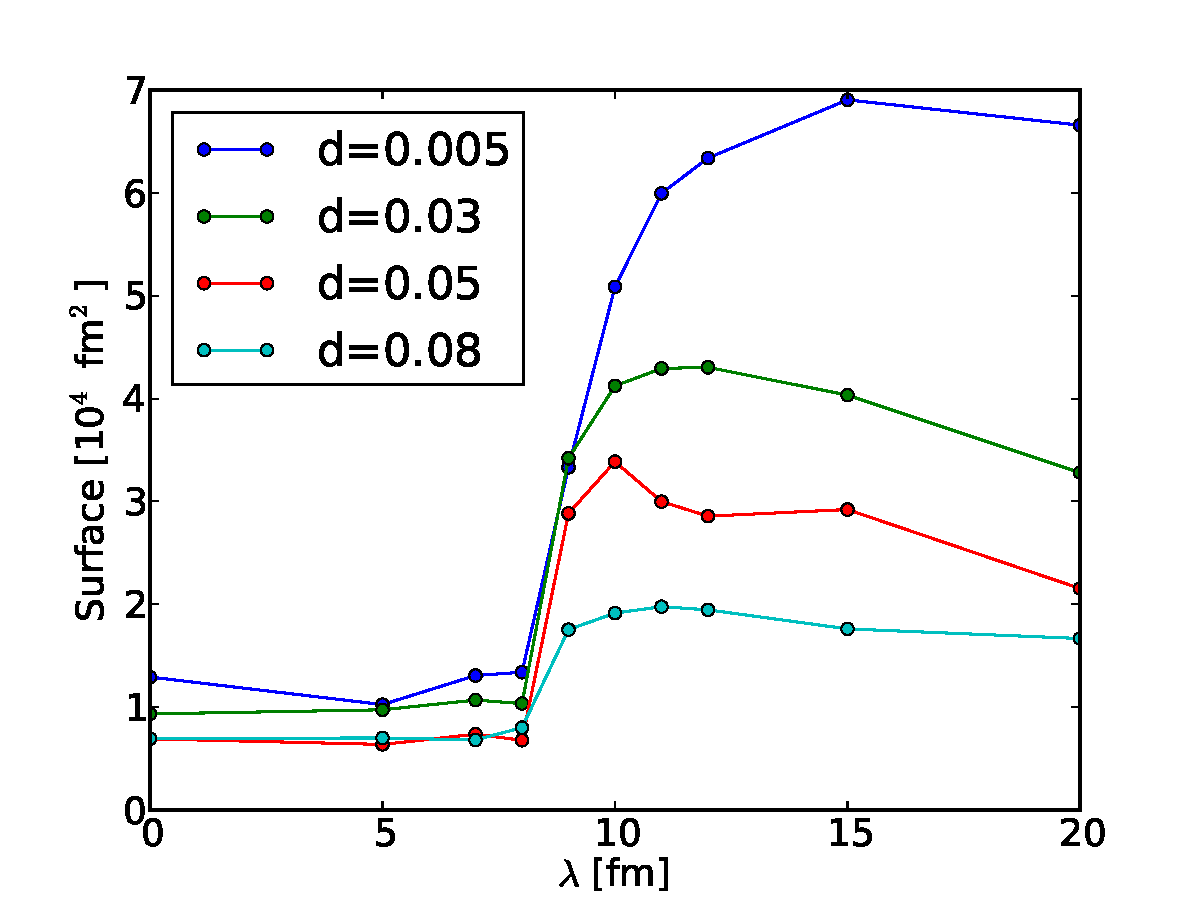
\includegraphics[width=\columnwidth]{coulomb/sup.pdf}
  \caption{Superficie}
\end{subfigure}
\begin{subfigure}[h!]{0.4\columnwidth}
  \centering
  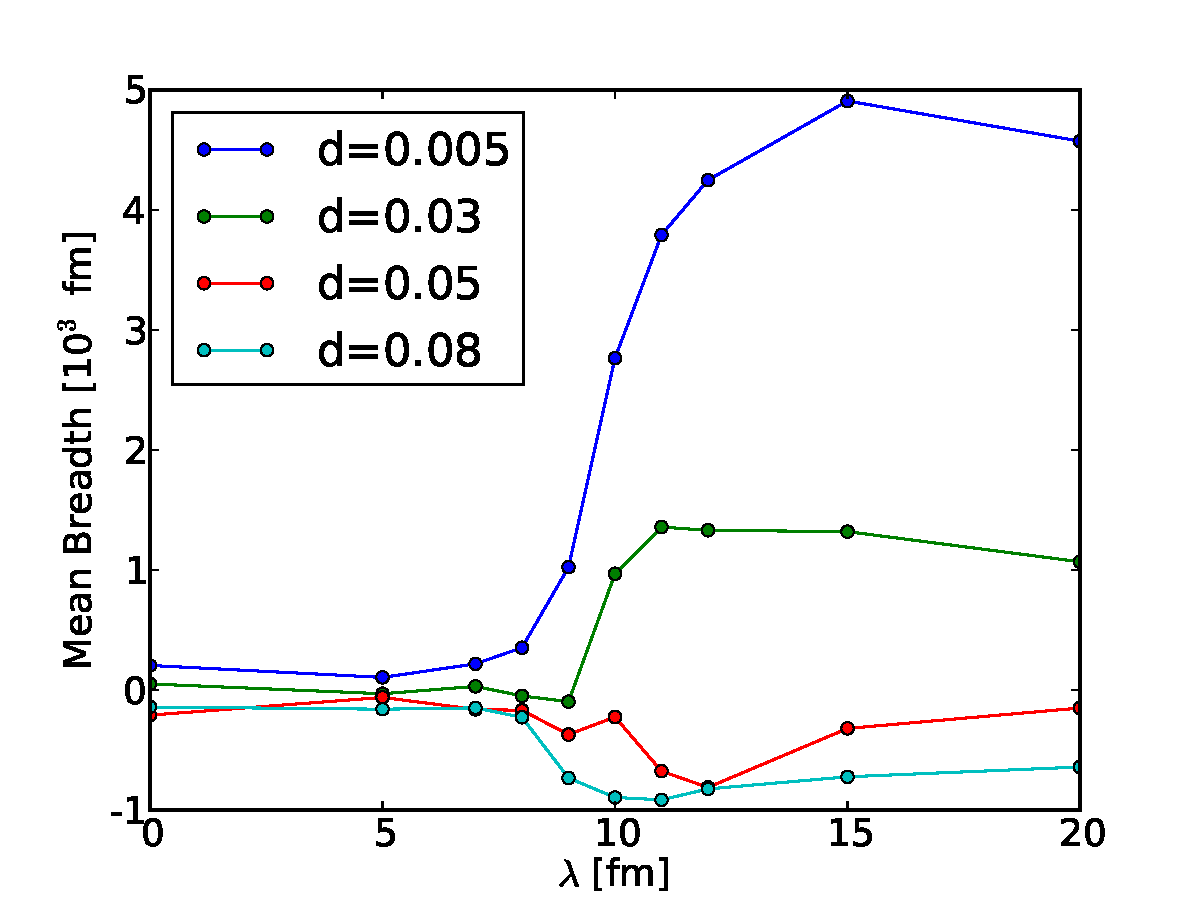
\includegraphics[width=\columnwidth]{coulomb/cur.pdf}
  \caption{Ancho medio}
\end{subfigure}
\begin{subfigure}[h!]{0.4\columnwidth}
  \centering
  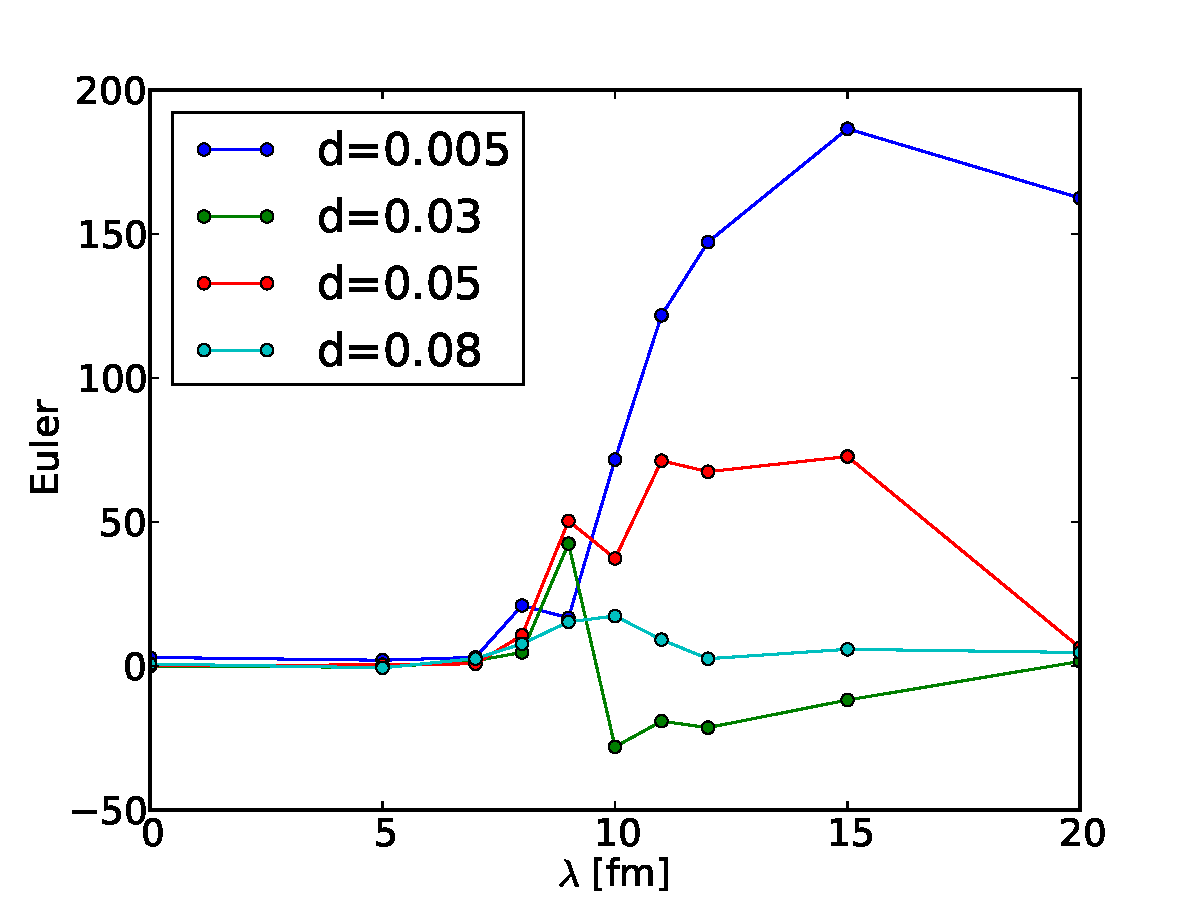
\includegraphics[width=\columnwidth]{coulomb/eul.pdf}
  \caption{Número de Euler}
\end{subfigure}
\caption{Dependencia de las funcionales de Minkowski con $\lambda$.
  Podemos observar un régimen de transición entre $\lambda=7\,\text{fm}$ y $\lambda=15\,\text{fm}$, donde las funcionales de Minkowski cambian.}
\label{fig:minkowski}
\end{figure}

\begin{table}[ht] \centering
\caption{Clasificación Ancho - Euler}
\begin{tabular}{c|| c | c | c} \hline & Ancho $<0$ & Ancho
$\sim 0$ & Ancho $>0$ \\
               
\hline\hline Euler $>0$ & Anti-Gnocchi (Burbujas) & & Gnocchi \\

Euler $\sim0$ & Anti-Spaghetti (Túneles) & Lasagna & Spaghetti \\

Euler $<0$ & Anti-Jungle Gym & & Jungle Gym \\ [1ex] \hline
\end{tabular}
\label{tab:mink}
\end{table}

Como se muestra en la tabla~\ref{tab:mink}, esperamos que \emph{lasagna} y \emph{spaghetti} tengan un número de Euler $\chi=0$.
Para el caso de los \emph{gnocchi}, sin embargo, cada uno de ellos contribuye con $\chi_{gn}=2$.
Esto significa que el número de Euler para todo el sistema de $N_{gn}$ \emph{gnocchi} será $\chi=2\cdot\,N_{gn}$.
A medida que las configuraciones se parten en múltiples estructuras por celda al aumentar $\lambda$, esperamos que también aumente la superficie.
En cuanto al ancho medio, el comportamiento descripto en la tabla~\ref{tab:mink} (positivo para \emph{spaghetti} y \emph{gnocchi}, cero para \emph{lasagna} y negativo para \emph{tunnel}) sólo se observa para $\lambda=20\,\text{fm}$.
Entre $\lambda=7\,\text{fm}$ y $\lambda=10\,\text{fm}$ las tres funcinonales de Minkowski cambian drásticamente antes de alcanzar valores bien definidos.
Esto indica que hay un régimen de transición en el que las estructuras no se pueden describir como cualquiera de las pastas tradicionales.
Para este modelo de interacción nuclear y Coulomb, parece que el valor usual de $\lambda=10\,\text{fm}$ es demasiado bajo.


\section{One vs Many} \label{pasta-bup}

\begin{figure}
\centering
\begin{subfigure}[h!]{0.5\columnwidth}
  \centering
  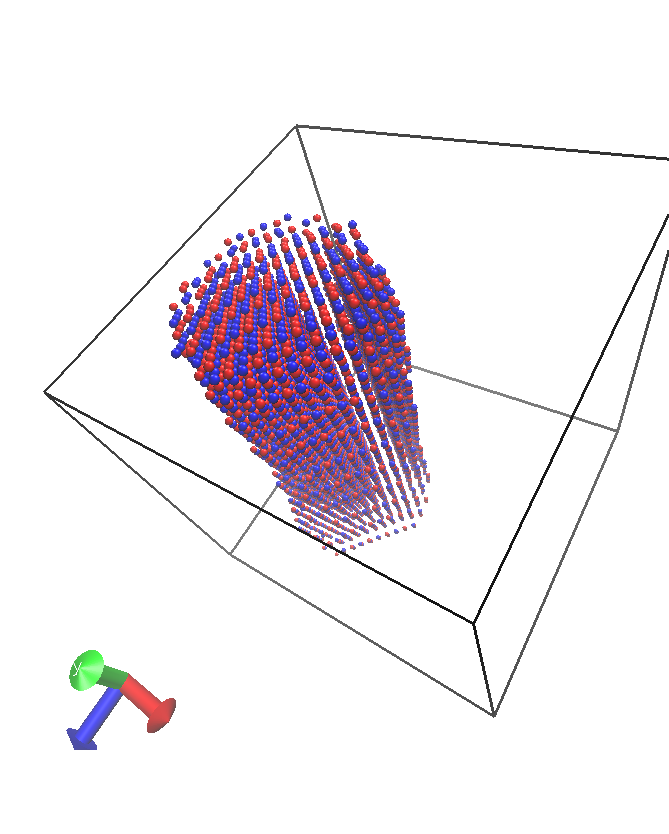
\includegraphics[width=\columnwidth]{coulomb/cou0-d0-03.png}
  \caption{$\rho=0.03\,\text{fm}^{-3}$, $\lambda=0\,\text{fm}$}
\end{subfigure}
\begin{subfigure}[h!]{0.5\columnwidth}
  \centering
  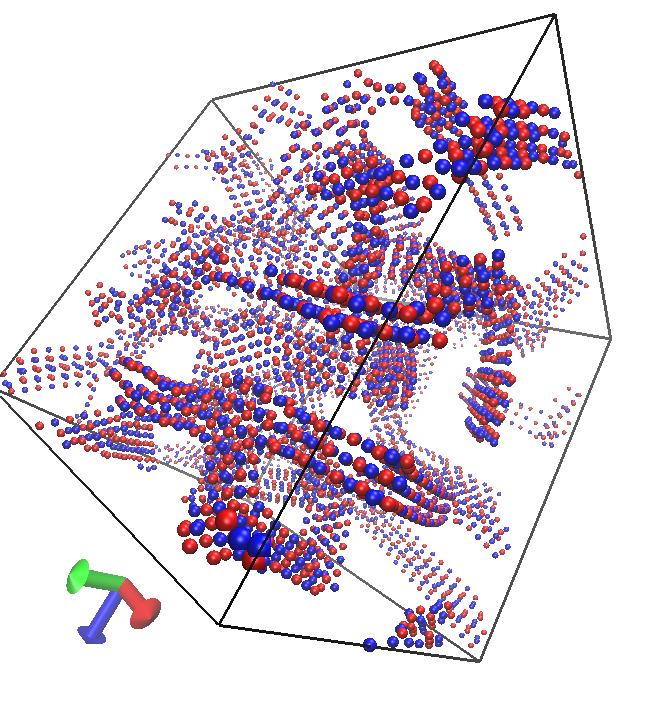
\includegraphics[width=\columnwidth]{coulomb/cou10-d0-03.png}
  \caption{$\rho=0.03\,\text{fm}^{-3}$, $\lambda=10\,\text{fm}$}
\end{subfigure}
\begin{subfigure}[h!]{0.5\columnwidth}
  \centering
  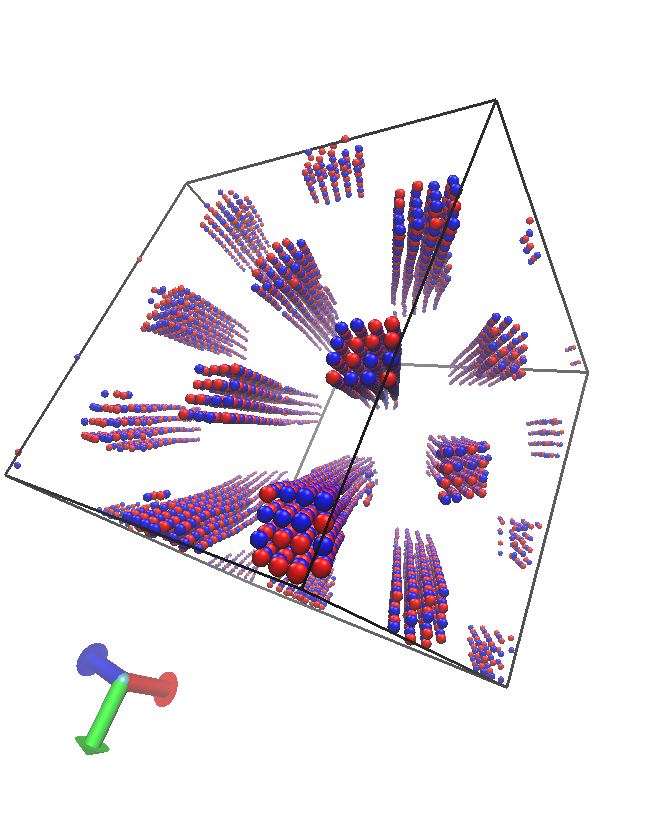
\includegraphics[width=\columnwidth]{coulomb/cou20-d0-03.png}
  \caption{$\rho=0.03\,\text{fm}^{-3}$, $\lambda=20\,\text{fm}$}
\end{subfigure}

\begin{subfigure}[h!]{0.5\columnwidth}
  \centering
  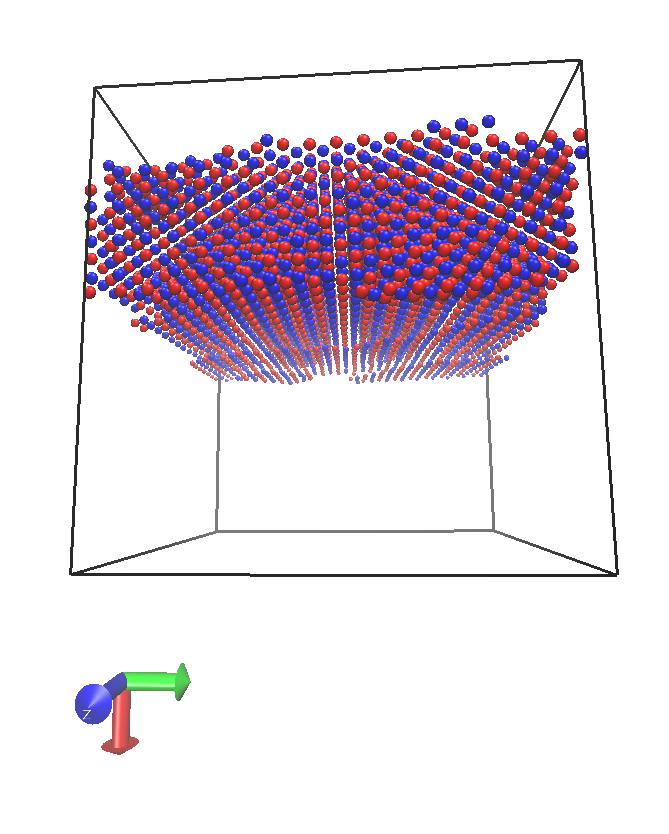
\includegraphics[width=\columnwidth]{coulomb/cou0-d0-05.png}
  \caption{$\rho=0.05\,\text{fm}^{-3}$, $\lambda=0\,\text{fm}$}
\end{subfigure}
\begin{subfigure}[h!]{0.5\columnwidth}
  \centering
  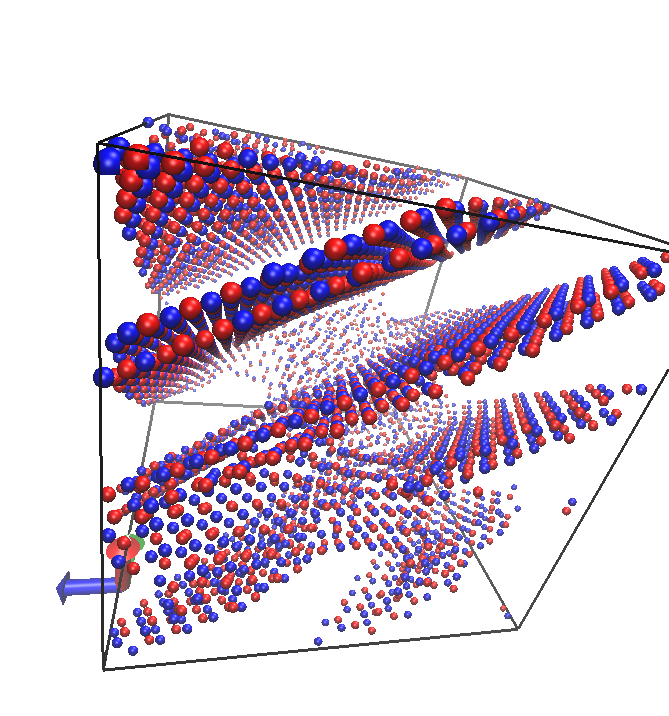
\includegraphics[width=\columnwidth]{coulomb/cou10-d0-05.png}
  \caption{$\rho=0.05\,\text{fm}^{-3}$, $\lambda=10\,\text{fm}$}
\end{subfigure}
\begin{subfigure}[h!]{0.5\columnwidth}
  \centering
  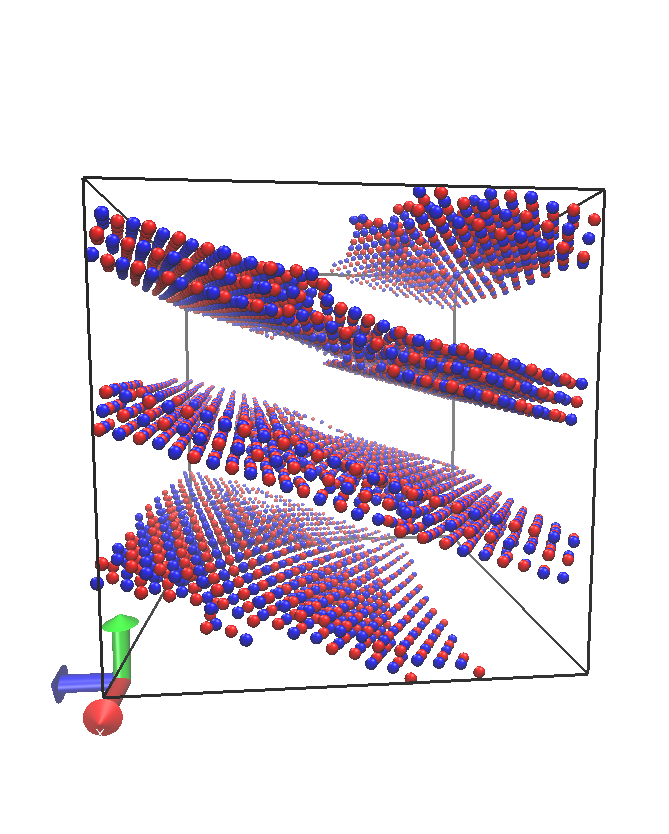
\includegraphics[width=\columnwidth]{coulomb/cou20-d0-05.png}
  \caption{$\rho=0.05\,\text{fm}^{-3}$, $\lambda=20\,\text{fm}$}
\end{subfigure}

\begin{subfigure}[h!]{0.5\columnwidth}
  \centering
  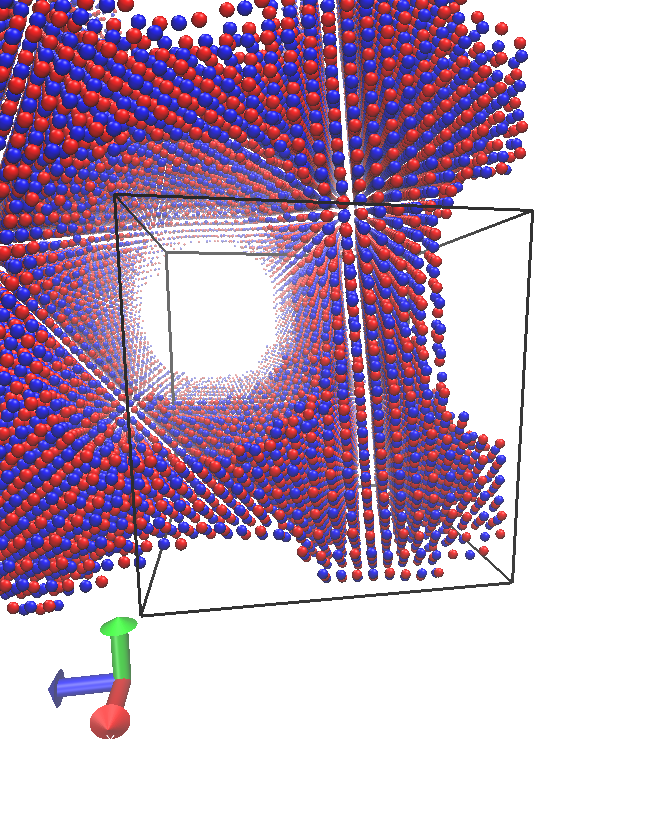
\includegraphics[width=\columnwidth]{coulomb/cou0-d0-08.png}
  \caption{$\rho=0.08\,\text{fm}^{-3}$, $\lambda=0\,\text{fm}$}
\end{subfigure}
\begin{subfigure}[h!]{0.5\columnwidth}
  \centering
  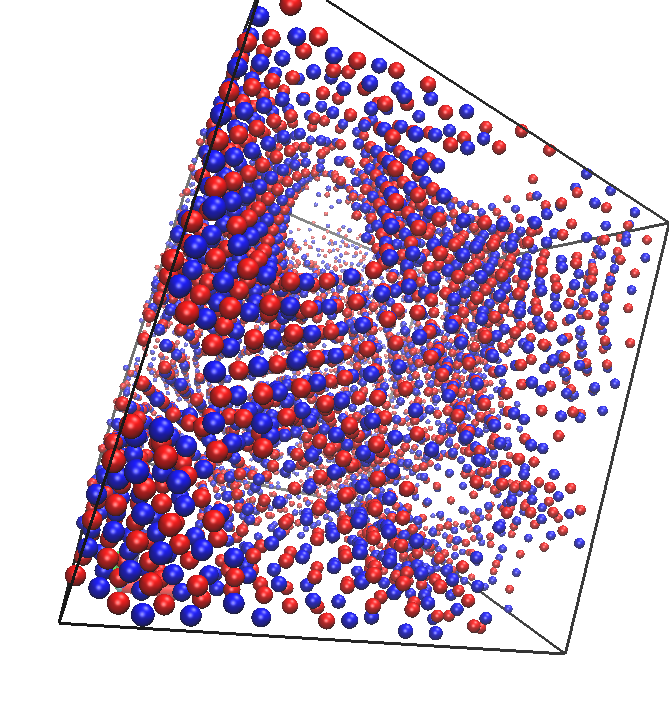
\includegraphics[width=\columnwidth]{coulomb/cou10-d0-08.png}
  \caption{$\rho=0.08\,\text{fm}^{-3}$, $\lambda=10\,\text{fm}$}
\end{subfigure}
\begin{subfigure}[h!]{0.5\columnwidth}
  \centering
  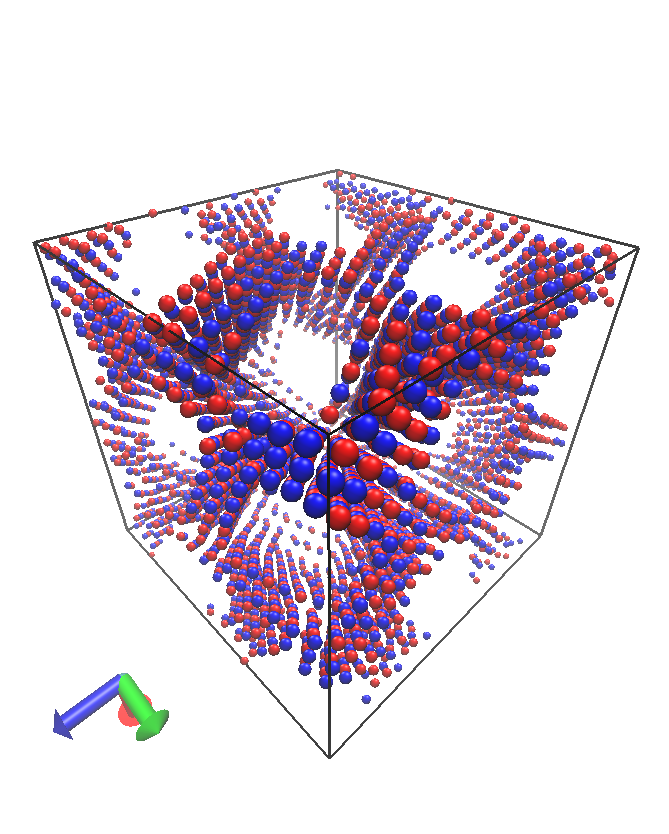
\includegraphics[width=\columnwidth]{coulomb/cou20-d0-08.png}
  \caption{$\rho=0.08\,\text{fm}^{-3}$, $\lambda=20\,\text{fm}$}
\end{subfigure}
\caption{Diferencia entre pasta con y sin interacción de Coulomb.
  Podemos ver que la interaccióñ de Coulomb separa la pasta, conviritendo una estructura por celda en múltiples estructuras por celda.}
\label{fig:w-wo-coulomb}
\end{figure}

Para comprender mejor cómo el estado de equilibrio a bajas temperturas varía a través del régimen de transición desde la inexistencia de Coulomb hacia un apantallamiento de $\lambda=20\,\text{fm}$, mostramos en la figura~\ref{fig:w-wo-coulomb} representaciones visuales de los resultados obtenidos para un conjunto de densidades elegidos, con $\lambda=0$, $\lambda=10\,\text{fm}$ y $\lambda=20\,\text{fm}$.
Vemos que obtenemos estructuras exóticas para $\lambda=10\,\text{fm}$ en los tres casos, que son variaciones de la estructura típica de la pasta que pueden deberse al complicado paisaje de energías para estos valores de $\lambda$.

\begin{figure}[h!]  %figure 5 \centering
\centering
\begin{subfigure}[h!]{0.4\columnwidth}
  \centering
  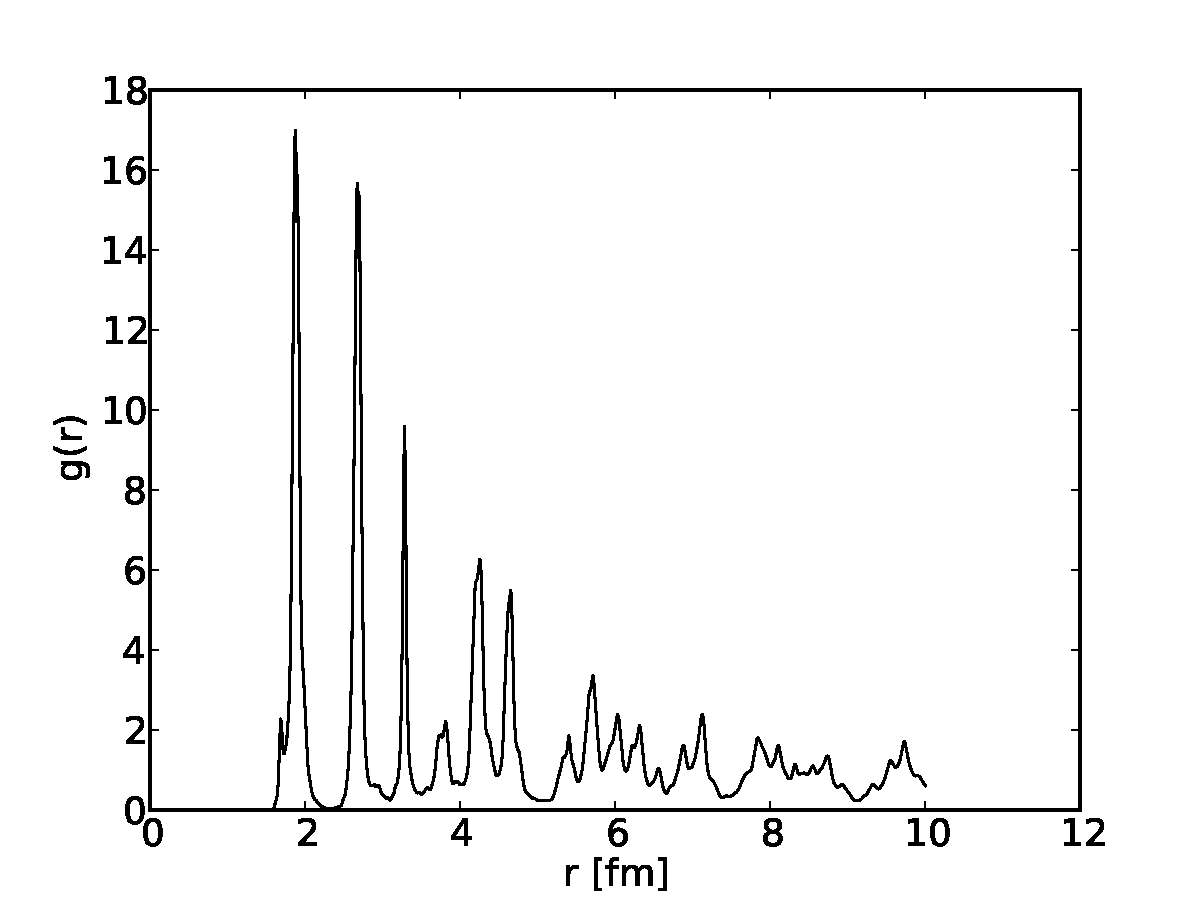
\includegraphics[width=\columnwidth]{coulomb/gofr-mult.pdf}
  \caption{Múltiples lasagnas}
\end{subfigure}
\begin{subfigure}[h!]{0.4\columnwidth}
  \centering
  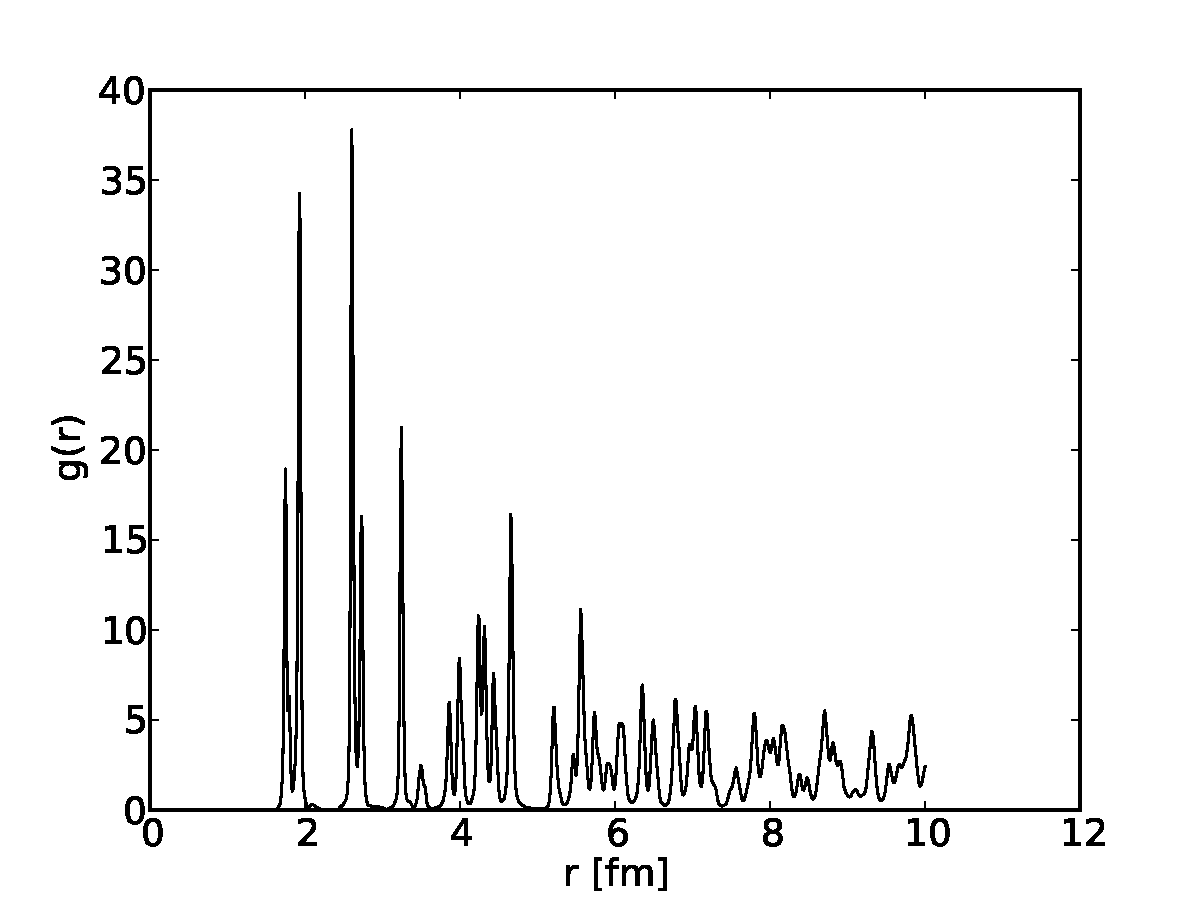
\includegraphics[width=\columnwidth]{coulomb/gofr-sing.pdf}
  \caption{Una lasagna}
\end{subfigure}
\caption{Ejemplos de la función distribución de pares para $\rho=0.05\,\text{fm}^{-3}$ y dos longitudes de apantallamiento:
  $\lambda=20\,\text{fm}$ y $\lambda=0\,\text{fm}$.
  Notar la diferencia en escalas en el eje $y$ para los dos gráficos.}
\label{fig:gofr}
\end{figure}

Como ejemplo, mostramos la función distribución de pares, $g(r)$, para $\rho=0.05\,\text{fm}^{-3}$ en la figura~\ref{fig:gofr}.
Aquí vemos que los primeros picos de la distribución se mantienen en las mismas distancias de $r=1.7\,\text{fm}, 1.9\,\text{fm}$ para ambas configuraciones.
Esto muestra que la estructura de rango corto está gobernada por el potencial nuclear incluso a $\lambda=20\,\text{fm}$, evidente simplemente al comparar los órdenes de magnitud de $V_{n-n}$ y $V_{\text{Coulomb}}$ para esos rangos.

Para la densidad $\rho=0.005\,\text{fm}^{-3}$, para longitudes de apantallamiento $\lambda<10\,\text{fm}$, hay un solo \emph{gnocchi}.
Sin embargo, cuando aumentamos de $\lambda=15\,\text{fm}$ a $\lambda=20\,\text{fm}$ para $\rho=0.005\,\text{fm}^{-3}$, aunque cualitativamente vemos el mismo comportamiento (ambos muestran \emph{gnocchi}), el tamaño promedio de los fragmentos es diferente para estos dos valores, de ahí la diferencia observada en las funcionales de Minkowski.
Para estudiar este resultado, graficamos el tamaño de los \emph{gnocchi} como función de $\lambda$ en la figura~\ref{fig:gnocchi_mass}.
Vemos que, cuanod tenemos en cuenta la varianza en la distribución de masa, se mantiene estable para $\lambda\geq20\,\text{fm}$.
El error relativo promedio del gráfico es $e\approx8\%$.

\begin{figure}[h] %figure 3
\centering
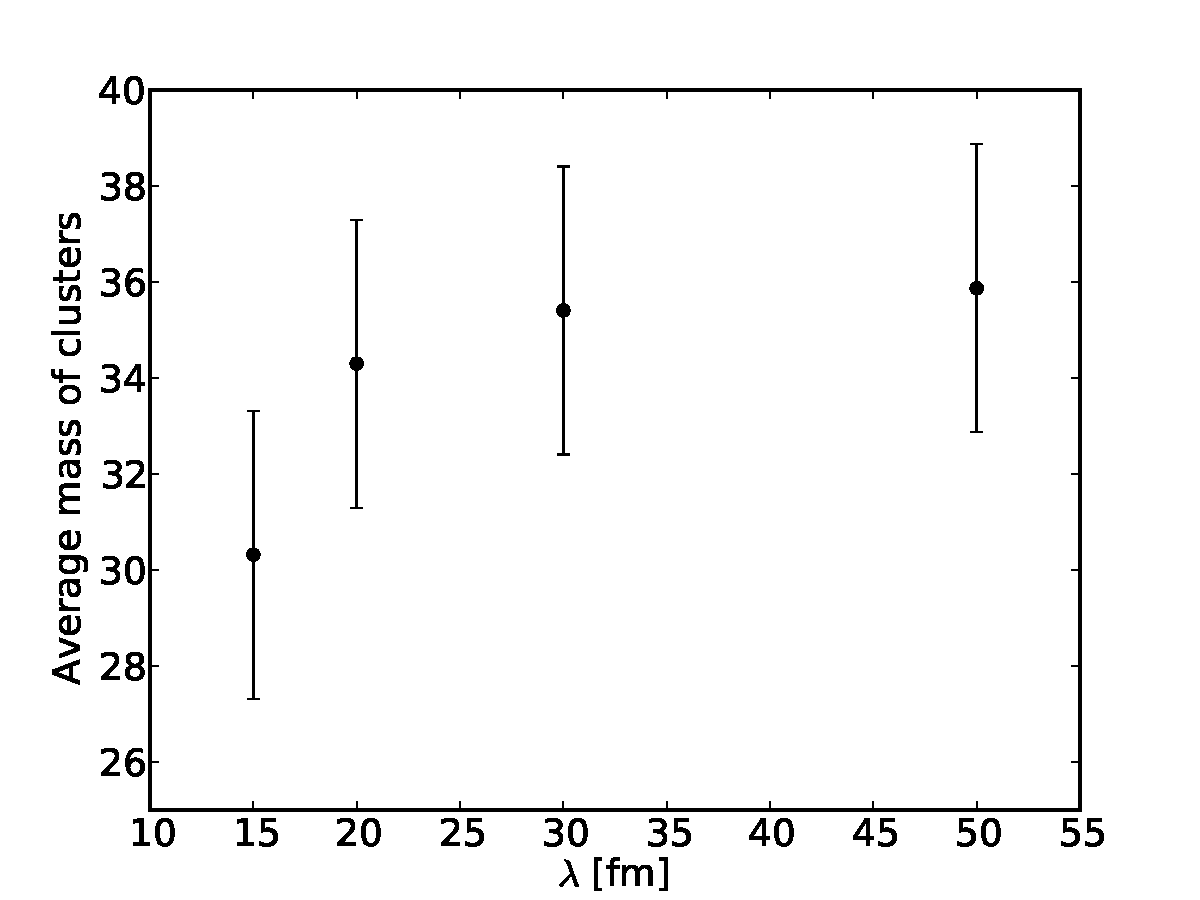
\includegraphics[width=\columnwidth]{coulomb/gnocchi_mass}
\caption{Tamaño promedio de los \emph{gnocchi} dependiendo de la longitud de apantallamiento.}
\label{fig:gnocchi_mass}
\end{figure}

Podemos ver que aunque odas las estructuras sin Coulombo son alguna de las pastas conocidas, una vez que agregamos la interacción de Coulomb (haciendo $\lambda\neq0$), la \emph{pseudo-pasta} original de $\lambda=0$ se separa: de una estrucutra por celda a múltiples estructuras por celda.
Para valores intermedios a bajos de $\lambda < 20\,\text{fm}$, el efecto de las condiciones periódicas de contorno es todavía observable para algunas densidadees y pueden aparece estructuras exóticas que no forman parte de las pastas usuales.

\section{The Transition Regime} \label{transition}

Vamos a estudiar ahora las estrucutras halladas en el régimen de transición.

Tomemos, por ejemplo, la densidad más baja ($\rho=0.005\,\text{fm}^{-3}$).
Como podemos ver de la figura~\ref{fig:gnocchi}, para $\lambda=0$ sólo se forma una gota, como era de esperar.
Para $\lambda=10\,\text{fm}$ aparecen muchos \emph{gnocchi}, pero algunos de ellos se adhieren a sus vecinos, formando estructuras proladas de diferentes tamaños.
A pesar de que la interacción de Coulomb es ahora suficientemente grande como para partir la estructura monolítica hallada con $\lambda=0$ en varias, las gotas resultantes no son los usuales \emph{gnocchi} que se ordenan en una red regular, como sí lo son las halladas para $\lambda=20\,\text{fm}$.

\begin{figure}[h!]  \centering
  \begin{subfigure}[h!]{0.25\columnwidth}
    \centering
    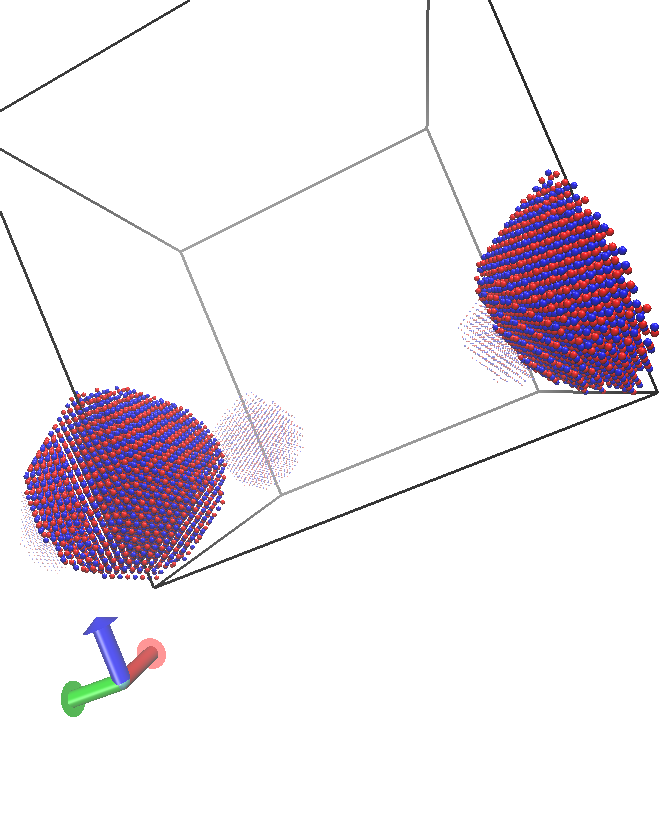
\includegraphics[width=\columnwidth]{coulomb/cou0-d0-005.png}
    \caption{$\lambda=0\,\text{fm}$}
  \end{subfigure}
  \begin{subfigure}[h!]{0.25\columnwidth}
    \centering
    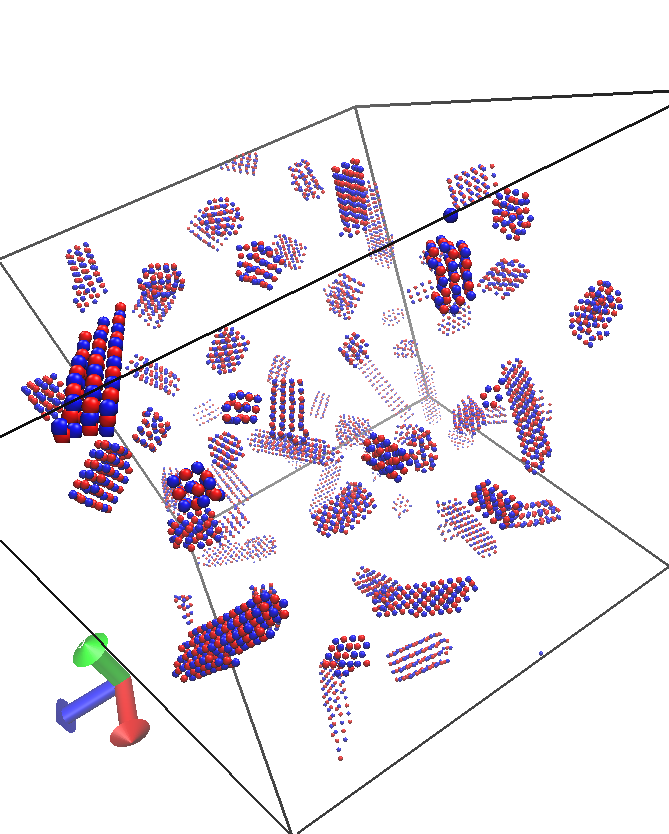
\includegraphics[width=\columnwidth]{coulomb/cou10-d0-005.png}
    \caption{$\lambda=10\,\text{fm}$}
  \end{subfigure}
  \begin{subfigure}[h!]{0.25\columnwidth}
    \centering
    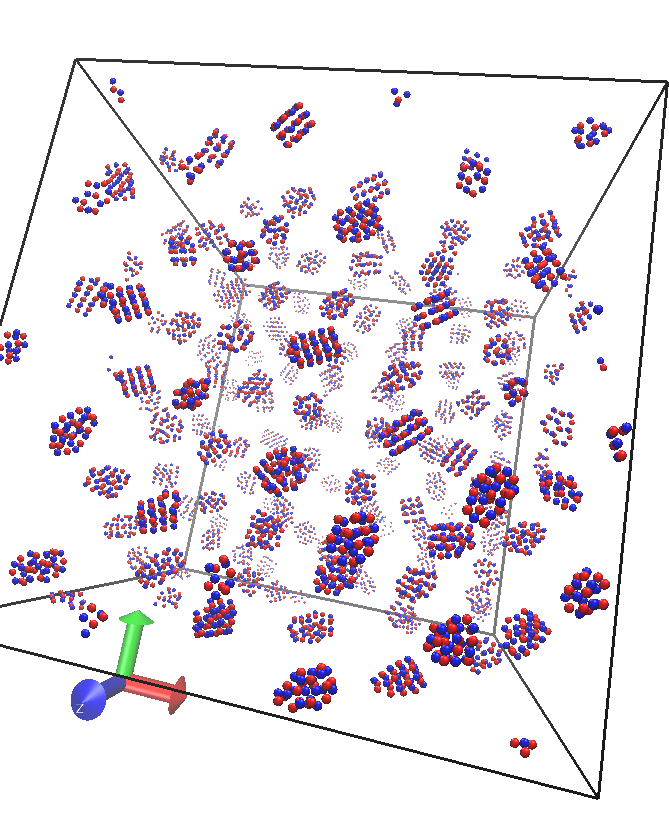
\includegraphics[width=\columnwidth]{coulomb/cou20-d0-005.png}
    \caption{$\lambda=20\,\text{fm}$}
  \end{subfigure}
  \caption{Diferentes estructuras halladas al variar la longitud de apantallamiento $\lambda$, para $\rho=0.005\text{fm}^{-3}$.
    En el régimen de transición hallamos, para $\lambda=10\,\text{fm}$, que la estructura se parte en varios fragmentos prolados, parecidos a \emph{spaghetti} cortados.}
  \label{fig:gnocchi}
\end{figure}


\section{Conclusiones}\label{concluding}

Estudiamos el efecto de la longitud de apantallamiento de la interacción de Coulomb en las simulaciones de materia de estrellas de neutrones a densidad comparables a las de la corteza de las estrellas de neutrones.
A lo largo de la literatura podemos encontrar que el valor de la longitud de apantallamiento en la aproximación de Thomas-Fermi es $\lambda\approx100\,\text{fm}$.
Para simulaciones basadas en partículas, debido a las limitaciones computacionales, este valor fue histórica y aribtrariamente reducido a $\lambda\approx10\,\text{fm}$, esperando mantener la fenomenología básica cuando se estudiaban sistemas pequeños.
Encontramos, sin embargo, que existe una longitud de apantallamiento crítica $\lambda_c$ a la cual la estructura del estado fundamental cambia drásticamente.
Para el potencial de Pandharipande en su paramatrización Medium, yace entre $10\,\text{fm}$ and $15\,\text{fm}$ (dependiendo de la densidad).
Para $\lambda<\lambda_c$, la interacción de Coulomb apenas actúa y las estructuras no homogéneas que emergen de las simulaciones se deben a efectos de tamaño finito, como es evidente a partir de la presión negativa de estas estructuras y el hecho de que hay sólo una estructura por celda.
Para $\lambda>\lambda_c$ la presión se vuelve positiva y los sistemas presentan fluctuaciones de densidad a una escala menor que la de la celda, pero no con la forma de la pasta típica.
Este régimen de transición se caracteriza por grandes fluctuaciones en la superficie, ancho medio y característica de Euler $\chi$ de las estructuras.
Es recién para $\lambda=20\,\text{fm}$ que la morfología de las estructuras se estabiliza y deja de depender de $\lambda$.
Más aún, las estructuras en este régimen son las pastas usuales.

Debido a esto, creemos que se tiene que tomar extrema precaución cuando se elige un valor arbitrario de $\lambda$, ya que aunque algunos resultados a $\lambda=10\,\text{fm}$ pueden ser como la pasta sperada, los resultados obtenidos para esa elección particular de $\lambda$ pueden ser cualitativamente diferente de aquellos en la correcta aproximación de Thomas-Fermi.
En conclusión, encontramos que la elección de un buen valor para $\lambda$ que vuelve al sistema computable computacionalmente y puede adecuadamente recuperar la física de la aproximación de Thomas-Fremi no es una tarea trivial, y se necesita un estudio riguroso antes de escogerlo.
Un buen valor de $\lambda$ debe cumplir $\lambda>\lambda_c$, que depende del modelo utilizado para la interacción nuclear.



\chapter[Transiciones de fase]{Transiciones de fase}
\label{ch:transicion}
En este capítulo tratamos las distintas escalas de longitud que aparecen en la dinámica de los nucleones en condiciones acordes a las de la corteza de las estrellas de neutrones, estudiando materia simétrica en isospín (igual cantidad de protones y neutrones) a densidades menores a la de saturación para 5000 partículas.
Variando la temperatura encontramos una transición de fase sólido-líquido que se puede caracterizar también como una transición topológica.
Para temperaturas más altas que la de la transición de fase estudiamos la opacidad de los neutrinos y encontramos que en la fase líquida el \emph{scattering} de los neutrinos de bajo momento se mantiene elevado, incluso con morfologías que son significativamente diferentes a las de la pasta nuclear tradicional.


\section{Introducción}

En este capítulo utilizamos distintas herramientas topológicas y termodinámicas para caracterizar la materia de estrellas de neutrones simétrica, en función de caracterizar la fase en la que se encuentra.

\subsection{Herramientas Topológicas}

Una de las herramientas topológicas que utilizamos son los funcionales de Minkowski.
Las medidas topológicas de un cuerpo convexo $K \in \mathcal{R}$ se definen como funcionales $\varphi: \mathcal{R} \rightarrow \mathbb{R}$ que satisfacen tres propiedades:

\begin{description}
  \item{Invariancia de movimiento:} $\varphi(K) = \varphi(g(K))$, donde $g(K)$ implica cualquier tipo de traslación y rotación del cuerpo $K$.
  \item{Aditividad:} $\varphi(K_1 \cup K_2) = \varphi(K_1) + \varphi(K_2) - \varphi(K_1 \cap K_2)$.
  \item{Continuidad:} $\lim_{n\rightarrow\infty}\varphi(K_n) = \varphi(K)$ si $\lim_{n\rightarrow\infty}K_n = K$, donde ${K_n}$ es un conjunto de cuerpos convexos.
\end{description}

El teorema de Hadwiger dice que para un sistema de dimensión $d$ hay sólo $d+1$ funcionales independientes que satisfacen las propiedades mencionadas: las funcionales de Minkowski. En el espacio tridimensional, las funcionales de Minkowski están asociadas al volumen, el área, la curvatura media y el número de Euler. A pesar de que no necesariamente las estructuras obtenidas en este trabajo sean convexas (es decir, las funcionales de Minkowski no las definen unívocamente), utilizamos estas medidas para caracterizarlas. En el apéndice~\ref{ap:minkowski} se puede observar detalladamente el cálculo de estas magnitudes.

Además de las funcionales de Minkowski, utilizamos la función distribución de pares, usualmente denominada $g(r)$, que se define a partir de un histograma de todas las distancias entre pares de partículas.
Este histograma luego se normaliza con respecto al del gas ideal, donde las distancias están completamente descorrelacionadas.
Para tres dimensiones, esta normalización es la densidad multiplicada por el volumen de un cascarón esférico.

\subsection{Herramientas Termodinámicas}

Además de las clásicas señales termodinámicas para las transiciones de fase de primer o segundo orden, utilizamos el coeficiente de Lindemann.
El coeficiente de Lindemann se basa en las fluctuaciones de las partículas alrededor del punto de equilibrio, y es utilizado especialmente para estudiar transiciones de tipo sólido-líquido en sistemas infinitos, como los cristales.
Se define a partir de la desviación estándar de las posiciones de las partículas, $\Delta
r_i^2$:

\begin{equation*}
\Delta_L = \frac{\sqrt{\sum_i\langle\Delta r_i^2/N\rangle}}{a}
\end{equation*}
donde $a$ es la constante de red del cristal y $N$ el número total de partículas.
En nuestro caso, escogemos $a=(V/N)^{1/3}$, la longitud característica del sistema.


\section{Transición de fase}\label{phase_transition}
\subsection{Transición de fase termodinámica}

La figura~\ref{fig:energy} presenta la energía como función de la temperatura (curva calórica) para distintas densidades.
Cada una de estas densidades exhibe una discontinuidad en la energía para ciertas temperaturas, una señal de una transición de fase de primer orden.
Esta transición puede ser confirmada y caracterizada como de sólido-líquido observando el coeficiente de Lindemann. Por ejemplo, mostramos el coeficiente de Lindemann junto a la energía para $\rho=0.05\,\text{fm}^{-3}$ en la figura~\ref{fig:lind-energ}.
Esta figura muestra que las discontinuidades en las energía y en el coeficiente de Lindemann están a la misma temperatura.
Éstas dos son características de la transición de fase sólido-líquido.

\begin{figure}[h!]  \centering
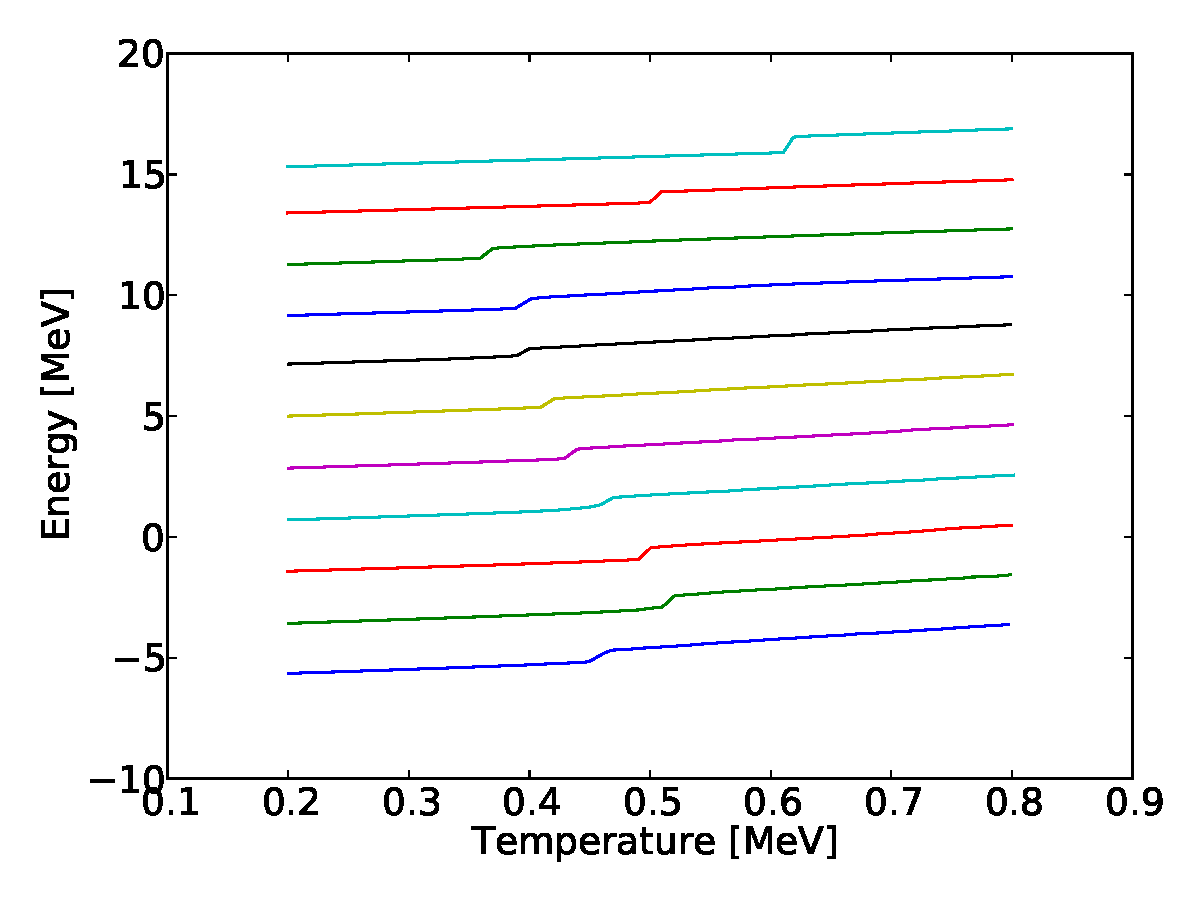
\includegraphics[width=0.7\columnwidth]{transicion/energy.pdf}
\caption{Energía como función de la temperatura para distintas densidades.
  Observamos una discontinuidad en el rango desde $T_l=0.35\,\text{MeV}$ a $T_h=0.65\,\text{MeV}$, dependiendo de la densidad.
  Esto es una señal de una transición de fase.
  En la figura, las densidades van de $\rho=0.03\,\text{fm}^{-3}$ a $\rho=0.13\,\text{fm}^{-3}$, incrementando $\Delta\rho=0.01\,\text{fm}^{-3}$ hacia arriba.}
\label{fig:energy}
\end{figure}

\begin{figure}[h!]  \centering
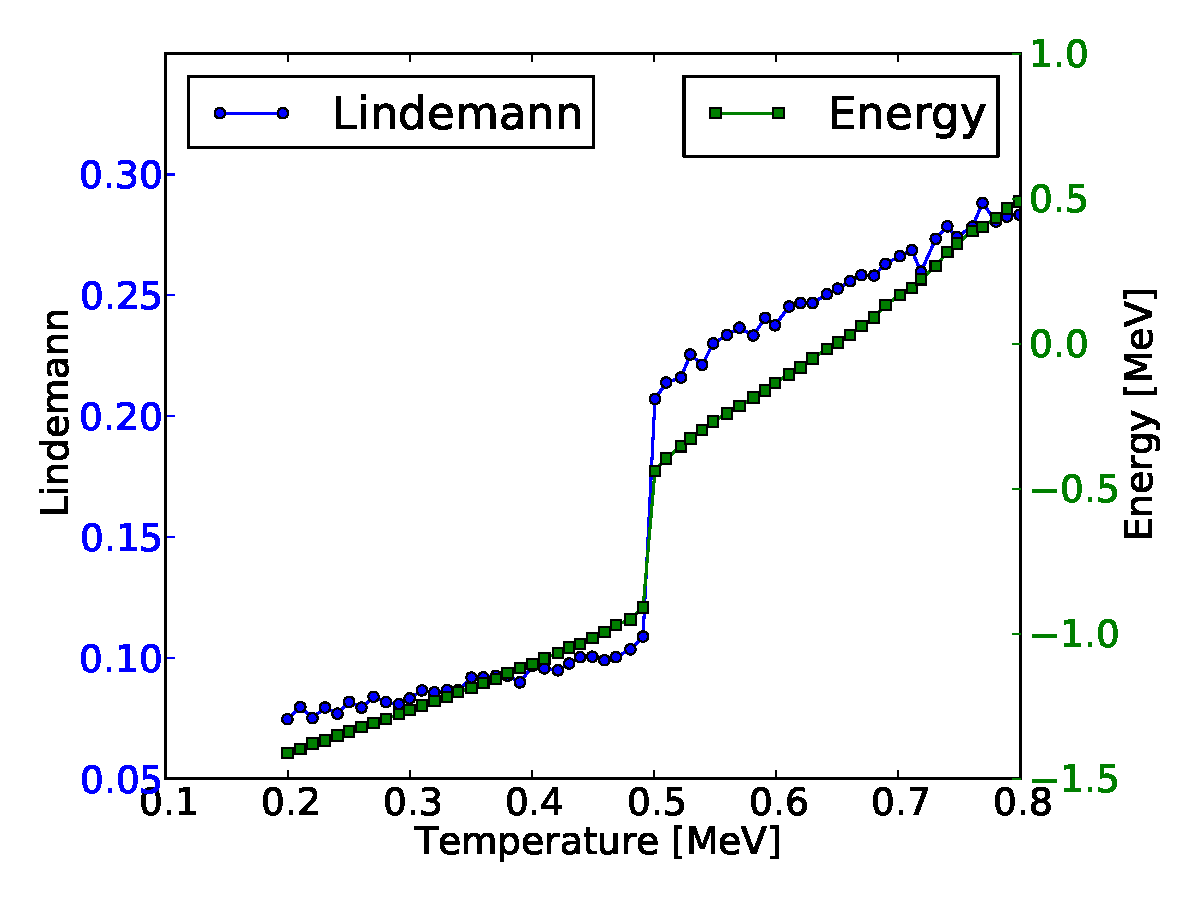
\includegraphics[width=0.7\columnwidth]{transicion/lind-energ.pdf}
\caption{Coeficiente de Lindemann y energía como función de la temperatura para una densidad, $\rho=0.05\,\text{fm}^{-3}$.
  El cambio abrupto en su valor es una señal de una transición de fase sólido-líquido.
  Podemos ver que ambas discontinuidades están a la misma temperatura.}
\label{fig:lind-energ}
\end{figure}

En la figura~\ref{fig:rdf} mostramos la función de distribución de pares para tres densidades distintas: $\rho=0.03\,\text{fm}^{-3}$ (\emph{spaghetti}), $\rho=0.05\,\text{fm}^{-3}$ (\emph{lasagna}) y $\rho=0.08\,\text{fm}^{-3}$ (túneles), inmediatamente sobre y bajo la temperatura de transición, así como una foto del sistema en la fase de temperatura alta.
Como los primeros picos (correspondientes a los primeros vecinos) están en la misma posición más allá de la temperatura, concluimos que el orden corto está presente tanto sobre como bajo la transición.
Sin embargo los los picos de los terceros vecinos, distintivos de las fases sólidas, desaparecen a medida que la temperatura aumenta más allá de la transición.
El orden de muy largo rango también sobrevive a la transición, como discutimos más adelante en la sección~\ref{very_long}

\begin{figure}
  \centering
  \begin{subfigure}[h!]{0.4\columnwidth}
    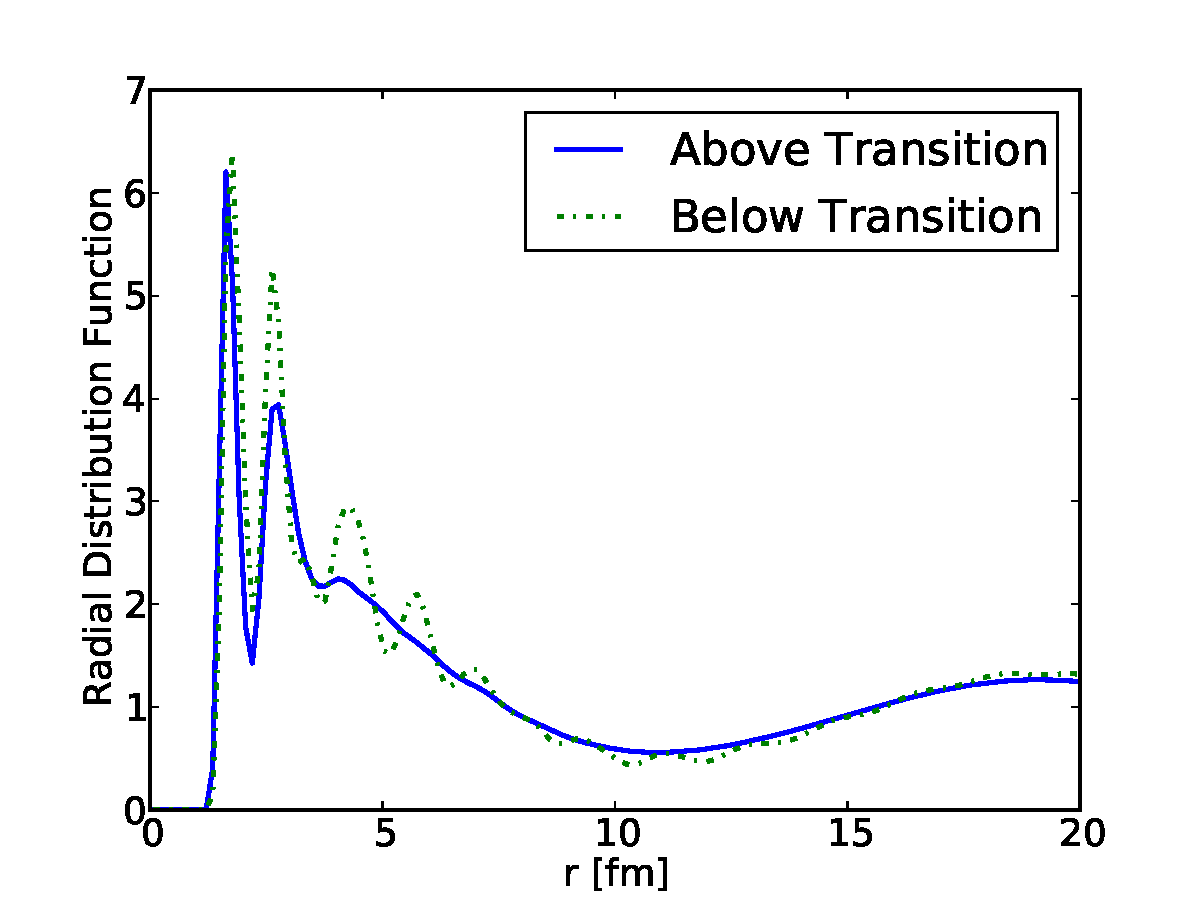
\includegraphics[width=\columnwidth]{transicion/rdf_0-03.pdf}
    \caption{Función de distribución de pares para $\rho=0.03\,\text{fm}^{-3}$}
  \end{subfigure}
  \begin{subfigure}[h!]{0.3\columnwidth}
    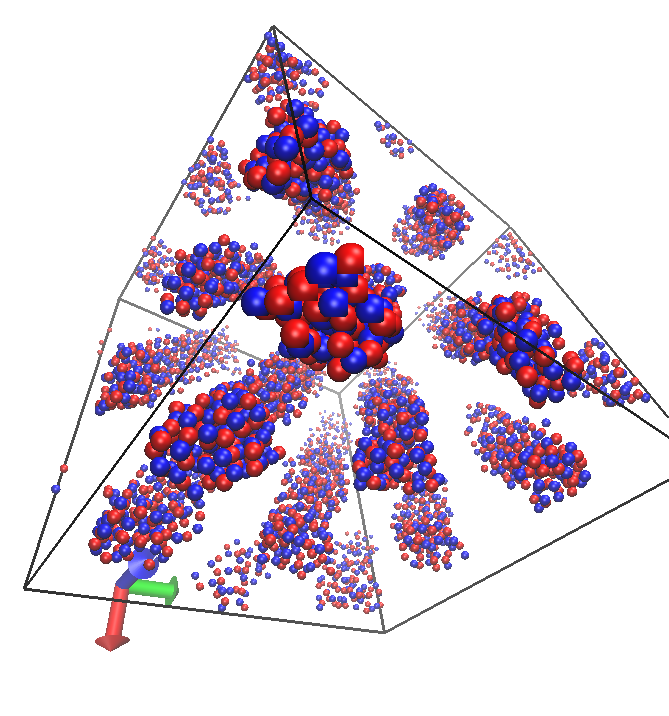
\includegraphics[width=\columnwidth]{transicion/morph_0-03_0-47.png}
    \caption{Foto del sistema en la fase líquida para $\rho=0.03\,\text{fm}^{-3}$}
  \end{subfigure}
  \begin{subfigure}[h!]{0.4\columnwidth}
    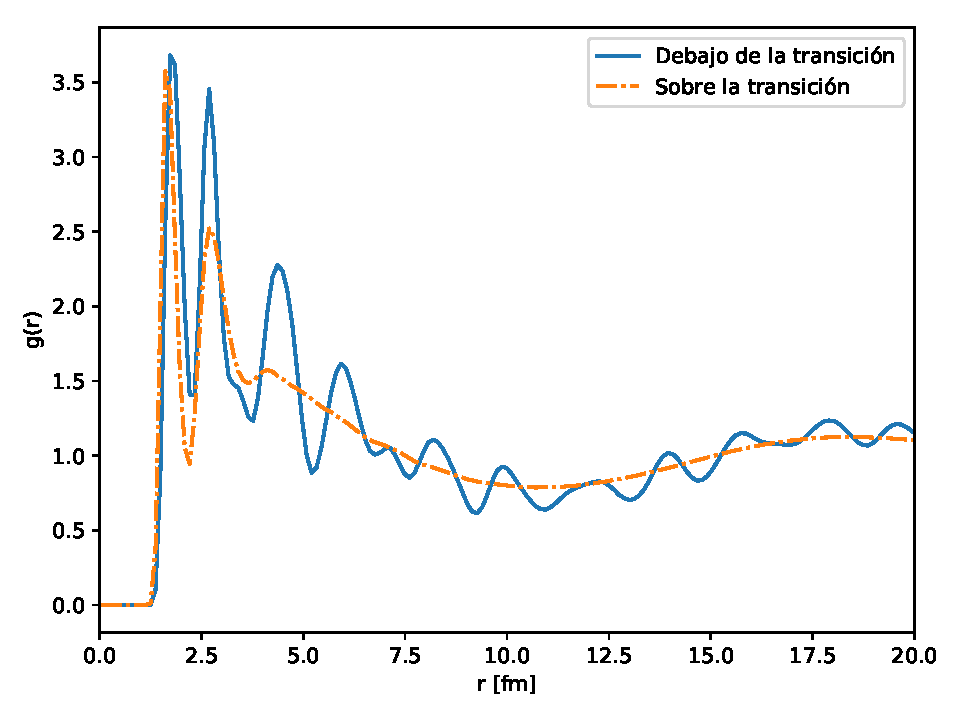
\includegraphics[width=\columnwidth]{transicion/rdf_0-05.pdf}
    \caption{Función de distribución de pares para $\rho=0.05\,\text{fm}^{-3}$}
  \end{subfigure}
  \begin{subfigure}[h!]{0.3\columnwidth}
    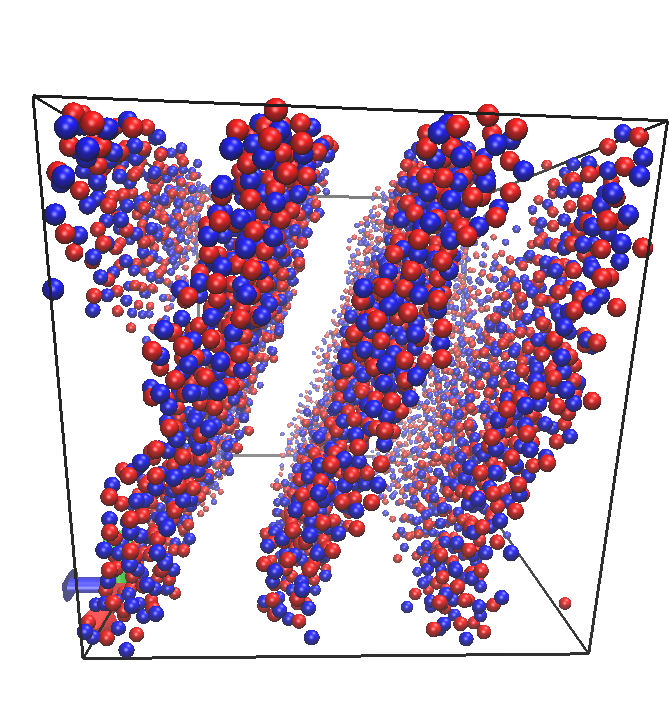
\includegraphics[width=\columnwidth]{transicion/morph_0-05_0-50.png}
    \caption{Foto del sistema en la fase líquida para $\rho=0.05\,\text{fm}^{-3}$}
  \end{subfigure}
  \begin{subfigure}[h!]{0.4\columnwidth}
    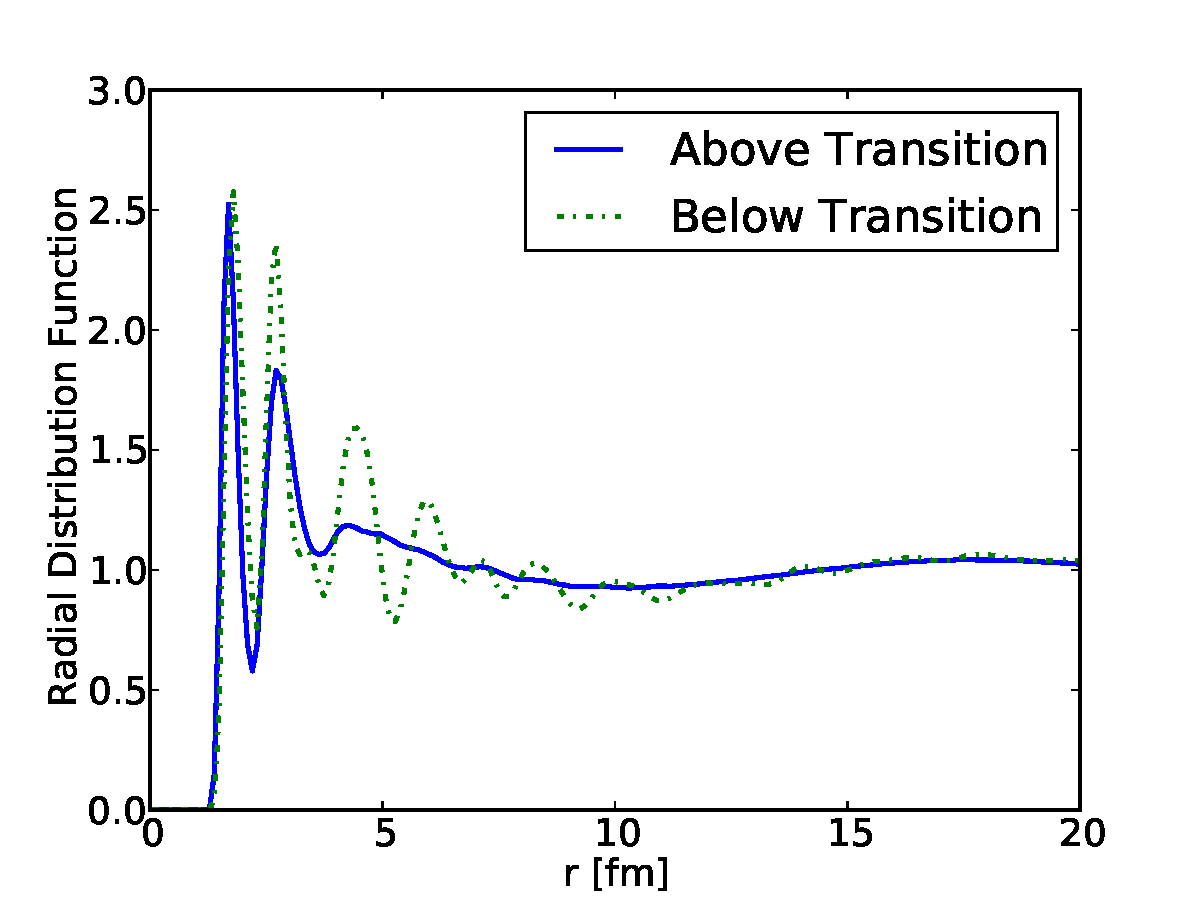
\includegraphics[width=\columnwidth]{transicion/rdf_0-08.pdf}
    \caption{Función de distribución de pares para $\rho=0.08\,\text{fm}^{-3}$}
  \end{subfigure}
  \begin{subfigure}[h!]{0.3\columnwidth}
    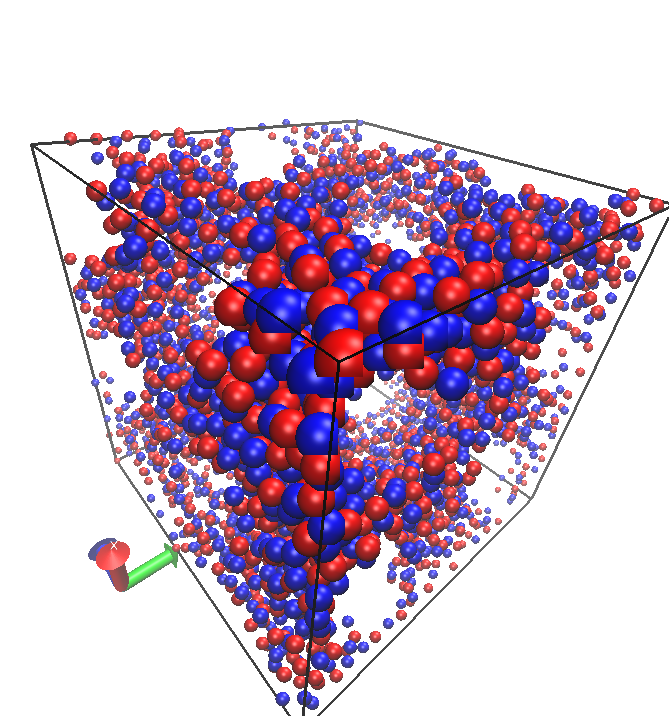
\includegraphics[width=\columnwidth]{transicion/morph_0-08_0-42.png}
    \caption{Foto del sistema en la fase líquida para $\rho=0.08\,\text{fm}^{-3}$}
  \end{subfigure}
  \caption{Función de distribución de pares para distintas densidades, tanto debajo como sobre la temperatura de transición, y foros del sistema en la fase líquida.
Aunque los primeros picos de la distribución están en las mismas posiciones para ambas temperaturas, los picos siguientes, que exhiben un orden de rango largo típico de los sólidos, sólo están presentes por debajo de la temperatura de transición.}
  \label{fig:rdf}
\end{figure}

\subsection{Transición de fase topológica}
Cuando observamos los funcionales de Minkowski, particularmente la característica de Euler y el ancho medio, observamos que también hay una temperatura ``crítica'' en la cual ambas magnitudes exhiben una transición abrupta.
Mostramos, como un ejemplo, estas magnitudes como función de la temperatura para la densidad
$\rho=0.05\,\text{fm}^{-3}$ en la figura~\ref{fig:euler-curv}.
Como esta transición está señalada por los observables topológicos, concluimos que es una transición también topológica, que se forma porque las partículas comienzan a moverse dentro de la estructura, dejando agujeros en su interior.

\begin{figure}%[H]
  \centering 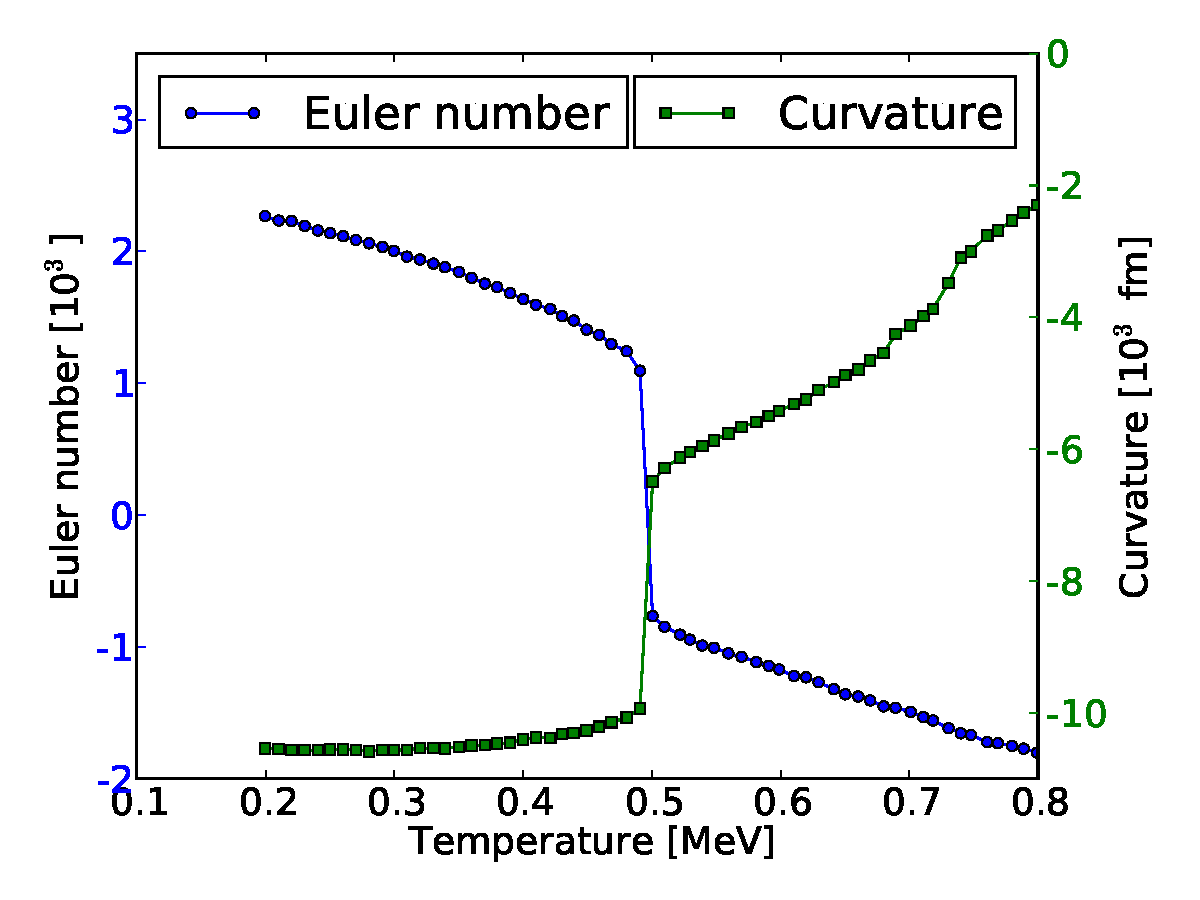
\includegraphics[width=0.7\columnwidth]{transicion/euler-curv.pdf}
  \caption{Número de Euler y ancho medio para $\rho=0.05\,\text{fm}^{-3}$.
    Observamos una transición abrupta para ambas funcionales de Minkowski.}
  \label{fig:euler-curv}
\end{figure}

Estas señales de una transición sólido-líquido (discontinuidad en la energía y en el coeficiente de Lindemann) y topológica (discontinuidad en las funcionales de Minkowski) se producen a la misma temperatura de transición, como se puede observar en el diagrama de fases de la figura~\ref{fig:critical_temperature}.
Esto significa que, a medida que el sistema es enfriado a un volumen fijo, sufre una transición termodinámica y topológica a la misma temperatura.

\begin{figure}
  \centering
  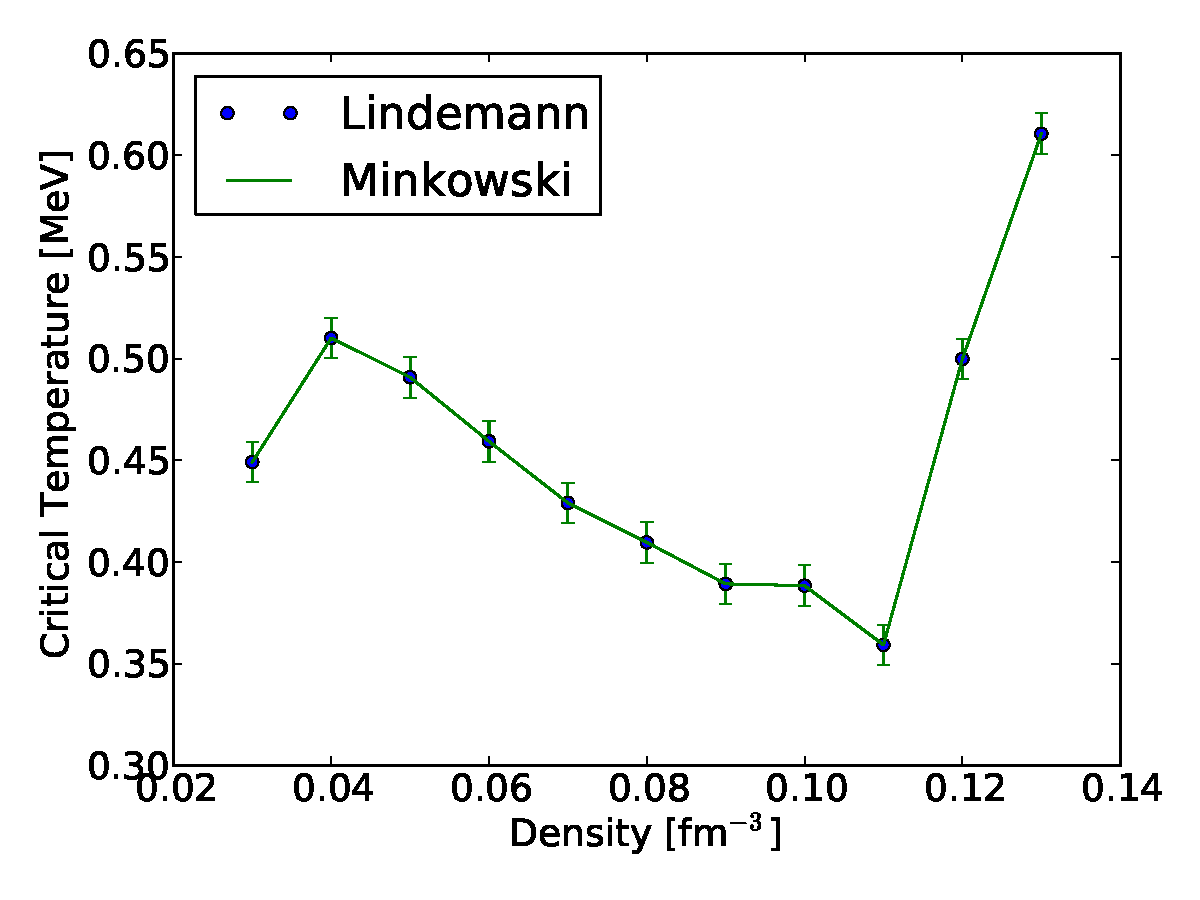
\includegraphics[width=0.6\columnwidth]{transicion/critical_temperature.pdf}
  \caption{Temperatura crítica como función de la densidad.
    Observamos la superposición entre la temperatura crítica de las funcionales de Minkowski y el coeficiente de Lindemann.}
  \label{fig:critical_temperature}
\end{figure}


\section{Comportamiento de muy largo rango}\label{very_long}
Además de que desaparece el orden de corto largo característico de los sólidos, otra característica es evidente de la figura~\ref{fig:rdf}.
Una modulación de muy largo en la función de distribución de pares sobrevive a través de la transición de sólido-líquido.
Este orden de muy largo rango es característico de las fases de la pasta.
En la figura~\ref{fig:morph} mostramos la configuración espacial para $\rho=0.05\,\text{fm}^{-3}$, para temperaturas tanto sobre como debajo de la temperatura de transición.
En ella vemos que no sólo la fase sólida tiene la forma usual de la plasta, sino que además la fase líquida la preserva.
Debajo de a transición, tenemos ``pasta congelada''.
Justo por sobre ella, los nucleones pueden fluir, pero confinados a cierta pasta o estructura tipo-pasta, como vemos en las siguientes secciones.

\begin{figure*}[floatfix]%[H]
  \centering
  \begin{subfigure}[h!]{0.48\columnwidth}
    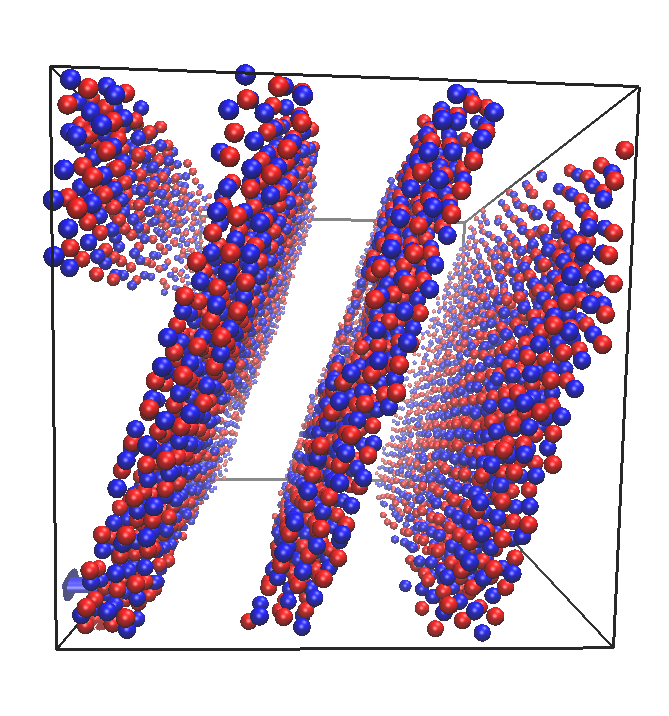
\includegraphics[width=\columnwidth]{transicion/morph_0-05_0-48.png}
    \caption*{Debajo de la transición.}
  \end{subfigure}
  \begin{subfigure}[h!]{0.48\columnwidth}
    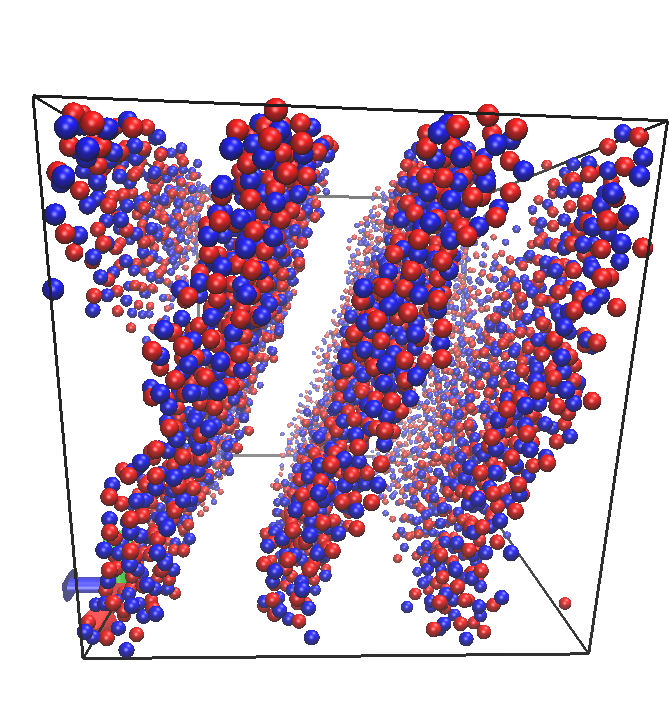
\includegraphics[width=\columnwidth]{transicion/morph_0-05_0-50.png}
    \caption*{Sobre la transición.}
  \end{subfigure}
  \caption{Distribución espacial para $\rho=0.05\,\text{fm}^{-3}$, tanto sobre como debajo de la temperatura de transición.
    Las estructuras son similares, pero mucho más desordenadas sobre la transición.}
  \label{fig:morph}
\end{figure*}

\section{Propiedades de transporte de neutrinos}
Este orden de muy largo rango, evidente de la figura~\ref{fig:rdf}, es responsable del pico a muy bajo momento $k$ (longitud de onda $\lambda\sim 10\,\text{fm}$) en el factor de estructura $S(k)$, proporcional a la probabilidad de scattering.
Con esto en mente, ahora nos enfocamos en el orden de muy largo rango para nuestras estructuras.

En la figura~\ref{fig:sk_peak_0-05} graficamos la altura del pico del factor de estructura para momentos bajos $S(k<0.5\,\text{fm}^{-1})$ ($\lambda\gtrsim13\,\text{fm}$) como función de la temperatura para $\rho=0.05\,\text{fm}^{-3}$.
La forma más intuitiva para leer esta figura es de derecha a izquierda (de temperaturas altas a bajas), reproduciendo el procedimiento de enfriado del sistema en nuestras simulaciones.
Cada línea corresponde a evoluciones con distintas condiciones iniciales, pero manteniendo el mismo protocolo de enfriamiento y los mismos criterios de estabilidad.

\begin{figure}
  \centering
  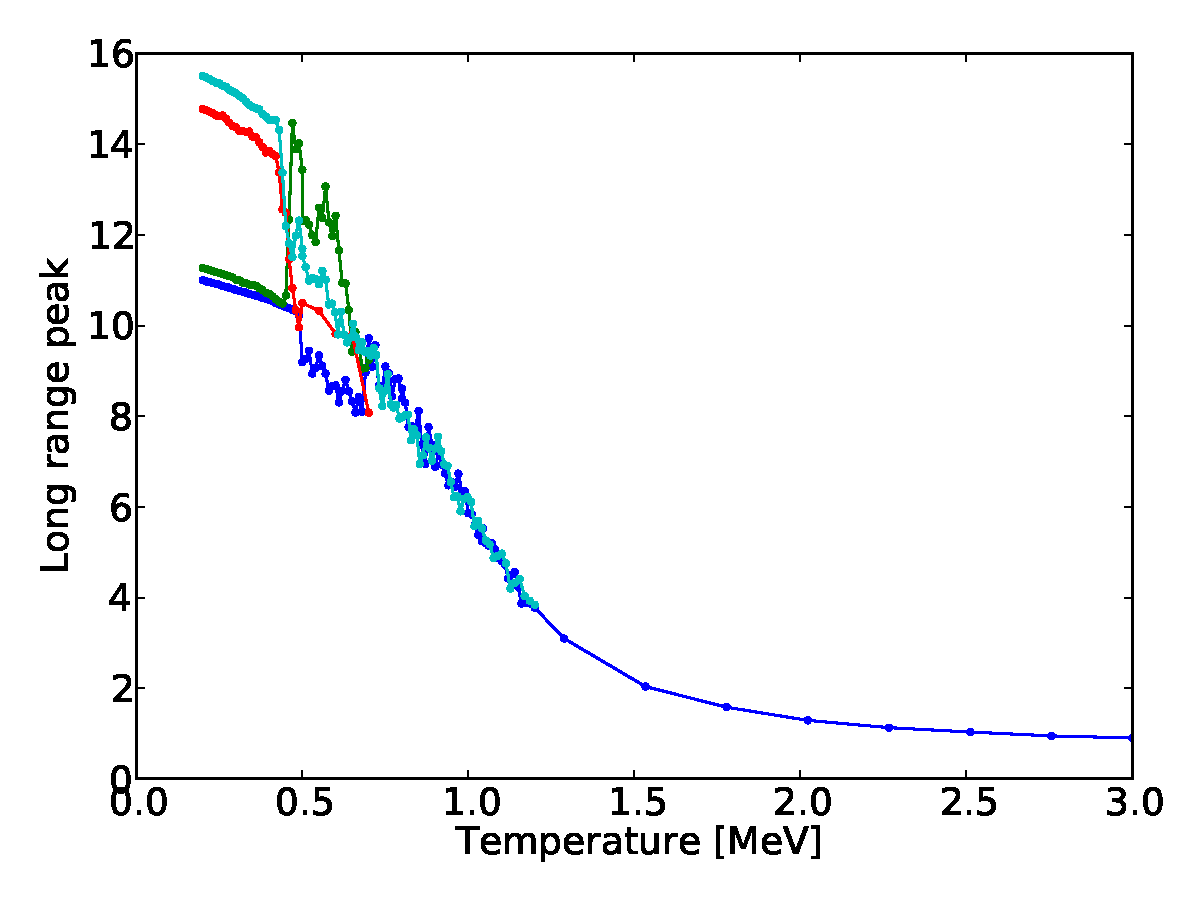
\includegraphics[width=0.7\columnwidth]{transicion/sk_peak_0-05.pdf}
  \caption{Pico de $S(k)$ para momentos bajos como función de la temperatura, para $\rho=0.05\,\text{fm}^{-3}$.
    Observamos dos comportamientos para $T<0.5\,\text{MeV}$ y $T>0.5\,\text{MeV}$.  }
  \label{fig:sk_peak_0-05}
\end{figure}

\begin{figure}
  \centering
  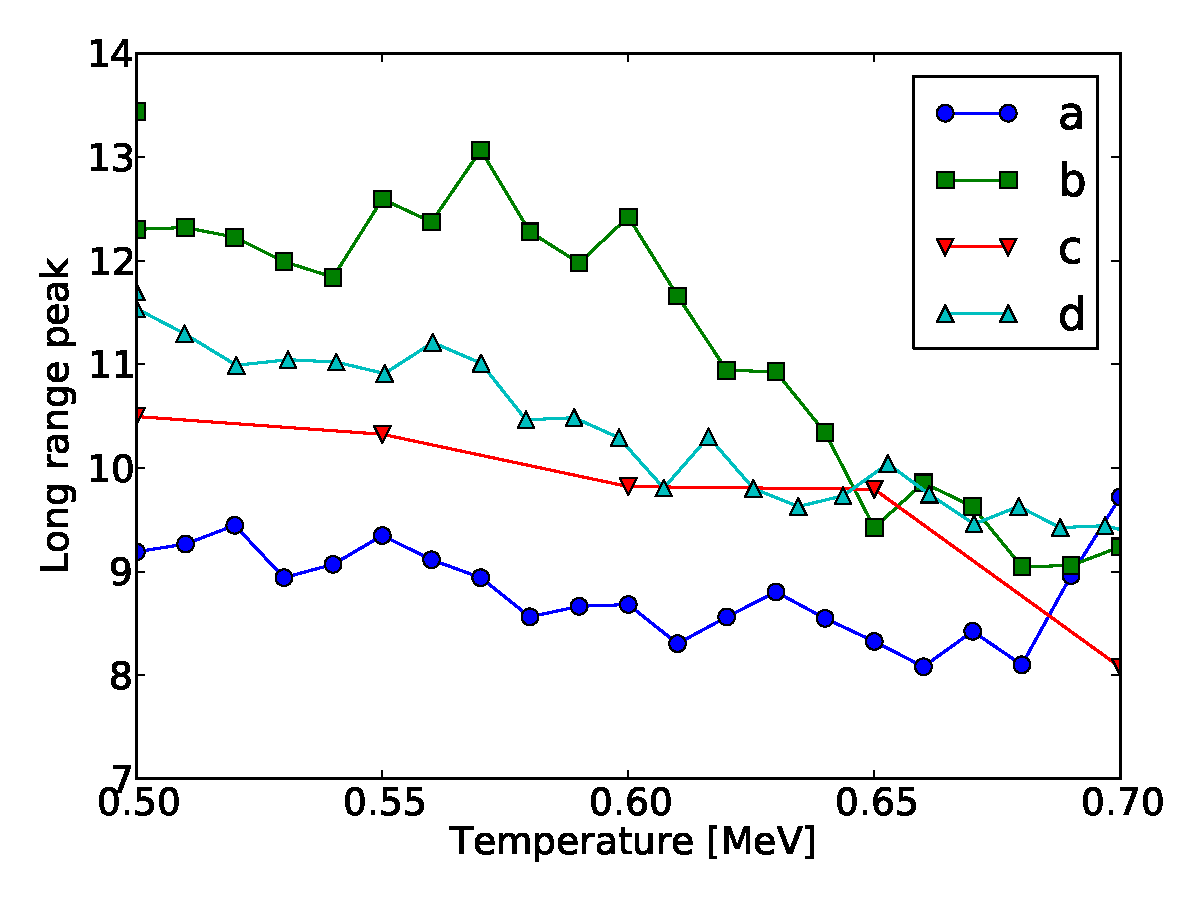
\includegraphics[width=0.7\columnwidth]{transicion/sk_peak_zoom.pdf}
  \caption{Pico de $S(k)$ para momentos bajos, en el rango de temperaturas entre $T=0.5\,\text{MeV}$ y $T=0.7\,\text{MeV}$.
    Observamos que distintas condiciones iniciales conducen a distintos picos de absorción para bajos momentos.}
  \label{fig:sk_peak_zoom}
\end{figure}

A temperaturas suficientemente altas ($T\sim 2\,\text{MeV}$) los nucleones están distribuidos de forma bastante homogénea, y no se evidencia ninguna estructura a partir de la $S(k)$: el ``pico'' desaparece, tendiendo a 1 (el valor para sistemas homogéneos).
A medida que la temperatura decrece aparece un pico en los momentos bajos.
La transición descripta en la sección \ref{phase_transition} se manifiesta en la figura~\ref{fig:sk_peak_0-05} a partir de la ausencia de fluctuaciones para temperaturas menores a la de transición $T \lesssim 0.5\,\text{MeV}$.
Incluso a temperaturas altas como
$T=1.0\,\text{MeV}$ aún hay un pico de absorción reconocible para momentos bajos (con altura claramente mayor a 1), pero no siempre se corresponde a la forma de una pasta usual (\emph{gnocchi}, \emph{spaghetti} o
\emph{lasagna}) en nuestras simulaciones.
A estas temperaturas, y para la mayoría de las densidades, la estructura del sistema es parecida a una ``esponja'' que tiene, de cualquier modo, inhomogeneidades lo suficientemente notables como para producir un pico reconocible en $S(k)$.

Es interesante notar que cuando el sistema llega a temperaturas de $T\sim 0.7\,\text{MeV}$ observamos que distintas ejecuciones de la simulación causan que el sistema ``colapse'' en distintas estructuras, además de la \emph{lasagna} usual.
Podemos observar en detalle la altura del pico de  $S(k)$ para esta región de temperaturas en la figura~\ref{fig:sk_peak_zoom} y las estructuras que corresponden a cada una de las simulaciones en la figura~\ref{fig:cool_morph} (ver epígrafe para detalles).

\begin{figure*}[floatfix]%[H]
  \centering
  \begin{subfigure}[h!]{0.35\columnwidth}
    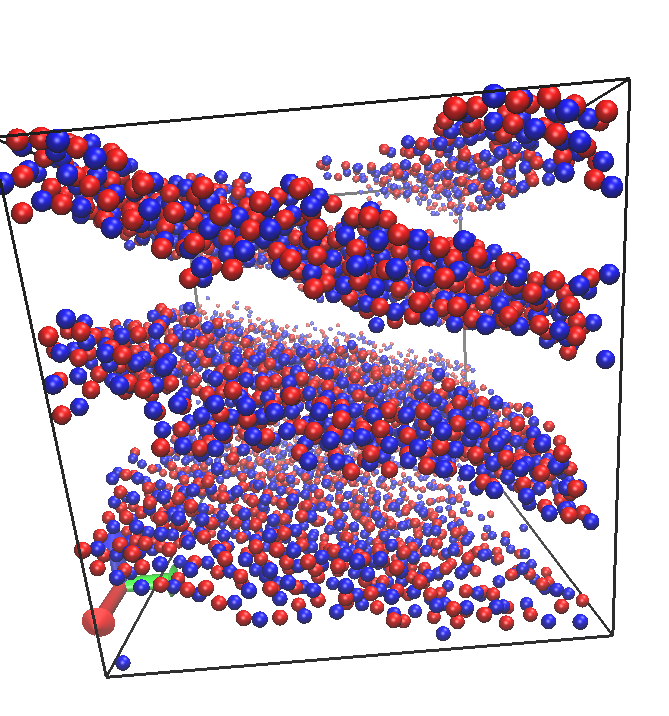
\includegraphics[width=\columnwidth]{transicion/morph_02-08-001.png}
    \caption{\emph{Lasagna} usual}
  \end{subfigure}
  \begin{subfigure}[h!]{0.35\columnwidth}
    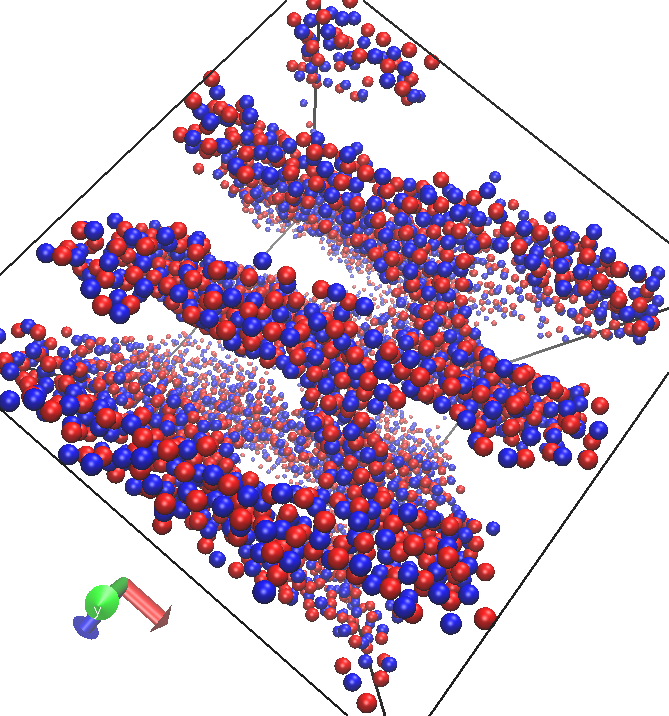
\includegraphics[width=\columnwidth]{transicion/morph_05-07-001.png}
    \caption{\emph{Lasagna} interconectada}
  \end{subfigure}
  \begin{subfigure}[h!]{0.35\columnwidth}
    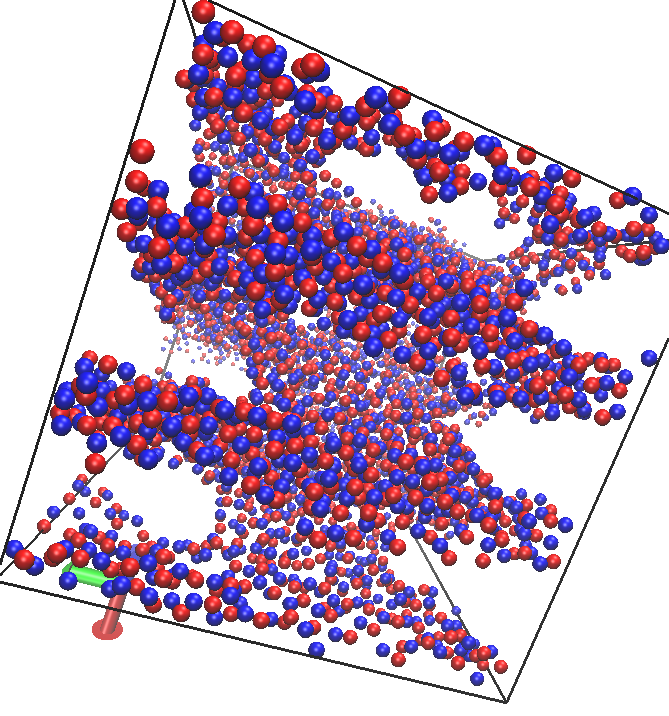
\includegraphics[width=\columnwidth]{transicion/morph_05-12-0013.png}
    \caption{\emph{Lasagna} interconectada}
  \end{subfigure}
  \begin{subfigure}[h!]{0.35\columnwidth}
    \includegraphics[width=\columnwidth]{transicion/morph_decorr.png}
    \caption{Pasta inusual}
  \end{subfigure}
  \caption{Estructuras del sistema para $\rho=0.05\,\text{fm}^{-3}$ para distintas condiciones iniciales.
    Podemos observar la \emph{lasagna} usual, pero también \emph{lasagnas} interconectadas y otras estructuras que no se parecen a la pasta usual.
    A pesar de ser distintas de las formas de la pasta usual, estas estructuras tienen un pico para momentos bajos en el factor de estructura.}
  \label{fig:cool_morph}
\end{figure*}

\section{Propiedades de pasta no tradicional}
\label{unusual_pasta}

\todo[inline]{Las pastas usuales son estados de mínima energía potencial.
Estas estructuras no tradicionales descriptas en la sección anterior son, probablemente, mínimos \emph{locales} de energía potencial, que abundan en sistemas frustrados como éste.
La complejidad del paisaje de la energía (muchos mínimos locales separados por barreras de energía) hacen difícil alcanzar el estado de mínima energía simplemente enfriando en simulaciones de dinámica molecular.
Sin embargo, como estamos trabajando con un número fijo de partículas, volumen y temperatura (ensamble $(N,V,T)$
), el estado de equilibrio a temperaturas finitas no es el que minimiza la energía interna, sino e que minimiza la energía libre de Helmholtz, $A = E - T\,S$.
Todas estas estructuras, en conclusión \emph{podrían ser} la solución de equilibrio.
}
Cálculos precisos de energías libres a partir de simulaciones de dinámica molecular son muy costosos computacionalmente~\cite[pp. 167-200]{frenkel_understanding_2001}, especialmente a bajas temperaturas, cuando sobrepasar las barreras de energía es un evento muy poco probable.
Sin embargo, podemos calcular fácilmente las distribuciones de energía interna en una evolución temporal a temperatura constante.
En la figura~\ref{fig:histo} mostramos los histogramas de energía construidos a partir de sistemas termalizados en una muy larga evolución, a temperatura $T=0.6\,\text{MeV}$, utilizando tres de los sistemas mostrados en~\ref{fig:cool_morph} como condiciones iniciales.
Podemos ver que, a pesar de que los histogramas difieren claramente, se superponen bastante.
Esto indica que el ensamble de configuraciones de equilibrio a $T=0.6\,\text{MeV}$ (y más bajas) puede contener cualquiera de estas estructuras, no sólo \emph{lasagna}.
A la luz de esto, proponemos que a temperaturas bajas pero finitas, el estado del sistema debería ser descripto como un ensamble de pastas tradicionales y no tradicionales.

Cuando calentamos el sistema hasta $T=0.8\,\text{MeV}$ estos tres histogramas se vuelve indistinguibles, dando a suponer que, para esta temperatura, se pueden superar las barreras de energía libre y el sistema es más probable que sea ergódico.

\begin{figure}[floatfix]%[H]
  \centering
  \begin{subfigure}[h!]{0.45\columnwidth}
    \includegraphics[width=\columnwidth]{transicion/histo_T_0-06.pdf}
    \caption{Distribución de energías para $T=0.6\,\text{MeV}$}
\label{subfig:histo_T_0-06}
  \end{subfigure}
  \begin{subfigure}[h!]{0.45\columnwidth}
    \includegraphics[width=\columnwidth]{transicion/histo_T_0-08.pdf}
    \caption{Distribución de energías para $T=0.8\,\text{MeV}$}
\label{subfig:histo_T_0-08}
  \end{subfigure}
  \caption{Distribución de energías para un ensamble canónico.
    Se puede observar que, para $T=0.8\,\text{MeV}$, las tres distribuciones se solapan completamente.
    Sin embargo, para $T=0.6\,\text{MeV}$, los histogramas, aunque aún se solapan significativamente, están separados.}
\label{fig:histo}
\end{figure}

Estas observaciones son relevantes porque todas estas estructuras muestran picos en $S(k)$ a la misma longitud de onda, aunque alturas distintas.
Y, más importante, encontramos que estas estructuras que parecen sin forma pueden ser incluso más eficientes en el \emph{scattering} de neutrinos que cualquier pasta usual, a pesar de que éstas son usualmente invocadas como una necesidad para el \emph{scattering} coherente de neutrinos.
Este resultado muestra que pastas inusuales también deben ser consideradas cuando estudiamos la estructura de la corteza de las estrellas de neutrones.

\section{Conclusiones}
\label{discussion}

Encontramos una transición de fase de tipo sólido-líquido para todas las densidades estudiadas a temperaturas muy bajas.
Caracterizamos esta transición a través del coeficiente de Lindemann y de una discontinuidad en las curvas calóricas.
La transición también está marcada por una discontinuidad en los funcionales de Minkowski, y estos tres indicadores concuerdan en la misma temperatura de transición.
Esta transición no altera la forma típica de la pasta (\emph{lasagna} y \emph{spaghetti}
en los ejemplos mencionados): la fase líquida preserva la forma de la pasta encontrada en la fase sólida.

A medida que aumentamos la temperatura más allá de $T=0.7\,\text{MeV}$, las formas típicas de la pasta se vuelven inestables y el sistema adopta estructuras ligeramente más desordenadas, peor aún heterogéneas.
Sin embargo, el pico de absorción de bajo momento en estas estructuras se mantiene bastante elevado.
Esto implica que la existencia de formas tradicionales de pasta --que sólo se obtienen a temperaturas muy bajas-- no es una condición necesaria para la absorción de neutrinos en la corteza de las estrellas de neutrones.

Más aún, encontramos que a $T\sim0.7,\text{MeV}$ el sistema puede existir en varios estados estables, todos con distinta morfología --y, en consecuencia, distinto factor de estructura--, pero con energías internas muy cercanas.
A partir de nuestras simulaciones a $(N,V,T)$ fijos, estos estados parecen estar separados por barreras de energía relativamente altas, que hacen que la transición entre ellos sea un evento poco probable, no observado a partir de una sola simulación.
De todos modos, las distribuciones de energía obtenidas a partir de distintas condiciones iniciales se solapan considerablemente, indicando que cualquiera de ellos puede ser el estado de equilibrio a esa temperatura.
A $T\sim0.8\,\text{MeV}$ las barreras de energías pueden ser superadas y los histogramas se solapan completamente.

Todo esto indica que el estado real de estos sistemas a temperaturas bajas, pero finitas, debe ser descripto a través del estudio de un ensamble de estructuras en vez de una sola estructura tipo pasta.
%  LocalWords:  scattering Minkowski Hadwiger Euler Lindemann fm MeV


\chapter[Nuevas pastas]{Nuevas Pastas}
\label{ch:nuevas_pastas}
En este capítulo desarrollamos un estudio sistemático de la opacidad de neutrinos para distintas condiciones termodinámicas para evaluar el impacto que tiene la estructura que se forma.
Estudiamos la opacidad de neutrinos de la materia heterogénea a distintas condiciones termodinámicas para distintas densidades, fracciones de protones y temperatura, calculando la opacidad del muy largo rango y la distribución de fragmentos.
La opacidad de los neutrinos es de crucial importancia para la evolución térmica de las supernovas y el scattering de neutrinos.

\section{Introducción}\label{sc:intro}
\todo[inline]{Acá va la introducción a los reconocedores de fragmentos.
Además, tendría que haber un apéndice a posteriori.}

\section{Clusters}\label{sc:clusters}

\begin{figure*}[H,floatfix]  \centering
  \begin{subfigure}[h!]{0.40\columnwidth}
    \includegraphics[width=\columnwidth]{nuevas_pastas/x04-d005-T05.png}
    \caption{$x=0.4,\, T=0.5\,\text{MeV}$}
    \label{subfig:04-05}
  \end{subfigure}
  \begin{subfigure}[h!]{0.40\columnwidth}
    \includegraphics[width=\columnwidth]{nuevas_pastas/x04-d005-T10.png}
    \caption{$x=0.4,\, T=1.0\,\text{MeV}$}
    \label{subfig:04-10}
  \end{subfigure}
  \begin{subfigure}[h!]{0.40\columnwidth}
    \includegraphics[width=\columnwidth]{nuevas_pastas/x05-d005-T05.png}
    \caption{$x=0.5,\, T=0.5\,\text{MeV}$}
    \label{subfig:05-05}
  \end{subfigure}
  \begin{subfigure}[h!]{0.40\columnwidth}
    \includegraphics[width=\columnwidth]{nuevas_pastas/x05-d005-T10.png}
    \caption{$x=0.5,\, T=1.0\,\text{MeV}$}
    \label{subfig:05-10}
  \end{subfigure}
  \caption{Estructuras del sistema con densidad $\rho = 0.04\,\text{fm}^{-3}$ para distintos valores de fracción de protones y temperatura.
    Las estructuras obtenidas a $T=0.5\,\text{MeV}$ difieren considerablemente.
    Sin embargo, ambas muestran inhomogeneidades.
    Podemos ver en el panel~\ref{subfig:05-05} una línea verde que marca la longitud de $\approx 15\,\text{fm}$.}
  \label{fig:morpho}
\end{figure*}

En la figura~\ref{fig:morpho} mostramos cuatro estructuras distintas para fracción de protones de $x=0.4$ y $x=0.5$, y temperatura $T=0.5\,\text{MeV}$ y $T=1.0\,\text{MeV}$.
Claramente podemos ver que las estructuras ya no se limitan a las que originalmente propusieron Ravenhall \emph{et al.}~\cite{ravenhall_structure_1983}.
Para estudiarlas en mayor profundidad, podemos ver en la figura~\ref{fig:cluster} la distribución de fragmentos correspondiente al algoritmo MSTE.\@
En esta figura podemos ver que para una fracción de protones de $x=0.2$ hay muchos nucleones aislados que son casi exclusivamente neutrones.
Éstos funcionan como un gas de neutrones en el que se embebe la estructura de protones subyacente.

\begin{figure*}  \centering
  \begin{subfigure}[h!]{0.4\columnwidth}
    \includegraphics[width=\columnwidth]{nuevas_pastas/{{mste_0.2_0.04_2.0}}}
    \caption{$x=0.2$}
  \end{subfigure}
  \begin{subfigure}[h!]{0.4\columnwidth}
    \includegraphics[width=\columnwidth]{nuevas_pastas/{{mste_0.3_0.04_2.0}}}
    \caption{$x=0.3$}
  \end{subfigure}
  \begin{subfigure}[h!]{0.4\columnwidth}
    \includegraphics[width=\columnwidth]{nuevas_pastas/{{mste_0.4_0.04_2.0}}}
    \caption{$x=0.4$}
  \end{subfigure}
  \begin{subfigure}[h!]{0.4\columnwidth}
    \includegraphics[width=\columnwidth]{nuevas_pastas/{{mste_0.5_0.04_2.0}}}
    \caption{$x=0.5$}
  \end{subfigure}
  \caption{Distribución de fragmentos para el algoritmo MSTE para temperatura $T = 2.0\,\text{MeV}$, densidad $\rho = 0.04\,\text{fm}^{-3}$ y diferentes fracciones de protones.
    Para la fracción de protones más baja de las estudiadas, $x = 0.2$, el cluster grande tiene una fracción de protones mayor (aproximadamente $30\%$ más alta) y hay muchos neutrones aislados.
    Notar que las escalas son distintas para cada gráfico.}
  \label{fig:cluster}
\end{figure*}

Otra consecuencia del gas de neutrones es que la fracción de protones de la estructura de pasta generalizada es ligeramente mayor que la fracción de protones original del sistema simulado.
Podemos ver de la figura~\ref{fig:cluster} que la fracción de protones en el fragmento grande es de alrededor de $x = 0.25$, mientras que la fracción de protones macroscópica es $x = 0.2$.
En la figura~\ref{fig:large_mass} podemos observar la masa del fragmento máas grande.
Se puede ver que incluso para temperaturas muy altas ($T = 2.0\,\text{MeV}$) aparece un fragmento muy grande para todas las fracciones de protones.
Todos los fragmentos más grandes contienen más del $50\%$ de la masa total del sistema.

\begin{figure}
  \centering
  \includegraphics[width=0.4\columnwidth]{nuevas_pastas/large_mass}
  \caption{Masa del fragmento más grande para $\rho = 0.04\,\text{fm}^{-3}$ para distintos valores de $x$.}
  \label{fig:large_mass}
\end{figure}

\section{Opacidad de neutrinos}\label{sc:opacity}

Las figuras~\ref{fig:gr_sq} y~\ref{fig:gr_sq_gnocchi} muestran la función distribución de pares y el factor de estructura \todo[inline]{ver apéndice para una explicación detallada del cálculo} para las fases de \emph{lasagna} y \emph{gnocchi} --- ver epígrafe para más detalles.
En la función de distribución de pares podemos identificar (marcado con $\color{green} \blacktriangledown$) el pico que pertenece a la estructura cristalina de los neutrones dentro de la pasta (correlación con los vecinos más cercanos) y también una correlación de muy largo rango (marcada con una línea discontinua $\color{red}-\,-$.);
este rango es el que genera el pico para los bajos momentos en el factor de estructura, relacionado con las estructuras de tipo pasta.
El factor de estructura muestra un pico en $q_\text{peak} = 0.43\,\text{fm}^{-1}$ para la \emph{lasagna} y $q_\text{peak} = 0.37\,\text{fm}^{-1}$ para los \emph{gnocchi}, con un ancho de alrededor de
$\text{FWHM} = 0.08\,\text{fm}^{-1}$, definiendo un rango de longitudes de onda en las que la estructura es considerablemente opaca.

\begin{figure}  \centering
  \begin{subfigure}[h!]{0.4\columnwidth}
    \centering
    \includegraphics[width=\columnwidth]{nuevas_pastas/rdf}
    \caption{Función de distribución de pares.}
      \label{sfig:gr}
  \end{subfigure}
  \begin{subfigure}[h!]{0.4\columnwidth}
    \centering
    \includegraphics[width=\columnwidth]{nuevas_pastas/ssf}
    \caption{Factor de estructura.}
      \label{sfig:ssf}
  \end{subfigure}
  \caption{\ref{sfig:gr} Función de distribución de pares y ~\ref{sfig:ssf} factor de estructura para un sistema con fracción de protones $x=0.4$, densidad $\rho=0.04\,\text{fm}^{-3}$ y temperatura $T=0.5\,\text{MeV}$.
    El primer pico en $g(r)$, debido a las estructuras cristalinas, está marcado con $\color{green} \blacktriangledown$, mientras que el rango muy largo está marcado con una línea discontinua $\color{red}-\,-$.
    En el factor de estructura podemos ver el pico en $q_\text{peak} = 0.43\,\text{fm}^{-1}$ con un ancho de alrededor de $\text{FWHM} = 0.08\,\text{fm}^{-1}$.
    Las ``ondas'' para los bajos momentos se deben a efectos de tamaño finito.}
  \label{fig:gr_sq}
\end{figure}

\begin{figure}  \centering
  \begin{subfigure}[h!]{0.4\columnwidth}
    \centering
    \includegraphics[width=\columnwidth]{nuevas_pastas/rdf_gnocchi}
    \caption{Función de distribución de pares.}
      \label{sfig:gr_gnocchi}
  \end{subfigure}
  \begin{subfigure}[h!]{0.4\columnwidth}
    \centering
    \includegraphics[width=\columnwidth]{nuevas_pastas/ssf_gnocchi}
    \caption{Factor de estructura.}
      \label{sfig:ssf_gnocchi}
  \end{subfigure}
  \caption{~\ref{sfig:gr_gnocchi} Función de distribución de pares y~\ref{sfig:ssf} factor de estructura para un sistema con fracción de protones $x=0.4$, densidad $\rho=0.01\,\text{fm}^{-3}$ y temperatura $T=0.5\,\text{MeV}$.
    Como en la figura~\ref{fig:gr_sq}, podemos ver la estructura cristalina y de pasta en la función de distribución de pares, así como el pico de la pasta en el factor de estructura.
    Este pico está localizado en $q_\text{peak} = 0.37\,\text{fm}^{-1}$ con un ancho de alrededor de $\text{FWHM} = 0.08\,\text{fm}^{-1}$.
    Las ``ondas'' para los bajos momentos se deben a efectos de tamaño finito.}
  \label{fig:gr_sq_gnocchi}
\end{figure}


Para cada configuración de fracción de protones, densidad y temperatura, calculamos el factor de estructura y extraemos su pico para momentos bajos.
Llamaremos a este valor \emph{pico de opacidad}.

Simulamos el sistema para un total de aproximadamente 1000 configuraciones distintas (4 fracciones de protones, 10 densidads y 30 tempretaruas).
Para cada combinación $(x, \rho, T)$ calculamos la función de distribución de pares, cuya transformada de Fourier es el factor de estructura.
De este factor de estructura obtenemos el pico de opacidad.
Un detalle a considerar es que, como mencionamos en el capítulo~\ref{ch:transicion}, debajo de cierta temperatura (cercana a $1\,\text{MeV}$) el sistema puede \todo[inline]{congelarse} en uno de los muchos mínimos locales.
Es debido a esto que el sistema no puede ser simulado directamente a temperaturas bajas.
En cambio, las temperaturas bajas deben ser obtenidas a partir de temperaturas altas, enfriando cuidadosamente el sistema y garantizando su termalización, tratando de simular así una sucesión de estados de equilibrio.

La figura~\ref{fig:low_t} muestra la longitud de onda y la altura del \emph{pico de opacidad} para la temperatura más baja estudiada en este trabajo ($T = 0.5\,\text{MeV}$) como función de la densidad.
Podemos observar que la longitud de onda decrece a medida que aumenta la densidad, implicando que la longitud de correlación de la estructura es cada vez menor.
Esto es de esperar, ya que cuanto mayor la densidad, más cercanas están las estrucutras.
Sin embargo, queremos enfatizar en que la estructura cambia con la densidad no sólo con transiciones en la morfología (por ejemplo de \emph{spaghetti} a \emph{lasagna}) sino también, por ejemplo, con fragmentos de \emph{gnocchi} que tienen distintos tamaños para distintas densidades.
Esta combinación entre el cambio de estructuras y el cambio de la distribución espacial para cada estructura resulta en la figura ~\ref{sfig:wl}.
Podemos ver que la longitud de onda para máxima opacidad cambia rápidamente para densidades bajas (los \emph{gnocchi}), pero tiende a estabilizarse para las otras pastas.
Se debe considerar también que, ya que $S(q)$ tiene un cierto ancho cerca del pico, la estructura \todo[inline]{dispersaría} neutrinos en un rango de longitudes de onda cercanas a dicho máximo
Es interesante notar que la altura del \emph{pico de opacidad} toma su máximo valor para $\rho = 0.01\,\text{fm}^{-3}$, donde aún tenemos \emph{gnocchi}, como se puede ver por la distribución de fragmentos en la figura~\ref{fig:cluster_gnocchi}.

\begin{figure}  \centering
  \begin{subfigure}[h!]{0.4\columnwidth}
    \includegraphics[width=\columnwidth]{nuevas_pastas/{{lambda_density}}}
    \caption{Longitud de onda del pico de opacidad}
    \label{sfig:wl}
  \end{subfigure}
  \begin{subfigure}[h!]{0.4\columnwidth}
    \includegraphics[width=\columnwidth]{nuevas_pastas/{{height_density}}}
    \caption{Altura del pico de opacidad}
    \label{sfig:ht}
  \end{subfigure}
  \caption{\ref{sfig:wl} Longitud de onda y~\ref{sfig:ht} altura del pico de opacidad para temperaturas bajas ($T = 0.5\,\text{MeV}$) como función de la densidad para distintas fracciones de protones.
    Podemos observar que la longitud de onda cambia rápidamente para $\rho < 0.02\,\text{fm}^{-3}$ (fase \emph{gnocchi}) y se estabiliza para densidades más altas.}
  \label{fig:low_t}
\end{figure}

\begin{figure*}  \centering
  \begin{subfigure}[h!]{0.4\columnwidth}
    \includegraphics[width=\columnwidth]{nuevas_pastas/{{mste_0.2_0.01_0.5}}}
    \caption{$x=0.2$}
  \end{subfigure}
  \begin{subfigure}[h!]{0.4\columnwidth}
    \includegraphics[width=\columnwidth]{nuevas_pastas/{{mste_0.3_0.01_0.5}}}
    \caption{$x=0.3$}
  \end{subfigure}
  \begin{subfigure}[h!]{0.4\columnwidth}
    \includegraphics[width=\columnwidth]{nuevas_pastas/{{mste_0.4_0.01_0.5}}}
    \caption{$x=0.4$}
  \end{subfigure}
  \begin{subfigure}[h!]{0.4\columnwidth}
    \includegraphics[width=\columnwidth]{nuevas_pastas/{{mste_0.5_0.01_0.5}}}
    \caption{$x=0.5$}
  \end{subfigure}
  \caption{Distribución de fragmentos con el algoritmo MSTE para temperatura $T = 0.5\,\text{MeV}$, densidad $\rho = 0.01\,\text{fm}^{-3}$ y distintas fracciones de protones.
    Podemos ver que todas tienen distribuciones de masa tipo \emph{gnocchi}.
    Notar que las escalas son distintas para cada gráfico.}
  \label{fig:cluster_gnocchi}
\end{figure*}


En la figura~\ref{fig:absorption} mostramos el \emph{pico de opacidad} para las distintas configuraciones termodinámicas.
Podemos ver que a medida que decrece la fracción de protones, también decrece la opacidad.
Para cada fracción de protones estudiada, la altura del pico de opacidad decae rápidamente para temperaturas mayores a $T=0.8\,\text{MeV}$, y es aproximadamente $1/4$ de la altura del pico de opacidad para $T=0.5\,\text{MeV}$.
La opacidad del sistema decrece a medida que se reduce la fracción de protones porque la estructura del sistema se debe a la interacción de rango largo de Coulomb entre protones.
Cuando hay sólo un proton por neutrón ($x = 0.5$), la estructura de neutrones sigue casi idénticamente la de los protones.
Sin embargo, a medida que la proporción de neutrones aumenta, la estructura de neutrones se difumina y su correlación de muy largo rango empieza a desaparecer.
Este efecto puede verse en la distribución de fragmentos para $x = 0.2$, donde tenemos muchos neutrones aislados, que forman el gas de neutrones.
Estas características afectan las inhomogeneidades que aparecen en $x = 0.5$, suprimiendo su opacidad de muy largo rango.

\begin{figure*}  \centering
  \begin{subfigure}[h!]{0.4\columnwidth}
    \centering
    \includegraphics[width=\columnwidth]{nuevas_pastas/{{s_0.2}}}
    \caption{$x=0.2$}
  \end{subfigure}
  \begin{subfigure}[h!]{0.4\columnwidth}
    \centering
    \includegraphics[width=\columnwidth]{nuevas_pastas/{{s_0.3}}}
    \caption{$x=0.3$}
  \end{subfigure}
  \begin{subfigure}[h!]{0.4\columnwidth}
    \centering
    \includegraphics[width=\columnwidth]{nuevas_pastas/{{s_0.4}}}
    \caption{$x=0.4$}
  \end{subfigure}
  \begin{subfigure}[h!]{0.4\columnwidth}
    \centering
    \includegraphics[width=\columnwidth]{nuevas_pastas/{{s_0.5}}}
    \caption{$x=0.5$}
  \end{subfigure}
  \caption{Pico de opacidad para el rango muy largo para distintas fracciones de protones como función de la temperatura y la densidad.
    Podemos ver que la opacidad decrece drásticamente para $T \gtrsim 0.8\,\text{MeV}$.
    También mostramos aquí que la opacidad se ve afectada por la fracción de protones, como se puede notar por las escalas en la barra de colores de cada gráfico.
    Se puede notar que en la opacidad para  $x = 0.2$ y $x = 0.3$, los resultados son en mayor parte ruido.}
  \label{fig:absorption}
\end{figure*}

De la figura~\ref{fig:large_mass} podemos ver que incluso para altas temperaturas ($T = 2.0\,\text{MeV}$) aparece un fragmento grande para todas las fracciones de protones.
Este fragmento grande es la estructura que llamamos \emph{Pasta Nuclear Generalizada}, responsable de la interacción de largo rango.
La razón por la que la opacidad se deprime drásticamente a medida que la temperatura aumenta, en conclusión, no es porque desaparezca la estructura del fragmento grande, sino debido a cambios dentro de ella.

\section{Conclusiones}\label{sc:conc}

La materia rica en neutrones desarrolla estructuras no homogéneas (usualmente conocidas como pasta nuclear) que alteran considerablemente su opacidad a neutrinos.
Analizando el comportamiento del factur de estructura de neutrón-neutrón y la función de distribución de pares para un gran rango de densidades, temperaturas y fracción de protones, podemos calcular la longitud de onda para la cual se produce el máximo \emph{scattering}.
Vimos que para altas densidades, donde esperamos que aparezcan fragmentos muy grandes (\emph{spaghetti} u \emph{lasagna}), la longitud de onda del pico de opacidad se mantiene relativamente constante, y la máxima opacidad se obtiene para neutrinos muy energéticos ($E_\nu \approx 80\,\text{MeV}$, típicos de una muy inicial etapa de evolución de las proto-estrellas de neutrones).
A medida que disminuye la densidad, nos movemos hacia la fase de \emph{gnocchi}, en la cual los fragmentos son de tamaño finito.
Ene ste caso, la máxima opacidad se mueve a energías menores.
Como podemos ver en la figura~\ref{fig:absorption}, este aumento en la opacidad no sólo se produce cuando las heterogeneidades forman parte de las comúnmente conocidas como pasta nuclear, sino también cuando son bastante diferentes (la \emph{pasta nuclear generalizada} que podemos ver en la figura~\ref{fig:morpho}).

Es de esperar que estos resultados sean cualitativamente correctos, pero que dependan cuantitativamente del modelo escogido para describir la materia rica en neutrones.
El modelo que estamos utilizando en este trabajo fue puesto a prueba extensivamente en colisiones y en física de iones pesados; es por esta razón que lo escogimos para describir cuantitativamente la materia rica de neutrones.

\todo[inline]{Los modelos hidrodinámicos para la materia rica en neutrones~\cite{ruffert_coalescing_1995, mezzacappa_investigation_1998, geppert_temperature_2004, woosley_physics_2005, liebendorfer_supernova_2005} pueden sugerir fracciones de protones, densidades y temperaturas para distintas condiciones (supernovas, proto-estrellas de neutrones, estrellas de neutrones).}
De este trabajo podemos encontrar, para este modelo específico, la opacidad a los neutrinos para distintas condiciones termodinámicas.
Consecuentemente, combinando estos dos resultados con mediciones eventuales de la opacidad de los neutrinos en estrellas de neutrones, podemos comprobar la validez de distintos modelos nucleares y, en consecuencia, avanzar hacia la ecuación de estado de la materia nuclear.

\section{El cálculo del factor de estructura}

El factor de estructura de un sistema se define como la \emph{amplitud de scattering}~\cite{egami_underneath_2003}

\begin{equation}
  \Psi(\mathbf{Q}) = \frac{1}{\langle b\rangle} \sum_i b_i
  \text{e}^{i\mathbf{Q}\cdot\mathbf{R}_i}
  \label{eq:scat_amp}
\end{equation}

con $\mathbf{Q}$ el vector de difracción o transferencia de momento.
$\mathbf{R}_i$ es la posición de la partícula $i$, y $\langle b\rangle$ es el promeedio de la amplitud de scattering de cada partícula en el vacío $b_i$.
A partir de este momento, vamos a considerar que todas las partículas son de la misma especie, $b_i = b$.

A partir de $\Psi(\mathbf{Q})$ definimos $S(\mathbf{Q})$ como

\begin{equation*}
  S(\mathbf{Q}) = \frac{1}{N} |\Psi(\mathbf{Q})|^2
\end{equation*}

La conclusión \emph{inmediata} de esta expresión es que el factor de estructura debe ser positivo siempre para todo valor de $\mathbf{Q}$.
Podemos expandir la amplitud de scattering y utilizar $|z|^2 = z\cdot z^*$  y, si todos los átomos son del mismo tipo,


\begin{align*}
  S(\mathbf{Q}) &= \frac{1}{N} \left( \sum_i \text{e}^{i\mathbf{Q}\cdot\mathbf{R}_i} \right)
  \left( \sum_j \text{e}^{-i\mathbf{Q}\cdot\mathbf{R}_j} \right)\\
  &= \frac{1}{N} \sum_{i, j} \text{e}^{i\mathbf{Q}\cdot(\mathbf{R}_i-\mathbf{R}_j)}\\
  &= \frac{1}{N} \left[N + \sum_{i < j}
    \left(\text{e}^{i\mathbf{Q}\cdot(\mathbf{R}_i-\mathbf{R}_j)} +
      \text{e}^{i\mathbf{Q}\cdot(\mathbf{R}_i-\mathbf{R}_j)}\right)\right]\\
  &= 1 + \frac{2}{N}\sum_{i < j}\cos{\mathbf{Q}\cdot\mathbf{R}_{ij}}
\end{align*}

Usualmente estamos interesados en el conocido como \emph{promedio de polvo} del factor de estructura: es decir, el factor de estructura promediado para todas las posibles orientaciones del vector de difracción (ya que en un polvo tenemos muchas estrucutras orientadas al azar).
Calculamos entonces

\begin{equation*}
  S(q) = \frac{1}{4\pi}\int\text{d}\phi\text{d}(\cos\theta) S(\mathbf{Q})
\end{equation*}

Esta integral puede ser calculada fácilmente si colocamos el eje $z$ en la dirección de $\mathbf{Q}$ e integramos rotando las distancias $\mathbf{R}_{ij}$

\begin{align*}
  S(q) &= \frac{1}{4\pi}\int\text{d}\phi\text{d}(\cos\theta)
  \left[1 + 2\sum_{i < j}\cos\left(q\,r_{ij}\,\cos\theta\right)\right]\\
  &= 1 + \frac{1}{2N}\int\text{d}(\cos\theta)
  2\sum_{i < j}\cos\left(q\,r_{ij}\,\cos\theta\right)\\
  &= 1 + \frac{1}{2N} 2 \sum_{i < j} \left.\frac{\sin(q\,r_{ij}u)}{q\,r_{ij}}\right|_{u=-1}^{u=1}\\
  &= 1 + \frac{2}{N} \sum_{i < j}\frac{\sin(q\,r_{ij})}{q\,r_{ij}}
\end{align*}

Esta es la famosa fórmula de Debye y, como es el promedio de una cantidad que es siempre positiva, debe ser siempre positiva.

Uno de los problemas más usuales cuando modelamos y estudiamos sitemas en simulaciones computacionales es que no tenemos \emph{realmente} sistemas infinitos.
Usamos, para emular el comportamiento de sistemas infinitos, condiciones periódicas de contorno (CPC).
Con las condiciones periódicas de contorno utilizamos la convención de la mínima imagen: de todas las posiciones posibles a través de los contornos para las partículas $i$ and $j$, escogemos el par más cercano.
Utilizando este método para un caso de prueba muy simple (una red cúbica simple tridimensional con 4x4x4=64 partículas) calculamos el factor de estructura que se puede ver en la figura~\ref{fig:ssf_comp}.

\begin{figure}
  \centering
  \includegraphics[width=0.4\columnwidth]{nuevas_pastas/ssf_comp.pdf}
  \caption{Comparación del factor de estructura con y sin CPC.
    Es evidente que el factor de estructura calculado con CPC muestra valores negativos, que no deberían existir desde la misma definición del factor de estructura.}
  \label{fig:ssf_comp}
\end{figure}

Podemos ver que el factor de estructura calculado con CPC genera valures negativos, a pesar de que estos valores deberían estar prohibidos.
La razón por la que esto sucede es la convención de mínima imagen: la distancia entre los pares ahroa no es siempre $r_{ij} = r_j - r_i$, sino que depende de si utilizamos las particulas originales o sus imágenes.
En consecuencia, este ``nuevo'' factor de estrucutra no es el producto de dos complejos conjugados\footnote{Más aún, ahora la parte imaginaria de $S(Q)$ ya no es}.
Para explorar el efecto que tiene la convención de la mínima imagen tiene en el factor de estructura, mostramos una comparación del factor de estructura con y sin condiciones de contorno (es decir, con los 64 átomos en el vacío) en la figura~\ref{fig:ssf_comp}.

Esto muestra que el factor de estructura, cuando utilizamos su definición, \emph{sin la convención de la mínima imagen}, es (como era de esperar) siempre positivo.

La pregunta persiste: ¿cómo podemos simular un medio infinito cuando calculamos factores de estructura?
La primera respuesta es que no es obvio que esto pueda ayudar en un medio realmente infinito, ya que las imágenes periódicas de la celda estarían alineadas en un crista lq ue puede interferir con la estructura dentro de la celda (la que queremos estudiar).
Sin embargo, unas pocas réplicas podrían ser suficientes para borrar considerablemente los efectos de tamaño finito.
Una posibilidad es replicar explícitamente la caja, creando las partículas en las celdas vecinas, multiplicando las originales,
Esto, sin embargo, implica un calculo mucho más difícil, ya que la suma para calcular la función de distribución de pares es sobre $N^2$ particles, y replciarla sólo una celda a la derecha y a la izquierda en cada dirección implicaría un tiempo computacional de  $(3^3\cdot N)^2 \approx 700\cdot N^2$.
En general, la complejidad $\mathcal{O}(N^2)$ hace que el cálculo del factor de estructura sea muy costoso para sistemas grandes.

Hay una alternativa para agregar las condiciones de contorno.
Comenzamos con la definición de la \emph{amplitud de scattering} como en~\ref{eq:scat_amp}, pero escribiendo explícitamente las imágenes que queremos considerar:
\begin{equation}
  \Psi(\mathbf{Q}) = \sum_i \sum_j
  \text{e}^{i\mathbf{Q}\cdot(\mathbf{R}_i+\mathbf{\Delta L}_j})
\end{equation}
donde $\mathbf{\Delta L}_j$ es la distancia entre una partícula y su réplica
$j$-ésima. Como las sumas son independientes, podemos escribir:
\begin{equation}
  \Psi(\mathbf{Q}) = \left(\sum_i
    \text{e}^{i\mathbf{Q}\cdot\mathbf{R}_i}\right)
  \left(\sum_j\text{e}^{i\mathbf{Q}\cdot\mathbf{\Delta L}_j}\right)
\end{equation}

Multiplicando por el conjugado, obtenemos el factor de estructura
\begin{align}
  S(\mathbf{Q}) &= \left|\sum_i
    \text{e}^{i\mathbf{Q}\cdot\mathbf{R}_i}\right|^2 \left|\sum_j
    \text{e}^{i\mathbf{Q}\cdot\mathbf{\Delta L}_j}\right|^2\\
  &= S_{\text{cell}}(\mathbf{Q})\,S_{\text{PBC}}(\mathbf{Q})
\end{align}

La ventaja de este cálculo es que es lineal en la suma del número de partículas y el número de répicas que consideremos, $\mathcal{O}(N+M)$, mucho menor que el previo $\mathcal{O}(N^2M^2)$.
En consecuencia, si queremos concentranos en una región de $\mathbf{Q}$, este nuevo enfoque será útil\footnote{Consideremos que con este método necesitamos $\mathcal{O}(N+M)$ cálulos para cada $\mathbf{Q}$, así que no podemos utilizarlo para barrer todo el espectro de $\mathbf{Q}$}.
Quedamos con sólo un datalle, respecto del \emph{powder average}.
No es trivial cómo calcular esta integral, ya que necesitamos darle pesos adecuados a cada ángulo.
En este trabajo utilizamos la cuadratura de Lebedev~\cite{lebedev_values_1975}, aunque otros métodos (como Muestreo por Importancia de Montecarlo) pueden ser útiles en esta situación.

\chapter[Fragmentación]{Fragmentación}
\label{ch:fragmentacion}
Las estrellas de neutrones son sistemas astronómicos con nucleones sometidos a condiciones extremas.
Debido a la repulsión de Coulomb entre protones el sistema tiene inhomogeneidades en su estructura.
Estas inhomogeneidades aparecen también en sistemas expandiéndose, donde la distribución de fragmentos depende de las condiciones termodinámicas (temperatura, fracción de protones, \ldots) y la velocidad de expansión.

El objetivo es estudiar distintos regímenes de distribución de fragmentos y la existencia de clusters infinitos. Comenzando con una configuración de equilibrio, expandimos el sistema homogéneamente hasta llegar a una configuración asintótica (i.\ e.\ densidades finales muy bajas).
Estudiamos la distribución de fragmentos a lo largo de la expansión.

Encontramos los típicos regímenes de la distribución de fragmentos de una expansión: U-shaped, ley de potencias y exponencial.
Otra característica de nuestro cálculo es que, ya que la interacción entre protones es repulsiva de largo rango, no siempre tenemos un fragmento infinoto.
Como es de esperar, cuanto más rápida es la velocidad e expansión, más rápido desaparece el fragmento infinito.

Desarrollamos una herramienta basada en análisis de grafos para la identificación del fragmento infinito y encontramos una transición de distribución de fragmentos de U-shaped a exponencial a medida que aumenta la velocidad de expansión.

\section{Introducción}
En configuraciones típicas tenemos no sólo la estructura conocida como pasta nuclear, sino también un gas de nucleones en que aquélla está embebida.
Para caracterizar adecuadamente las fases de pastam debenis saber cuáles partículas pertenecen a las fases de pasta y cuáles al gas.
Así, lo que debemos es encontrar los fragmentos que se forman a lo largo de la simulación.

Uno de los algoritmos para identificar la formación de fragmentos es el conocido como Minimum Spanning Tree (MST).
En el algoritmo MST dos partículas pertenecen al mismo cluster $\{C^{\text{MST}}_n\}$ si la distancia entre ellas es menor que una distancia de corte$r_{cut}$:
\begin{equation*}
  i \in C^{\text{MST}}_n \Leftrightarrow \exists j \in C_n \mid
  r_{ij} < r_{cut}
\end{equation*}

Esta definición de fragmentos funciona adecuadamente para sistemas sin energía cinética, y está basada en la cola atractiva de la interacción nuclear.
Sin embargo, si el sistema tiene una temperatura mayor a cero, podemos tener una situación en la que dos partículas están más cerca que la distancia de corte, pero con una energía cinética relativa tan grande que van a separarse indefectiblemente.

Para tratar situaciones de temperatura mayores a cero, tenemos que tener en cuenta el momento relativo entre las partículas.
Uno de los métodos mas sofisticados para lograr esto es el Algoritmo de Reconocimiento Temprano de Fragmentos~\cite{dorso_early_1993}.
En este algoritmo, las partículas se particionan en distintos fragmentos disjuntos, $C^{\text{ECRA}}_n$, con la energía total para cada fragmento:
\begin{equation*}
  \epsilon_n = \sum_{i \in C_n} K^{CM}_i +  \sum_{i,j \in C_n} V_{ij}
\end{equation*}
donde $K^{CM}_i$ es la energía cinética relativa al centro de masa del fragmento.
El conjunto de fragmentos $\{C_n\}$ es, entonces, el que minimiza la suma de todas las energías de los fragmentos $E_{\text{partición}} =
\sum_n \epsilon_n$.

El algoritmo ECRA puede ser utilizado facilmente para sistemas pequeños~\cite{dorso_fluctuation_1994}, pero al ser una optimización combinatoria, no puede ser utilizado en sistemas grandes.
Mientras que encontrar fragmentos ECRA es muy costoso computacionalmente, utilizar simplemente fragmentos MST resulta en fragmentos excesivamente grandes.
Una alternativa es el algoritmo Minimum Spanning Tree Energy (MSTE)~\cite{dorso_topological_2012}.
Este algoritmo es una modificación de MST, considerando la energía cinética.
De acuerdo a este algoritmo, dos partículas pertenecen al mismo fragmento $\{C^{\text{MSTE}}_n\}$ si están unidas energéticamente:
\begin{equation*}
  i \in C^{\text{MSTE}}_n \Leftrightarrow \exists j \in C_n :
  V_{ij}+ K_{ij} \le 0
\end{equation*}
A pesar de que de este algoritmo no se obtienen los mismos resultados teóricamente consistentes que con ECRA, igual evita el mayor problema de MST: no considerar de ninguna manera la energía cinética.

\subsection{Identificación de Fragmentos Infinitos}
Desarrollamos un algoritmo para el reconocimiento de fragmentos infinitos a través de los contornos.
Explicamos aquí en detalle la implementación para fragmentos tipo MST en 2 dimensiones, mientras que la extensión a MSTE y 3 dimensiones es inmediata.
En la figura~\ref{fig:scheme_clusters} podemos ver una representación esquemática de fragmentos 2D reconocidos en una celda periódica, etiquetados del 1 al 6 (notar que estos fragmentos no se conectan aún a través de las paredes periódicas).

\begin{figure}  \centering
  \includegraphics[width=0.75\columnwidth]{fragmentacion/scheme_clusters}
  \caption{Representación esquemática de fragmentos 2D, reconocidos sólo en la celda y no a través de las paredes periódicas, etiquetadas como N, S, W y E.
  Los fragmentos dentro de la celda están etiquetados del 1 al 6.}
\label{fig:scheme_clusters}
\end{figure}

Para hallar las conexiones entre estos fragmentos a través de los contornos, dibujamos un grafo de los fragmentos, donde los conectamos dependiendo de si se conectan o no a través de una pared, y etiquetamos dicha conexión con la etiqueta de la pared.
Por ejemplo, comenzamos con el fragmento 1.
Se conecta con el fragmento 2 a través de la pared E, por lo que agregamos una conexión $1\rightarrow2$ etiquetada como E.
Simétricamente, agragamos una conexión $2\rightarrow1$ etiquetada W.
Ahora vamos por el par 1-3.
Se conecta a través de la pared S, por lo que agregamos $1\rightarrow3$ con la etiqueta S y $3\rightarrow1$ con la etiqueta N.
El fragmento 1 no se conecta con los 4, 5 o 6, por lo que éstas son las únicas conexiones que tenemos para dicho fragmento.
Una vez que hayamos hecho eso, obtenemos el grafo de la figura~\ref{fig:graph_clusters}.

\begin{figure}  \centering
  \includegraphics[width=0.45\columnwidth]{fragmentacion/graph_clusters}
  \caption{Grafo de los fragmentos con conexiones etiquetadas por la etiquieta de la pared a través de la cual se conectan.
    El grafo puede ser dividido en dos subgrafos que no se conectan entre ellos: 1--2--3--4 y 5--6.
    Cada uno de estos subgrafos es un fragmento al considerar las condiciones periódicas de contorno.}
\label{fig:graph_clusters}
\end{figure}

Ahora nos preguntamos si estos subgrafos representan un fragmento infinito o no.
Para tener un fragmento infinito necesitamos un ciclo cerrado (lo opuesto no es cierto: tener un circuito cerrado no es suficiente para tener un fragmento infinito, como podemos ver en el subgrafo 5--6), de modo que primero identificamos ciclos y los marcamos como candidatos para fragmentos infinitos.
Cada conexión agrega un ciclo (ya que las conexiones de los fragmentos son ida y vuelta), pero sabemos de inspeccionar la figura~\ref{fig:graph_clusters} que el fragmento 1--2--3 es infinito.
La clave para identificar en los grafos los framentos infinitos es identificar, en el grafo, qué hace al fragmento 1--2--3 infinito.
La característica fundamental del fragmento 1--2--3 es que su ciclo 1--2--3--1 puede ser circulado a través de las paredes E--E--S, mientras que el 5--6 puede ser circulado sólo a través de E--W.
Ahora, para que el fragmento sea infinito, necesitamos que se extienda infinitamente en, al menos, una dirección.
De este modo, una vez que tenemos la lista de paredes del ciclo, creamos una magnitud $I$ asociada a cada ciclo, que se crea de la siguiente manera.
Comenzando con $I=0$, agregamos un valor $M_i$ si hay al menos una pared de tipo $i$.
Los valores son: $M_E= 1$, $M_W = -1$, $M_N = 2$, $M_S = -2$.
Si $I$ no es cero, entonces el ciclo es infinito.
Por ejemplo, el ciclo  E--E--S tiene paredes E y S, de modo que $I = M_E + M_S = -1$ y el ciclo es infinito.
Para el ciclo E--W, $I = M_E + M_W = 0$, y el ciclo es finito.

\section{Expansión}\label{sc:expansion}
Para expandir la materia rica en neutrones que simula un sistema infinito con condiciones periódicas de contorno, seguimos el método del \emph{big bang microscópico}, explicado por Holian y Grady en Ref.~\cite{holian_fragmentation_1988} y usado por la expansión de sistemas infinitos previamente~\cite{dorso_onset_1996}.
Consiste en una expansión de la celda de simulación a un ritmo isotrópico y constante $\dot{\eta}$:
\begin{equation}
  L(t) = L_0\,(1+\dot{\eta}\,t)
\end{equation}
donde $L$ es la longitud inicial de la celda de simulación en cada dirección y $L_0$ es la longitud inicial.
Sólo con esta modificación del tamaño de la caja, el sistema se expandiría dinámicamente.
Para simular una expansión, necesitamos también que las partículas tengan una velocidad radial extra que concuerde con la de la celda en los bordes de la simulación:
\begin{equation}
  \mathbf{v} = \mathbf{v_0} + \dot{\eta}\,\mathbf{r_0}
\end{equation}

Ya que estamos trabajando con condiciones periódicas de contorno, cuando una partícula cruza un contorno, debemos considerar la expansión original, por lo que no cambiamos sólo la posición de la partícula sino también la velocidad.
Por ejemplo, si la partícula cruza el contorno izquierdo de la caja periódica, la velocidad de la partícula imagen $v_i^\dagger$ en el lado derecho debe ser modificada $v_i^\dagger = v_i + L_0\,\dot{\eta}$.
Esta prescripción para la expansión es matemáticamente equivalente a la ley de Hubble en astrofísica~\cite{chikazumi_quantum_2001}.
Es interesante notar que la expansión con esta prescripción es (para el sistema infinito simulado) adiabática: del momento inicial en adelante, no se agrega más energía al sistema.

\section{Fragmento infinito}
En la figura~\ref{fig:morpho} mostramos los estados inicial y final de la expansión de la celda principial de $N=11000$ partículas para velocidades de expansión muy bajas.
Podemos ver que, más allá de que la configuración inicial muestra una distribución de partículas compacta, la configuración final consiste de \emph{gnocchi} (casi esféricos) con una masa de alrededor de 80 partículas.

\begin{figure} \centering
  \begin{subfigure}[h!]{0.45\columnwidth}
    \includegraphics[width=\columnwidth]{fragmentacion/initial}
    \caption{$\eta = 0.0001\,\text{fm/c}$}
    \label{subfig:initial}
  \end{subfigure}
  \begin{subfigure}[h!]{0.45\columnwidth}
    \includegraphics[width=\columnwidth]{fragmentacion/expanded}
    \caption{$\eta = 0.0005\,\text{fm/c}$}
    \label{subfig:expanded}
  \end{subfigure}
  \caption{Estructuras de un sistema en su configuración inicial~\ref{subfig:initial} y el sistema expandido final~\ref{subfig:expanded}.
    En el sistema expandido podemos ver que se forman fragmentos de tipo \emph{gnocchi}.}
  \label{fig:morpho}
\end{figure}

En la figura~\ref{fig:infinite} mostramos la fracción de partículas en la celda principal que forman parte de un cluster infinito (\emph{Fracción de Fragmento Infinito}, FFI).
Podemos ver fácilmente que en las primeras etapas de la evolución, como la temperatura es baja, la mayor parte del sistema en la celda principal pertenence al fragmento infinito.
Sin embargo, a medida que evoluciona el sistema de acuerdo a la velocidad de expansión, la FFI disminuye y llega a cero rápidamente, implicando que no hay fragmentos infinitos en el sistema.

\begin{figure}
  \centering
  \includegraphics[width=0.75\columnwidth]{fragmentacion/infinite.pdf}
  \caption{Fracción de Fragmento Infinito (ver texto) en función de la longitud de la celda principal.
    Para todas las velocidades de expansión mostradas el FFI va a cero en el régimen asintótico.}
  \label{fig:infinite}
\end{figure}

\section{Fragmentos asintóticos}

La figura~\ref{fig:distribution} muestra la distribución de fragmentos asintóticos para cuatro distintas velocidades de expansión.
En este caso, el algoritmo MSTE fue aplicado sobre la celda principal, considerando las condiciones periódicas de contorno y sabiendo que no hay fragmento infinito, como se ve de la figura~\ref{fig:infinite}.
Podemos ver que a medida que aumenta la velocidad de expansión, la distribución de fragmentos muestra la típica transición de U-shaped a decaimiento exponencial.
Entre estas dos, aparece una distribución de tipo ley de potencias.
En particular, la figura~\ref{subfig:9e-3} muestra que con una expansión de $\eta = 0.009\,\text{fm/c}$ obtenemos una ley de potencias.
Es interesante notar que a diferencia de casos típicos de estudios de fragmentos, como percolación o sistemas de Lennard-Jones, debido a la presencia del término de repulsión de Coulomb, no es posible ver un fragmento infinito en el régimen asintótico.

\begin{figure} \centering
  \begin{subfigure}[h!]{0.45\columnwidth}
    \includegraphics[width=\columnwidth]{fragmentacion/cluster_1e-4}
    \caption{$\eta = 0.0001\,\text{fm/c}$}
    \label{subfig:1e-4}
  \end{subfigure}
  \begin{subfigure}[h!]{0.45\columnwidth}
    \includegraphics[width=\columnwidth]{fragmentacion/cluster_5e-4}
    \caption{$\eta = 0.0005\,\text{fm/c}$}
    \label{subfig:5e-4}
  \end{subfigure}
  \begin{subfigure}[h!]{0.45\columnwidth}
    \includegraphics[width=\columnwidth]{fragmentacion/cluster_9e-3}
    \caption{$\eta = 0.009\,\text{fm/c}$}
    \label{subfig:9e-3}
  \end{subfigure}
  \begin{subfigure}[h!]{0.45\columnwidth}
    \includegraphics[width=\columnwidth]{fragmentacion/cluster_3e-2}
    \caption{$\eta = 0.03\,\text{fm/c}$}
    \label{subfig:3e-2}
  \end{subfigure}
  \caption{Distribución de masa de fragmentos.
    Las etiquetas aumentan junto a la velocidad de expansión.
    El sistema consiste de 11000 partículas con $x=0.4$ y densidad inicial $\rho_0 = 0.08\,\text{fm}^{-3}$}
  \label{fig:distribution}
\end{figure}

\section{Conclusiones}

Desarrollamos experimentos numéricos de sistemas expandidos homogéneamente  y, para analizar la estructura del sistema en función del tiempo, desarrollamos una herramienta basada en análisis de grafos para identificar fragmentos infinitos para cualquier tipo de fragmentos aditivios.
Una vez que esta formalismo fue aplicado a las simulaciones mencionadas, pudimos identificar la región en la que se da una distribución de fragmentos de tipo ley de potencias.
Esta distribución tiene formas desde U-shaped hasta decaimiento exponencial.


\chapter[Conclusiones y Perspectiva]{Conclusiones y Perspectiva}
\label{ch:conclusiones}
\todo[inline]{Acá van algunas conclusiones}

\appendix

\chapter{Dinámica Molecular}
\label{ap:md}
La dinámica molecular es una técnica de simulación computacional para estudiar la evolución temporal de un sistema sujeto a ciertas condiciones de contorno.
Conociendo la expresión para la fuerza de interacción entre pares de partículas, consiste esencialmente en la solución numérica de la ecuación de Newton $\mathbf{F}=m\,\mathbf{a}$.
Dos técnicas son fundamentales para realizar las simulaciones que hemos hecho a lo largo de este trabajo.

\section{Integración Temporal}
A cada tiempo $t_i = t$ calculamos todas las fuerzas y, con la aceleración correspondiente, hallamos las posiciones y velocidades de la partícula a tiempo $t_{i+1} = t + \Delta t$.
A pesar de que hay una gran multiplicidad de técnicas~\cite{hairer_geometric_2002} para encontrar las posiciones en el tiempo $t_{i+1}$, quizás una de las características más fundamentales que se buscan en estos algoritmos es que sean \textbf{simplécticos}, es decir, que conserven el volumen en el espacio de fases $dp \wedge dq$, como lo hace la evolución hamiltoniana exacta de acuerdo al teorema de Liouville.
Uno de los algoritmos de evolución temporal más conocidos que cumplen el teorema de Liouville es el \emph{velocity verlet}, que es el que utilizamos en este trabajo.

\section{Termostatos}
La integración numérica de las ecuaciones de Newton naturalmente llevan a un sistema en el que se conserva la energía (a menos de errores computacionales).
Para realizar nuestro estudio, sin embargo, nos gustaría poder controlar la \emph{temperatura} del sistema.
En términos termodinámicos, la integración temporal de las ecuaciones de Newton forma un ensamble microcanónico, en el que se conservan la energía, número de partículas y volumen; mientras que nosotros necesitamos un ensamble \emph{canónico}, en el que se conserven la temperatura, el número de partículas y el volumen.
Las técnicas utilizadas para implementar sistemas de temperatura constante son llamadas \emph{termostatos}.
A pesar de que existen una gran cantidad de técnicas para lograrlo, las más conocidas y extendidas son los termostatos de Nose-Hoover, Andersen y Liouville.
En los cálculos realizados aquí utilizamos el termostato de Nose-Hoover, que tiene como característica fundamental ser un algoritmo determinístico.
Uno de los mayores defectos es que, para sistemas sencillos, el termostato de Nose-Hoover no genera un sistema ergódico.
Sin embargo, esta característica se puede aminorar usando los que se conocen como \emph{chained Nose-Hoover} y su impacto en sistemas grandes y caóticos es prácticamente inexistente.
Para cálculos que requiere explícitamente de la ergodicidad (como, por ejemplo, un estudio detallado de las fases de la pasta nuclear) sí sería recomendable la utilización de otros termostatos como, por ejemplo, el Braga-Travis y Patra-Bhattacharya.

\chapter{Funcionales de Minkowski}
\label{ap:minkowski}
Consideremos una red bidimensional cuadrada, donde cada uno de los casilleros puede estar o no ocupado, formando un patrón.
De acuerdo a la geometría integral, existen tres funcionales aditivas (las funcionales de Minkowski) que describen el contenido morfológico de dicho patrón: el área $A$, el perímetro $U$ y la característica de Euler $\chi$, que describe la topología del patrón: en dos dimensiones, $\chi$ es el número de regiones de casilleros ocupados que están completamente conectados menos el número de regiones completamente conectadas por casilleros vacíos. Decimos que dos casilleros están ``conectados'' si y sólo si son primeros o segundos vecinos o pueden ser conectados a través de casilleros ocupados que son primeros o segundos vecinos.

Conceptualmente, el procedimiento para calcular estas funcionales consta de dos partes. Primero, descomponemos cada casillero en 4 vértices, 4 lados y el interior del casillero, como en la figura~\ref{fig:mink_2d}. Luego contamos la cantidad de interiores de casilleros $n_s$, lados $n_e$ y vértices $n_v$ y calculamos el área $A$, perímetro $U$ y característica de Euler $\chi$ mediante:
\begin{equation}
A = n_s, \qquad U = -4\,n_s + 2\,n_e \qquad \chi = n_s - n_e + n_v
\end{equation}
Para el ejemplo de la figura~\ref{fig:mink_2d} hallamos $A = 8$, $U = 16$ y $\chi = 0$.

\begin{figure}[h] %figure 3
\centering
\includegraphics[width=0.7\columnwidth]{minkowski/mink_2d}
\caption{Ejemplo de implementación de la digitalización y cálculo de funcionales de Minkowski en dos dimensiones, extraída de~\cite{michielsen_integral-geometry_2001}.}
\label{fig:mink_2d}
\end{figure}


Para una red cúbica tridimensional, hay 4 funcionales de Minkowski: el volumen $V$, la superficie $S$, el ancho medio $B$ y la característica de Euler $\chi$.
Así como en el caso bidimensional, el primer paso para calcular estos tres números es considerar cada casillero como la unión de 8 vértices, 12 lados, 6 caras y el interior del cubo.
A partir de esto, análogamente con el caso 2D, las funcionales de Minkowski se pueden calcular como:
\begin{equation}
V = n_c, \qquad S = -6\,n_c + 2\,n_f \qquad 2\,B = 3\,n_c - 2\,n_f + n_e \qquad \chi = -n_c + n_f - n_e + n_v
\end{equation}
donde $n_c$ es el número de casilleros y $n_f$ el número de caras.

El procedimiento entonces para encontrar estas funcionales de Minkowski para las estructuras que se forman es entonces el de digitalizar la estructura: a cada partícula le asignamos un radio $r_p$ y subdividimos el espacio tridimensional en una grilla cúbica.
Decimos que un sitio de esa grilla está ocupado sí existe al menos una partícula a distancia $d<r_p$ de dicho sitio.
Una vez que tenemos la estructura \emph{digitalizada}, procedemos a contar cubos, caras, vértices y lados para encontrar las funcionales de Minkowski.

\chapter{Reconocedores de Fragmentos}
\label{ap:reconocedores}
En escenarios como multifragmentación, colisiones e incluso reacciones químicas, una de las tareas más usuales es la identificación de fragmentos.
De acuerdo a la concepción de los fragmentos, estos se dividen en dos grandes grupos: los geométricos y los dinámicos.

\section{Fragmentos geométricos}
En los fragmentos geométricos lo único relevante es la disposición espacial de las partículas.
El modelo de fragmento geométrico más expandido en dinámica molecular es el llamado MST, en el que dos partículas pertenecen al mismo cluster $\{C^{\text{MST}}_n\}$ si la distancia entre ellas es menor que una distancia de corte $r_{cut}$:
\begin{equation*}
  i \in C^{\text{MST}}_n \Leftrightarrow \exists j \in C_n \mid
  r_{ij} < r_{cut}
\end{equation*}

Hay una gran cantidad de métodos para encontrar clusters geométricos, una rama de la clasificación computacional que ha crecido mucho gracias a su utilización en \emph{machine learning}.
La gran ventaja (y el motivo por el que es tan extendido el uso) de MST tiene un significado físico detrás: si la interacción entre las partículas es atractiva y las partículas tuvieran velocidad cero, todas las partículas que forman parte del cluster MST estarían ligadas energéticamente.

Sin embargo, si las partículas tienen velocidad no nula, varias partículas pueden formar parte de un mismo cluster MST por un lapso de tiempo muy breve.
Supongamos, por ejemplo, dos partículas con una interacción atractiva que están a una distancia $r<r_{cut}$ pero que tienen una velocidad relativa tal que $K_{ij} + V_{ij} > 0$.
Estas partículas forman parte del mismo cluster MST, pero luego de un tiempo $t_0$ su distancia va a aumentar hasta ser $r > r_{cut}$.
¿Es correcto decir que las partículas formaban un cluster a $t<t_0$ pero no lo forman a $t>t_0$?
Parece más adecuado decir que las dos partículas no formaban parte del mismo cluster, sino que eran simplemente dos clusters distintos que, temporariamente, estuvieron cerca.
Es por esto que muchas veces se asocian los fragmentos MST a los fragmentos \emph{instantáneos} y no fragmentos \emph{estables}.

\section{Fragmentos dinámicos}

Como dijimos, la definición de fragmento geométrico lleva a pensar en un fragmento espacial instantáneo.
Si queremos identificar los fragmentos teniendo en cuenta su dinámica, tenemos que considerar la energía cinética y potencial relativa.
El ejemplo que dimos anteriormente del sistema de dos partículas puede ser extendido a un sistema de muchas partículas.
Inspirados en los cluster MST, definimos los clusters MSTE.
En este caso, dos partículas pertenecen al mismo cluster $\{C^{\text{MSTE}}_n\}$ si están ligados energéticamente:
\begin{equation*}
  i \in C^{\text{MSTE}}_n \Leftrightarrow \exists j \in C_n : V_{ij}+ K_{ij} \le 0
\end{equation*}

A pesar de que esta definición de clusters mejora notablemente la estabilidad de los clusters con el tiempo, un simple ejemplo puede ser estudiado para ver cuán estables son los clusters MSTE.
Consideremos una simple interacción del tipo pozo de potencial, en la que
\begin{equation}
V_{ij}(r) =
\begin{cases}
-V_0 &\text{si } r \leq a\\
0 &\text{si } r > a.
\end{cases}
\end{equation}

Estudiemos ahora un conjunto de partículas de masa $m$ con posiciones $r_i = i\,a$ (con $i \in \mathcal{Z}$) tal que todas las partículas están a distancia $a$ de sus vecinos más cercanos.
Si la velocidad es $v_i = i\,v$, cada partícula va a estar unida energéticamente con sus vecinos siempre que $v \leq \sqrt{2\,V_0/m}$.
Para $2n+1$ partículas, con $-n \leq i \leq n$, la energía cinética del sistema será
\begin{align}
  K_{\text{CM}} &= \sum_{i=-n}^n \frac{1}{2} m\, i^2 v^2\\
  &= \frac{n^3}{3}\,m\,v^2 + \mathcal{O}(n^2)
\end{align}
La energía potencial es
\begin{align}
  V_{\text{CM}} &= \sum_{i=-n}^n -i V_0\\
  &= - 2\,n^2\,V_0
\end{align}
Así, para $n$ suficientemente grandes, este cluster va a ser claramente inestable en el tiempo, ya que su energía total es mayor a cero.

El modelo de clusters más estables de los desarrollados hasta ahora es el Algoritmo de Reconocimiento Temprano de Fragmentos~\cite{dorso_early_1993}, ECRA por sus siglas en inglés.
En este algoritmo, las partículas se particionan en distintos fragmentos disjuntos, $C^{\text{ECRA}}_n$, con la energía total para cada fragmento:
\begin{equation*}
  \epsilon_n = \sum_{i \in C_n} K^{CM}_i +  \sum_{i,j \in C_n} V_{ij}
\end{equation*}
donde $K^{CM}_i$ es la energía cinética relativa al centro de masa del fragmento.
El conjunto de fragmentos $\{C_n\}$ es, entonces, el que minimiza la suma de todas las energías de los fragmentos $E_{\text{partición}} = \sum_n \epsilon_n$.

El enfoque de este algoritmo es muy distinto a los anteriores ya que no es aditivo.
Esto hace necesario que las posibles distribuciones de fragmentos tengan que ser estudiadas caso por caso, y la solución entonces pertenece al universo de la optimización combinatoria.
Para encontrar soluciones aproximadas, el método propuesto originalmente es similar al Recocido Simulado~\cite{dorso_early_1993}.
Para sistemas grandes este método tarda mucho en converger, por lo que utilizamos el Modelo de Fusión Binaria desarrollado por Puente~\cite{puente_efficient_1999}.
En este modelo, partimos de una configuración con todas las partículas en un cluster distinto.
Partiendo de esta situación, en la que $E_{\text{partición}}^0 = 0$, seguimos los siguientes pasos:
\begin{enumerate}
\item Explorar todas las posibles fusiones de dos clusters y calcular la energía de partición $E_{\text{partición}}^{i+1}$ de cada una de ellas.
\item Elegir la fusión que resulte en la menor $E_{\text{partición}}^{i+1}$.
\item Si $E_{\text{partición}}^{i+1} < E_{\text{partición}}^i$, realizar la fusión y volver al paso inicial; si no, detener la iteración.
\end{enumerate}

Este método da, para sistemas grandes, resultados muy similares al resultado exacto de ECRA.\footnote{Este método es muy similar a la \emph{2-opt} para resolver aproximadamente el problema del viajante}
Justamente por la \emph{estabilidad} de estos clusters es que identifican clusters \emph{asintóticos}; para tiempos muy largos (una vez que la dinámica ya está resulta en gran parte y sólo queda la dinámica interna de cada cluster) todos estos modelos de clusters identifican los mismos estados.

\chapter{Cálculo del factor de estructura}
\label{ap:sq}
El factor de estructura de un sistema se define como la \emph{amplitud de scattering}~\cite{egami_underneath_2003}

\begin{equation}
  \Psi(\mathbf{Q}) = \frac{1}{\langle b\rangle} \sum_i b_i
  \text{e}^{i\mathbf{Q}\cdot\mathbf{R}_i}
  \label{eq:scat_amp}
\end{equation}

con $\mathbf{Q}$ el vector de difracción o transferencia de momento.
$\mathbf{R}_i$ es la posición de la partícula $i$, y $\langle b\rangle$ es el promeedio de la amplitud de scattering de cada partícula en el vacío $b_i$.
A partir de este momento, vamos a considerar que todas las partículas son de la misma especie, $b_i = b$.

A partir de $\Psi(\mathbf{Q})$ definimos $S(\mathbf{Q})$ como

\begin{equation*}
  S(\mathbf{Q}) = \frac{1}{N} |\Psi(\mathbf{Q})|^2
\end{equation*}

La conclusión \emph{inmediata} de esta expresión es que el factor de estructura debe ser positivo siempre para todo valor de $\mathbf{Q}$.
Podemos expandir la amplitud de scattering y utilizar $|z|^2 = z\cdot z^*$  y, si todos los átomos son del mismo tipo,


\begin{align*}
  S(\mathbf{Q}) &= \frac{1}{N} \left( \sum_i \text{e}^{i\mathbf{Q}\cdot\mathbf{R}_i} \right)
  \left( \sum_j \text{e}^{-i\mathbf{Q}\cdot\mathbf{R}_j} \right)\\
  &= \frac{1}{N} \sum_{i, j} \text{e}^{i\mathbf{Q}\cdot(\mathbf{R}_i-\mathbf{R}_j)}\\
  &= \frac{1}{N} \left[N + \sum_{i < j}
    \left(\text{e}^{i\mathbf{Q}\cdot(\mathbf{R}_i-\mathbf{R}_j)} +
      \text{e}^{i\mathbf{Q}\cdot(\mathbf{R}_i-\mathbf{R}_j)}\right)\right]\\
  &= 1 + \frac{2}{N}\sum_{i < j}\cos{\mathbf{Q}\cdot\mathbf{R}_{ij}}
\end{align*}

Usualmente estamos interesados en el conocido como \emph{promedio de polvo} del factor de estructura: es decir, el factor de estructura promediado para todas las posibles orientaciones del vector de difracción (ya que en un polvo tenemos muchas estrucutras orientadas al azar).
Calculamos entonces

\begin{equation*}
  S(q) = \frac{1}{4\pi}\int\text{d}\phi\text{d}(\cos\theta) S(\mathbf{Q})
\end{equation*}

Esta integral puede ser calculada fácilmente si colocamos el eje $z$ en la dirección de $\mathbf{Q}$ e integramos rotando las distancias $\mathbf{R}_{ij}$

\begin{align*}
  S(q) &= \frac{1}{4\pi}\int\text{d}\phi\text{d}(\cos\theta)
  \left[1 + 2\sum_{i < j}\cos\left(q\,r_{ij}\,\cos\theta\right)\right]\\
  &= 1 + \frac{1}{2N}\int\text{d}(\cos\theta)
  2\sum_{i < j}\cos\left(q\,r_{ij}\,\cos\theta\right)\\
  &= 1 + \frac{1}{2N} 2 \sum_{i < j} \left.\frac{\sin(q\,r_{ij}u)}{q\,r_{ij}}\right|_{u=-1}^{u=1}\\
  &= 1 + \frac{2}{N} \sum_{i < j}\frac{\sin(q\,r_{ij})}{q\,r_{ij}}
\end{align*}

Esta es la famosa fórmula de Debye y, como es el promedio de una cantidad que es siempre positiva, debe ser siempre positiva.

Uno de los problemas más usuales cuando modelamos y estudiamos sitemas en simulaciones computacionales es que no tenemos \emph{realmente} sistemas infinitos.
Usamos, para emular el comportamiento de sistemas infinitos, condiciones periódicas de contorno (CPC).
Con las condiciones periódicas de contorno utilizamos la convención de la mínima imagen: de todas las posiciones posibles a través de los contornos para las partículas $i$ and $j$, escogemos el par más cercano.
Utilizando este método para un caso de prueba muy simple (una red cúbica simple tridimensional con 4x4x4=64 partículas) calculamos el factor de estructura que se puede ver en la figura~\ref{fig:ssf_comp}.

\begin{figure}
  \centering
  \includegraphics[width=0.4\columnwidth]{nuevas_pastas/ssf_comp.pdf}
  \caption{Comparación del factor de estructura con y sin CPC.
    Es evidente que el factor de estructura calculado con CPC muestra valores negativos, que no deberían existir desde la misma definición del factor de estructura.}
  \label{fig:ssf_comp}
\end{figure}

Podemos ver que el factor de estructura calculado con CPC genera valures negativos, a pesar de que estos valores deberían estar prohibidos.
La razón por la que esto sucede es la convención de mínima imagen: la distancia entre los pares ahroa no es siempre $r_{ij} = r_j - r_i$, sino que depende de si utilizamos las particulas originales o sus imágenes.
En consecuencia, este ``nuevo'' factor de estrucutra no es el producto de dos complejos conjugados\footnote{Más aún, ahora la parte imaginaria de $S(Q)$ ya no es}.
Para explorar el efecto que tiene la convención de la mínima imagen tiene en el factor de estructura, mostramos una comparación del factor de estructura con y sin condiciones de contorno (es decir, con los 64 átomos en el vacío) en la figura~\ref{fig:ssf_comp}.

Esto muestra que el factor de estructura, cuando utilizamos su definición, \emph{sin la convención de la mínima imagen}, es (como era de esperar) siempre positivo.

La pregunta persiste: ¿cómo podemos simular un medio infinito cuando calculamos factores de estructura?
La primera respuesta es que no es obvio que esto pueda ayudar en un medio realmente infinito, ya que las imágenes periódicas de la celda estarían alineadas en un crista lq ue puede interferir con la estructura dentro de la celda (la que queremos estudiar).
Sin embargo, unas pocas réplicas podrían ser suficientes para borrar considerablemente los efectos de tamaño finito.
Una posibilidad es replicar explícitamente la caja, creando las partículas en las celdas vecinas, multiplicando las originales,
Esto, sin embargo, implica un calculo mucho más difícil, ya que la suma para calcular la función de distribución de pares es sobre $N^2$ particles, y replciarla sólo una celda a la derecha y a la izquierda en cada dirección implicaría un tiempo computacional de  $(3^3\cdot N)^2 \approx 700\cdot N^2$.
En general, la complejidad $\mathcal{O}(N^2)$ hace que el cálculo del factor de estructura sea muy costoso para sistemas grandes.

Hay una alternativa para agregar las condiciones de contorno.
Comenzamos con la definición de la \emph{amplitud de scattering} como en~\ref{eq:scat_amp}, pero escribiendo explícitamente las imágenes que queremos considerar:
\begin{equation}
  \Psi(\mathbf{Q}) = \sum_i \sum_j
  \text{e}^{i\mathbf{Q}\cdot(\mathbf{R}_i+\mathbf{\Delta L}_j})
\end{equation}
donde $\mathbf{\Delta L}_j$ es la distancia entre una partícula y su réplica
$j$-ésima. Como las sumas son independientes, podemos escribir:
\begin{equation}
  \Psi(\mathbf{Q}) = \left(\sum_i
    \text{e}^{i\mathbf{Q}\cdot\mathbf{R}_i}\right)
  \left(\sum_j\text{e}^{i\mathbf{Q}\cdot\mathbf{\Delta L}_j}\right)
\end{equation}

Multiplicando por el conjugado, obtenemos el factor de estructura
\begin{align}
  S(\mathbf{Q}) &= \left|\sum_i
    \text{e}^{i\mathbf{Q}\cdot\mathbf{R}_i}\right|^2 \left|\sum_j
    \text{e}^{i\mathbf{Q}\cdot\mathbf{\Delta L}_j}\right|^2\\
  &= S_{\text{cell}}(\mathbf{Q})\,S_{\text{PBC}}(\mathbf{Q})
\end{align}

La ventaja de este cálculo es que es lineal en la suma del número de partículas y el número de répicas que consideremos, $\mathcal{O}(N+M)$, mucho menor que el previo $\mathcal{O}(N^2M^2)$.
En consecuencia, si queremos concentranos en una región de $\mathbf{Q}$, este nuevo enfoque será útil\footnote{Consideremos que con este método necesitamos $\mathcal{O}(N+M)$ cálulos para cada $\mathbf{Q}$, así que no podemos utilizarlo para barrer todo el espectro de $\mathbf{Q}$}.
Quedamos con sólo un datalle, respecto del \emph{powder average}.
No es trivial cómo calcular esta integral, ya que necesitamos darle pesos adecuados a cada ángulo.
En este trabajo utilizamos la cuadratura de Lebedev~\cite{lebedev_values_1975}, aunque otros métodos (como Muestreo por Importancia de Montecarlo) pueden ser útiles en esta situación.

\bibliography{nuclear}

\end{document}